\documentclass[8pt]{article}
\usepackage[utf8]{inputenc}
\usepackage[flushleft]{threeparttable}
\usepackage{adjustbox, amssymb,amsmath,amsfonts,appendix, booktabs, comment, epigraph, eurosym,graphicx, geometry,ulem,caption, color,setspace,sectsty,comment,float,footmisc,caption,multirow,pdflscape,array,hyperref, tabularx, subcaption, multirow}
\usepackage{mathptmx}
\usepackage[]{natbib}
\renewcommand{\bibsection}{}
\usepackage{chapterbib}
\usepackage[paper=A4,pagesize]{typearea}
\usepackage{afterpage}
\usepackage{changepage}
\usepackage{pifont}%
\usepackage{csquotes}
\newcommand{\cmark}{\ding{51}}%
\newcommand{\xmark}{\ding{55}}%
\graphicspath{ {./plots/} }
\geometry{a4paper,  margin=1in}
\normalem
\doublespacing
\renewcommand{\thesection}{\Roman{section}} 
\renewcommand{\thesubsection}{\Alph{subsection}}
\def\sym#1{\ifmmode^{#1}\else\(^{#1}\)\fi}
\begin{document}

\begin{titlepage}
\title{Curse of Democracy: Evidence from the 21st Century}
\author{Yusuke Narita\thanks{Narita: Department of Economics and Cowles Foundation, Yale University, email: \url{yusuke.narita@yale.edu}} \and Ayumi Sudo\thanks{Sudo: Yale University, email: \url{ayumi.sudo@yale.edu}}}
\date{\today}
\maketitle

\begin{abstract}
\noindent 
Countries with more democratic political regimes experienced greater GDP loss and more deaths from Covid-19 in 2020. Using five different instrumental variable strategies, we find that democracy is a major cause of the wealth and health losses. More importantly, democracy turns out to have persistent negative effects on economic growth since the beginning of the 21st century. This adverse impact of democracy is global and is not driven by China and the US alone.\\
%A key channel for democracy's negative impact is weaker and narrower containment policies at the beginning of the outbreak, \textit{not} the speed of introducing policies.\\
\vspace{0in}\\
\noindent\textit{Keywords:} Democracy, Economic Growth, Public Health, Pandemic, Instrumental Variables\\
\vspace{0in}\\
%\noindent\textbf{JEL Codes:} key1, key2, key3\\

\bigskip
\end{abstract}
%\begin{center}
%\LARGE{\textit{Preliminary and Not for Circulation}}
%\end{center}

\setcounter{page}{0}
\thispagestyle{empty}
\end{titlepage}

\pagebreak \newpage
\begin{displayquote}
\begin{flushleft}
\textit{``We all know what to do, we just don't know how to get re-elected after we've done it."} 
\end{flushleft}

\begin{flushright}
Jean-Claude Juncker \\
President of the European Commission (2014-2019)
\end{flushright}
\end{displayquote}

\section{Introduction} \label{sec:intro}
GDP growth in the US is -3.5\% during 2020, while that in China is 2.3\%. The number of Covid-19-caused deaths per million is more than 300 times higher in the US than in China. Explaining such vast differences in economic and health performance is a pressing issue for today's world.

% GDP annual growth rate in 2020 in US source: https://www.bea.gov/news/2021/gross-domestic-product-fourth-quarter-and-year-2020-second-estimate

% GDP annual growth rate in 2020 in China source: https://www.reuters.com/article/china-economy-gdp-idUSL1N2JT039

% China: 3.4 Covid-19-caused deaths per million in 2020
% US: 1070 Covid-19-caused deaths per million in 2020

An obvious distinction between the US and China is in whether the political system is democratic or autocratic. 
Democracy is widely believed to promote economic prosperity and the safety of life, but whether democracy causes better outcomes is becoming increasingly debatable. In 2020 and 2021, the US along with other major democracies such as the UK and France face historic recessions and death tolls. The democratic countries stand in stark contrast to China and other autocratic countries, posing a natural question: 

\begin{quote}
``\textit{Are democracies hampered by inherent inefficiency and political division - or do their openness and diversity make for a more effective mobilization...?}" (\emph{The New York Times,} ``The Virus Comes for Democracy," April 2, 2020)\footnote{\url{https://www.nytimes.com/2020/04/02/opinion/coronavirus-democracy.html}} 
\end{quote}

Our goal is to answer this question. We construct a dataset that contains both historical and present-day information on the demographic, economic, health, and geographic characteristics of most of the world’s countries.
 We analyze the data with five different instrumental variables (IV) strategies. Our bottom line is that stronger democracies cause greater GDP declines and higher Covid-19 mortality during 2020. The result is robust to a variety of considerations: (a) how to measure the level of democracy in a country, (b) how to weight countries, (c) whether to control for country characteristics, and (d) the sample definition, especially whether to include extreme countries such as the US or China. The major channel for democracy's adverse effect appears to be weaker and narrower containment policies at the beginning of the pandemic, rather than the speed of policy implementation. 

We start by looking at the cross-country correlation between the outcomes and a widely-used index for democracy by Freedom House. The index assesses each country's degree of political freedom and civil liberties. As reported in Figure \ref{fig:ols}, a standard deviation increase in the democracy index corresponds to a 2.3 percentage-point decrease in GDP between 2019-20. A standard deviation democracy increase is also correlated with 264 more Covid-19-related deaths per million, which is nearly 95\% of the global average. To facilitate the interpretation of the finding, a standard deviation change in the democracy index is equivalent to the political-regime difference between Iraq and Indonesia or Indonesia and France. %Both estimates are also statistically significant at the 1\% level. 

Does this association of democracy with worse outcomes have any causal meaning? To identify democracy's causal effect, we adopt five of the most influential IVs for political and social institutions: 
\begin{itemize}
    \item Mortality of European colonial settlers \citep{acemogluColonialOriginsComparative2001}
    \item Population density in the 1500s \citep{acemogluReversalFortuneGeography2002}
    \item Availability of crops and minerals \citep{easterlyTropicsGermsCrops2003}
    \item Fraction of the population speaking English, fraction of the population speaking a Western European language, and the Frankel-Romer trade share, a measure of how easy it is for a country to engage in foreign trade \citep{hallWhyCountriesProduce1999}
    \item British, French, and German legal origin \citep{portaLawFinance1998}
\end{itemize}
These IVs help identify the effects of political institutions by tracing back their origins to geographical and historical determinants such as the feasibility and incentives of colonial powers to invest in institution-building, the origin of the legal institution, and natural resource endowments. Indeed, first-stage regressions show that several of these IVs are significant drivers of the cross-country variation in today's democracy levels. 

Two-stage least squares (2SLS) estimates show that democracy causes the worse outcomes. For example, with European settler mortality as an IV, a standard deviation increase in the democracy index causes a 3.1 percentage-point decrease in GDP and 441 more Covid-19-related deaths per million during 2020. The magnitude of these estimates is substantial, as the global average GDP growth rate in 2020 is -5.7 percentage points. The average Covid-19-related deaths per million is 285. The estimates are also statistically significant at the 1\% level using robust 2SLS standard errors (s.e.). Other IV strategies give similar robust estimates, ranging from -2.5 to -3.5 percentage points for GDP growth and 297 to 441 for Covid-19-related deaths per million. 
Once we account for this democracy effect, countries in Europe, North America, or South America no longer have worse outcomes. 

% -3.1, -2.7, -3.5, -2.5, (-0.2)
% 441, 417, (550), 297, (1035)

Our finding is robust to various alternative specifications. Controlling for latitude, temperature, precipitation, population density, median age, and diabetes does not change the results.\footnote{We also test whether our results are driven by industrial composition by including the share of the service sector as a control variable. Our results change little. Results are available upon request.} 
The baseline results change little even if we use alternative indices for democracy or weight countries differently. Moreover, the adverse effect of democracy is robust to excluding the US and China from the sample. The weakness of democracy is therefore a global phenomenon. 

As potential mechanisms that underlie this democracy effect, we explore the severity, coverage, and speed of governmental containment policies. We quantify initial responses' severities using the Oxford COVID-19 Government Response Tracker's Containment Health Index, which measures the severity of containment responses across domains such as school closings, stay-at-home restrictions, and travel restrictions. We represent coverage by the number of domains that containment policies cover. We finally measure speed by the number of days between the 10th confirmed Covid-19 case and the introduction of any containment measure. 2SLS estimates using IVs for political regimes suggest that a stronger democracy causes significantly weaker and narrower containment policies at the beginning of the pandemic. Meanwhile, we do not observe a significant causal effect of democracy on response speed, which suggests that severity and coverage are more critical mechanisms. \\

\textbf{Related Literature.} Our work is at the intersection of two strands of the literature: the relationship among democracy, economic growth, and public health, and the economics of pandemics. Any cause of macroeconomic growth and national public health is difficult to identify due to omitted variable biases, measurement errors, and limited data size \citep{klenow1997economic, helpman2009mystery}. Classic cross-sectional regression studies claim that democracy's cumulative effect on economic growth may be negligible \citep{barroDeterminantsEconomicGrowth1997,przeworskiPoliticalRegimesEconomic,przeworskiDemocracyDevelopmentPolitical2000}. With more quasi-experimental research designs, however, later studies show that democracies experience more stable, long-term growth than non-democracies \citep{acemogluDemocracyDoesCause2018, papaioannouDemocratisationGrowth2008, perssonDemocracyDevelopmentDevil2006, perssonGrowthEffectDemocracy2007, quinnDemocracyNationalEconomic2001, rodrikDemocraticTransitionsProduce2005}. Similar findings exist for democracy's positive effects on health \citep{besleyHealthDemocracy2006a, kudamatsuHasDemocratizationReduced2012}. More broadly defined Western social institutions are also shown to have positive effects on economic growth \citep{acemogluColonialOriginsComparative2001, acemogluReversalFortuneGeography2002, easterlyTropicsGermsCrops2003, hallWhyCountriesProduce1999}. We are not aware of a prior study that shows a substantially negative causal impact of democracy. 

% Democracy's positive effect may be because democracies are more responsive to the public's demands in education, health, income redistribution, and public goods \citep{ baumPoliticalEconomyGrowth2003, doucouliagosDemocracyEconomicGrowth2008,baumInvisibleHandDemocracy2001, tavaresHowDemocracyAffects2001}. 

Other studies inspect more closely the mechanisms behind democracy’s effects. Some studies use regional differences in democratic representation to find that higher representation leads to greater investments in education and public health \citep{baumPoliticalEconomyGrowth2003, doucouliagosDemocracyEconomicGrowth2008,baumInvisibleHandDemocracy2001, tavaresHowDemocracyAffects2001}. Studies such as \citet{besleyPoliticalInstitutionsPolicyChoices2003} and \citet{burgessValueDemocracyEvidence2015} focus on how different electoral processes within countries lead to different income redistributions and provisions of public goods.

We also contribute to the exploding literature on the economics of pandemics. Many researchers attempt to explain the cross-country heterogeneity in Covid-19-related outcomes. Studies show that obedience to travel restrictions or compliance with social distancing differ by culture, social capital, government communication, and political systems \citep{freyDemocracyCultureContagion2020, giuliano2020compliance, bilginDemocracyCOVID19Outcomes2021, bosancianu_dionne_hilbig_humphreys_kc_lieber_scacco_2020, Schmelze2016385118}. None of them finds any root cause of Covid-19-related outcomes. 
%carrieriHealthWealthTradeOffCovid192020, 

We integrate these two strands of the literature to find that democracy causes worse economic and public health outcomes during 2020. To our knowledge, this paper seems to be the only study that shows any substantially adverse effect of democracy on any important outcome. 

We organize this paper as follows. Section \ref{sec:data} describes our data and provides descriptive statistics.  Section \ref{sec:ols} analyzes the correlation between Covid-19-related outcomes and democracy. Section \ref{sec:causal} presents our 2SLS estimates of the causal effect of democracy. After Section \ref{sec:robust} discusses alternative specifications and explores the channels behind democracy's effect, Section \ref{sec:conclusion} concludes. 


\section{Data} \label{sec:data}

\subsection{Data}
We build a dataset allowing us to compare Covid-19-related outcomes across 156 different countries. Table \ref{tab:descriptive-stats} provides descriptive statistics for the key variables of interest. 

The first outcome variable is Covid-19-related deaths per million. Data are sourced from the Covid-19 Data Repository Center for Systems Science and Engineering (CSSE) at Johns Hopkins University \citep{covid-data}. The repository provides daily-updated data on confirmed cases and deaths for all countries, which are aggregated from mostly administrative sources. We use this dataset to obtain the total number of confirmed deaths between January 1st, 2020 and December 31st, 2020. 

The second outcome variable is the change in GDP between 2019 and 2020, which we source from the \citet{imf}. The World Economic Outlook report by the IMF provide data on the annual change in GDP (including predictions) for 195 countries and 32 regions from 1980 to 2025. Real GDP is valued at purchasing power parity. Since the finalized real GDP growth rates between 2019-20 have not yet been published as of January 2021, we use the predicted growth rates as of October 2020. 

To measure democratic institutions, we adopt three different indices (which are reported in the third, forth and fifth rows): the Democracy Index by the Economist Intelligence Unit, the Representative Government Index by International IDEA and the Polity Index by the Center for Systemic Peace. 

The Democracy Index by the \citet{eiu} provides a measure of the state of democracy in 165 countries. Based on the view that conventional measures of democracy (such as Freedom House's index) have not been comprehensive enough, the index is constructed from five interrelated categories: electoral processes and pluralism, functioning of government, political participation, political culture, and civil liberties. The index does not incorporate levels of economic and social wellbeing. The specific value we use is from the Democracy Index 2019 report, and it is on a scale of 0 to 10. 
    
The Representative Government Index by \citet{gsd} provides a measure of the extent to which popular elections for legislative and executive offices are contested and inclusive. It is one of the five main indices issued in International IDEA's Global State of Democracy Indices; the other indices are fundamental rights, checks on government, impartial administration and participatory engagement (there is no composite score). This index is constructed by first aggregating three subattributes - clean elections, free political parties, and elected government - into a contestation index using Bayesian factor analysis, which is then multiplied by the fourth subattribute, inclusive suffrage. All attributes, including the final representative government index, is on a scale from 0 to 1. In this paper, we use the Representative Government Index issued in 2019. 
    
The Polity Index by the \citet{polity} is constructed by subtracting the autocracy score, which measures institutionalized autocracy, from the democracy score, which measures institutionalized democracy. Both the democracy and autocracy indices are on an 0-10 scale and thus the composite polity score ranges from -10 to 10. In particular, we use the polity scores from the Polity IV 2018 data series as it is the latest available as of January 2021. 

The next five rows give the variables which we use as controls. Absolute latitude, mean temperature and mean precipitation are variables that we use to control for climate. We also use GDP per capita and population density to control for country characteristics that could be related to Covid-19-related outcomes. 

The last four rows are the IVs. European settler mortality is the annualized deaths per thousand mean strength of European soldiers, bishops, and sailors stationed in the colonies between the seventeenth and nineteenth centuries. It is used as an IV for institutions by Acemoglu et al. The remaining three rows are IVs for social infrastructure used by Hall and Jones. The fraction speaking English and the fraction speaking European are the percentages of each country's population that speak English or one of the five main Western European languages (English, French, German, Portuguese and Spanish) as a mother tongue. The Frankel-Romer trade share in the last row is constructed using the gravity model of international trade, which is based on the idea that trade between countries is proportional to size and inversely proportional to the geographic distance between them. 
More details on the data sources are in Table \ref{tab:data_sources}. 
    

\section{Democracy is Associated with Worse Outcomes} \label{sec:ols}


\begin{table}[!htbp] \centering 
  \caption{OLS Regressions} 
  \label{tab:ols} 
  \begin{threeparttable}
\begin{tabular}{@{\extracolsep{0pt}}lcccccc} 
\\[-1.8ex]\hline 
\hline \\[-1.8ex] & (1) & (2) & (3) & (4) & (5) & (6)\\\hline \\ & \multicolumn{6}{c}{Panel A: Covid-19-related Deaths Per Million} \\ 
\cline{2-7} \\[-1.8ex] 
 Democracy Index & 165.6$^{***}$ & 180.8$^{***}$ & 228.8$^{***}$ & 90.6$^{***}$ & 149.1$^{***}$ & 213.6$^{***}$ \\ 
  & (25.5) & (56.8) & (58.9) & (29.0) & (42.2) & (59.9) \\ 
R$^{2}$ & 0.2 & 0.3 & 0.3 & 0.3 & 0.5 & 0.5 \\  \hline \\[-1.8ex] 
  Weighting & None & Pop & GDP & None & Pop & GDP \\ 
Controls & \xmark & \xmark & \xmark & \cmark & \cmark & \cmark \\
\hline \\ & \multicolumn{6}{c}{Panel B: GDP Growth 2019-20} \\ 
\cline{2-7} \\[-1.8ex] 
  Democracy Index & $-$0.6 & $-$3.1$^{***}$ & $-$2.2$^{***}$ & $-$0.1 & $-$3.0$^{***}$ & $-$2.1$^{***}$ \\ 
  & (0.7) & (0.8) & (0.8) & (0.8) & (0.9) & (0.6) \\
  R$^{2}$ & 0.01 & 0.3 & 0.3 & 0.03 & 0.4 & 0.4  \\ 
 \hline \\[-1.8ex] 
Weighting & None & Pop & GDP & None & Pop & GDP \\ 
Controls & \xmark & \xmark & \xmark & \cmark & \cmark & \cmark \\  \hline \\[-1.8ex] 
N & 154 & 154 & 154 & 149 & 149 & 149 \\ 
\hline 
\hline \\[-1.8ex] 
  & \multicolumn{6}{r}{$^{*}$p$<$0.1; $^{**}$p$<$0.05; $^{***}$p$<$0.01} \\ 
\end{tabular} 
\begin{tablenotes}
    \item {\textit{Note:} The Democracy Index is the Economist Intelligence Unit's Democracy Index 2019 and has been normalized by its standard deviation. Panel A shows OLS estimates on Covid-19-related deaths per million; Panel B shows OLS estimates on GDP Growth between 2019 and 2020. Columns (1), (2) and (3) show the results without controls; columns (4), (5) and (6) show the results with the following controls: absolute latitude, mean temperature, mean precipitation, GDP per capita and population density. In columns (1) and (4) we do not weight observations, while in columns (2) and (5) we weight them by population and in  columns (3) and (6) by GDP. Robust standard errors are in parentheses. For more detailed descriptions, refer to Table \ref{tab:data_sources} in the Appendix.}
\end{tablenotes}

\end{threeparttable}
\end{table}

\begin{comment}

\begin{table}[!htbp] \centering 
  \caption{OLS Regressions} 
  \label{tab:ols} 
  \begin{threeparttable}
  \small 
\begin{tabular}{@{\extracolsep{0pt}}lcccccc} 
\\[-1.8ex]\hline 
\hline \\[-1.8ex] & (1) & (2) & (3) & (4) & (5) & (6)\\\hline \\ & \multicolumn{6}{c}{Panel A: Covid-19-related Deaths Per Million} \\ 
\cline{2-7} \\[-1.8ex] 
 Democracy Index & 165.6$^{***}$ & 180.8$^{***}$ & 228.8$^{***}$ & 90.6$^{***}$ & 149.1$^{***}$ & 213.6$^{***}$ \\ 
  & (25.5) & (56.8) & (58.9) & (29.0) & (42.2) & (59.9) \\ 
R$^{2}$ & 0.2 & 0.3 & 0.3 & 0.3 & 0.5 & 0.5 \\  \hline \\[-1.8ex] 
  Weighting & None & Pop & GDP & None & Pop & GDP \\ 
Controls & No & No & No & Yes & Yes & Yes \\ 
\hline \\ & \multicolumn{6}{c}{Panel B: GDP Change 2019-20} \\ 
\cline{2-7} \\[-1.8ex] 
 Democracy Index & $-$0.03 & $-$0.1$^{***}$ & $-$0.1$^{***}$ & $-$0.01 & $-$0.1$^{***}$ & $-$0.1$^{***}$ \\ 
  & (0.03) & (0.02) & (0.01) & (0.04) & (0.02) & (0.02) \\ 
  R$^{2}$ & 0.01 & 0.3 & 0.3 & 0.03 & 0.4 & 0.4  \\ 
 \hline \\[-1.8ex] 
Weighting & None & Pop & GDP & None & Pop & GDP \\ 
Controls & No & No & No & Yes & Yes & Yes \\  \hline \\[-1.8ex] 
N & 154 & 154 & 154 & 149 & 149 & 149 \\ 
\hline 
\hline \\[-1.8ex] 
  & \multicolumn{6}{r}{$^{*}$p$<$0.1; $^{**}$p$<$0.05; $^{***}$p$<$0.01} \\ 
\end{tabular} 
\begin{tablenotes}
    \item {\textit{Note:} The Democracy Index is the Economist Intelligence Unit's Democracy Index 2019 and has been normalized by its standard deviation. Panel A shows OLS estimates on Covid-19-related deaths per million; Panel B shows OLS estimates on GDP Change 2019-20. Columns (1), (2) and (3) show the results without controls; columns (4), (5) and (6) show the results with the following controls: absolute latitude, mean temperature, mean precipitation, GDP per capita and population density. In columns (1) and (4) do not weight observations, while columns (2) and (5) weight them by population and columns (3) and (6) by GDP. Standard errors are in parentheses.}
\end{tablenotes}

\end{threeparttable}
\end{table} 

\end{comment}

\section{Causal Effects of Democracy in 2020} \label{sec:causal}

\subsection{IVs for Political Regimes} \label{subsec:instruments}

We cannot interpret the above relationship as causal, however. There are many omitted determinants of outcomes that also correlate with democracies. To identify the causal effect of democracy, we adopt five IV strategies. To be valid, the IVs must correlate with political regimes today (relevance) and correlate with Covid-19 outcomes solely through political regimes (exclusion restriction). Our choice of instruments considers several centuries of world history as follows. 

\textbf{European settler mortality IV.} European settler mortality is the mortality rate (annualized deaths per thousand mean strength) of soldiers, bishops, and sailors stationed in the colonies between the seventeenth and nineteenth centuries. \citet{acemogluColonialOriginsComparative2001} compile mortality data from earliest-available systematic records. Historians document that Europeans used mortality rates to decide where to settle \citep{curtinDeathMigrationEurope1989}. In colonies with inhospitable germs, Europeans did not want to settle and instead established extractive institutions. These extractive institutions' primary purpose was to transfer the colony's resources to the colonizer and did not provide checks and balances against government expropriation. In colonies with hospitable disease environments, Europeans settled and established inclusive institutions. Such institutions emphasized the protection of individual liberties and encouraged political participation. The effect of these colonial institutions persists to the present, as shown by their original study. 

\citet{acemogluColonialOriginsComparative2001} use this IV to show that inclusive institutions, which encompass the social, economic, legal, and political organizations of society, promote economic growth. 
Consistent with the above hypothesis by \citet{acemogluColonialOriginsComparative2001}, Figure \ref{fig:first-stage-european-settlers} and Appendix Table \ref{tab:first-stage} confirm that countries with higher European settler mortality have substantially lower levels of democracy today. This fact motivates us to use European settler mortality as an IV to estimate the causal effect of democracy. 

\textbf{Fraction speaking English or European, and the Frankel-Romer trade share as IVs.} The fraction speaking English or European is the fraction of a country's population speaking English or a major Western European language (French, German, Portuguese, and Spanish) as a mother tongue in 1992. The Frankel-Romer trade share is the predicted trade share of each country's economy, based on the gravity model of international trade.\footnote{\citet{frankelDoesTradeCause1999} first estimate a bilateral trade equation using the gravity model. Then, they aggregate the fitted values to estimate the trade share. The gravity model only considers population size and geographic characteristics such as country size and distance from other countries.} 
As \citet{hallWhyCountriesProduce1999} argue, a major feature of world history is the spread of Western European influence. This influence created an institutional and cultural background conducive to Western democracy. The language and trade variables are proxies for such Western influence. 
\citet{hallWhyCountriesProduce1999} use these IVs to show that social infrastructure positively affects productivity.\footnote{The original specification in their paper also uses absolute latitude as an IV. We do not use the latitude IV because it is likely to correlate with Covid-19 outcomes directly.} 

Indeed, the fraction of the population speaking a major European language positively correlates with Freedom House's democracy index, as reported in Figure \ref{fig:first-stage-fraction-european} and Appendix Table \ref{tab:first-stage}. Intuitively, the Frankel-Romer trade share measures how conducive the country's geography is to international trade. How open a country is to international trade correlates with social and political institutions. The first-stage effect of the Frankel-Romer trade share is less significant (Appendix Table \ref{tab:first-stage}), but we include it to avoid cherry-picking IVs and be as consistent with the original study as possible. 

\textbf{Legal origin IVs.} These IVs are dummy variables that are turned on if the country's legal origin is English, French, or German\footnote{\citet{portaLawFinance1998} also use a dummy variable for Scandinavian legal origin as an IV. We do not use it because it has little explanatory power (only applies to four countries in our sample), but adding it as an IV produces similar results. Results are available upon request.}. Many countries derived their legal systems from colonization by one of these European powers. Such legal origin determined the general legal infrastructure and influenced how the law protects civil liberties and political rights. By having separate dummies for legal origin, we allow them to have varying effects on political institutions today. With these IVs, \citet{portaLawFinance1998} show that British common-law brings about the strongest, and French civil-law the weakest, legal protections for investors, and stronger legal protections for investors promote financial development. The legal origin IVs turn out to be significant determinants of democracy in our setting, as shown in Appendix Table \ref{tab:first-stage}.

\textbf{The availability of crops and minerals as IVs.} Bananas, coffee, maize, millet, rice, rubber, sugarcane, and wheat are dummy variables that take the value 1 if a country produced the particular commodity in 1990. We code copper and silver as 1 if a country mined the mineral in 1990. According to \citet{sokoloffInstitutionsFactorEndowments2000}, certain commodities induced economies of scale and incentivized the use of slave labor, which led to extractive institutions. Meanwhile, other commodities encouraged production by middle-class family farmers, which induced inclusive institutions. Thus, the dummies for the ability to grow crops or mine minerals reflect historical agricultural endowments, which in turn reflect historical conditions for political regimes. Based on this IV, \citet{easterlyTropicsGermsCrops2003} show that geographic endowments affect development only through social and political institutions and that these institutions encourage economic growth.\footnote{Since Easterly and Levine's dataset only contains data for 71 countries, we extend their data as explained in Appendix \ref{subsubsec:easterly-data}.} 

\textbf{Past population density IV.} Population density in the 1500s is the number of inhabitants per square kilometer in the 16th century. The intuition behind this IV is that population density at the beginning of the colonial age determined colonial institutions' inclusiveness \citep{acemogluReversalFortuneGeography2002}. Sparse populations at the beginning of European expansion in the 16th century induced Europeans to settle and develop Western-style institutions, while larger populations made extractive institutions more profitable. The effect of these colonial institutions persists to the present. \citet{acemogluReversalFortuneGeography2002} use this IV to show that institutions have a positive effect on persistent economic growth.\footnote{They also use a measure for urbanization in the 1500s as an IV. We find that using this IV produces similar estimates to the estimates using population density in the 1500s as an IV. The results are available upon request.}

We are aware that none of these IVs is perfect. Each IV is likely to be threatened by its own mix of measurement errors, omitted variables, and exclusion violations. Our strategy is to use these five different IVs with the expectation that they work as robustness checks with each other.

\subsection{IV Estimation} \label{subsec:equation}
This section presents our main results. 
With the above IVs, we estimate democracy's impact by the following 2SLS regressions: 
\begin{align}
    Y_i &= \mu + \alpha Democracy_i + X^{'}_i \gamma + \epsilon_i \tag{1} \label{eqn:2sls-second}\\
    Democracy_i &= \zeta + Z^{'}_i\beta  + X^{'}_i \delta + \upsilon_i \label{eqn:2sls-first}
\end{align}
\noindent The second-stage equation (\ref{eqn:2sls-second}) is the same as Section \ref{sec:ols}'s OLS regression. The coefficient $\alpha$ represents the effect of the democracy measure $Democracy_i$ on $Y_i$, the outcome variable (GDP growth in 2020 or Covid-19-related deaths per million), conditional on a vector of country characteristics $X^{'}_i$ as controls. Given that $Democracy_i$ is far from randomly assigned, we instrument for $Democracy_i$ by each vector of IVs, $Z^{'}$, in the first-stage equation (\ref{eqn:2sls-first}).  

Does democracy cause worse economic and public health outcomes in 2020? Reduced-form figures using European settler mortality suggest so. Figures \ref{fig:reduced-gdp-logem} and \ref{fig:reduced-deaths-logem} show that higher European settler mortality causes lower levels of democracy, which cause higher GDP growth rates in 2020 and fewer deaths from Covid-19. 

Table \ref{tab:2sls} reports the 2SLS estimates of the effect of democracy, using each of the five IV strategies. They all indicate significant adverse effects of democracy. 
% Log European settler mortality
Columns 1 and 2 show our estimates using log European settler mortality as an IV. The first-stage regression in Appendix Table \ref{tab:first-stage} column 1 shows that higher log European settler mortality results in lower levels of democracy today, with a coefficient of -0.6 (s.e. = 0.2) and an F-statistic of 10.1. The corresponding 2SLS regression estimates in Panel A's column 1 show that a standard deviation increase in the democracy measure causes a 3.1 (s.e. = 0.7) percentage-point decrease in GDP in 2020 and 440.5 (s.e. = 87.6) more Covid-19-related deaths per million. Once we account for this effect, countries in Europe, North America, or South America do not have significantly worse Covid-19 outcomes (Table \ref{tab:remove-democracy-effect}). In column 2, we control for climate, population density, population aging, and diabetes prevalence. The magnitudes of the coefficients change little. The estimates are -2.6 (s.e. = 0.7) percentage points for GDP growth rates and 494.0 (s.e. = 120.0) for Covid-19-related deaths per million. 

%To see whether these 2SLS estimates make quantitative sense, we again compare Egypt and Spain.\footnote{Egypt has the 15th percentile of the normalized democracy measure in this sample (normalized score = 0.7). Spain has the 85th percentile score (normalized score = 3.1).} Our 2SLS estimates in column (1) imply the 2.4 difference in the normalized democracy index translates into a -10.6 difference in GDP growth rates in 2020 and a 1027 difference in Covid-19-related deaths per million. Given that the average GDP growth rate in 2020 is -5.7\% and the average of Covid-19-related deaths per million is 285, the estimates imply a large effect.

To check whether the above results are sensitive to the choice of IVs, columns 3 and 4 use as IVs the fraction speaking English or European and the log Frankel-Romer trade share. We continue to find a negative effect of democracy. %Panel B's column 3 shows that, although the coefficient on the log Frankel-Romer trade share IV is statistically insignificant, the three IVs jointly explain 60\% of the variation in the democracy index. 
The corresponding 2SLS estimates in column 3 are -2.7 (s.e. = 0.7) percentage points for GDP in 2020 and 416.9 (s.e. = 127.8) for Covid-19-related deaths per million. Even with controls, the estimates stay almost the same. 

% Legal origin
% The overall pattern remains the same for the legal origin IVs in columns 5 and 6. Panel B's column 5 shows that British legal origin positively correlate with the democracy index, while the effect of French and German legal origin is less clear. The legal origins explain 20\% of the variation in democratic levels. Panel A's corresponding 2SLS estimates are -5.5 (s.e. = 1.3) for GDP growth rates, and 109.6 (s.e. = 116.5) for Covid-19-related deaths per million. The regression with controls in column 6 produce similar results.

The overall pattern remains the same for the legal origin IVs in columns 5 and 6. Appendix Table \ref{tab:first-stage}'s column 5 shows that British legal origin positively correlates with the democracy index, with an F-statistic of 6.8. The corresponding 2SLS estimates are -3.5 (s.e. = 1.4) for GDP growth rates, and 550.4 (s.e. = 335.6) for Covid-19-related deaths per million. The regression with controls in column 6 produces similar results.

% The ability to grow crops as an IV
% Columns 7 and 8 use dummies for the ability to grow certain crops and mine minerals as IVs. The results are similar to those in previous columns. The first-stage regression results in Panel B's column 7 suggest that these variables alone are unreliable IVs. Yet, once we control for baseline covariates in column 8, the $R^2$ increases to 0.6, with an F-statistic of 7.6. The coefficients in column 8 are -4.8 (s.e. = 1.3) for GDP growth rates in 2020, and 320.3 (s.e. = 82.7) for Covid-19-related deaths per million.

Columns 7 and 8 use dummies for the ability to grow certain crops and mine minerals as IVs. The results are similar to those in the previous columns. The first-stage regression has an F-statistic of 8.8. The corresponding coefficients in column 7 are -2.5 (s.e. = 0.7) for GDP growth rates in 2020, and 297.4 (s.e. = 90.0) for Covid-19-related deaths per million. Controlling for baseline covariates in column 8 results in similar estimates with smaller standard errors. 

%in Appendix Table \ref{tab:first-stage}'s column 7 shows that the IVs explain 60\% of the variation in democracy levels

% Log population density in the 1500s
Finally, we use population density in the 1500s as an IV in columns 9 and 10. The estimates are consistent with our baseline results. The first-stage relationship's F-statistic in column 9 shows that log population density in the 1500s alone is a weaker IV for democracy. Yet, the F-statistic increases to 5.3 after we control for other control covariates. The corresponding 2SLS estimates are -2.1 (s.e. = 0.7) for GDP growth rates in 2020 and 486.4 (s.e. = 137.9) for Covid-19-related deaths per million. 

In general, the 2SLS estimates in Panel A are larger in magnitude than the OLS estimates in Panel B. This suggests that there is omitted variable bias in our OLS estimates. One potential omitted variable is the quality of public health systems. It is likely to be positively correlated with democracy, negatively correlated with Covid-19 deaths, and positively correlated with GDP growth rates in 2020. Another potential explanation is measurement error. In reality, the democratic institutions that matter for performance in the pandemic are complex, and no single measure can capture democracy levels precisely enough. Such measurement error may create attenuation bias in our OLS estimates. 

\section{Discussion} \label{sec:robust}

\subsection{Alternative democracy indices}

To examine the robustness of our specification, we selected a set of alternative measures of democracy to see whether we still observe a significant causal effect of democracy on Covid-19 outcomes. The main measure we have used so far is the Demoocracy Index issued by the Economist Intelligence Unit in 2019, but we will now test the validity of our results by using the following: the Representative Government measure in 2019 by International IDEA, and the Polity Index in 2018 by the Center for Systemic Peace. 

Figure \ref{fig:first-stage-indices} shows the first-stage relationship between the measures of democracy and our main instrument, European settler mortality. As we can observe, the relationship between the indices and settler mortality is negative, which is in accordance with what we would expect. 
    
The results of the 2SLS regression using alternative indices are presented in Table \ref{tab:2sls-indices}. We find that the use of different indices for democracy provide results that are consistent with our previous estimates of a causal effect of democracy on worse performance in the Covid-19 pandemic. In Panel A, we can see that in columns (3), the estimates using the Representative Government Index is statistically significant and point to a positive and large effect of democracy on Covid-19 related deaths per million (419.7 with robust standard error of 226.7). Although the results in (4), (5) and (6) in Panel A are not statistically significant at the 10\% level, we continue to find positive coefficients. In Panel B, where the dependent variable is the change in GDP between 2019 and 2020, the results are even more assuring, as we find statistically significant coefficients for both the Representative Government Index and the Polity Index regardless of whether wee introduce controls or not. More specifically, with the Representative Government Index the estimates are -4.3 without controls and -7.3 with controls; with the Polity index the estimates are -5.4 without controls and -6.0 with controls. Overall, we find that the use of other indices for democracy does not prevent us from concluding that democracy has caused worse performance in the Covid-19 pandemic in both mortality and the economy. 



%\subsection{Alternative controls and weighting}

%The validity of our 2SLS results depends on the assumption that settler mortality in the past has no direct effect on current performance in the pandemic. Although this presumption appears reasonable, here we substantiate it further by directly controlling for many of the variables that could plausibly be correlated with both settler mortality and outcomes in the pandemic, and checking whether the addition of these variables affects our estimates. Overall, we find that our results change fairly little. 
    
%To examine the robustness of our specification, we selected a set of candidates to be additional fundamental determinants and consider a range of specifications.
    
% \subsection{Omitted Variable Bias for IV}




\section{Conclusion} \label{sec:conclusion}
Democracy dampens economic growth and causes more Covid-19-related deaths in 2020 through weaker and narrower containment policies. A likely reason for this result is that democracies tend to introduce weaker incentives and authority to enforce decisive, wide-ranging containment policies. Such containment policies are often unpopular, especially at the beginning of the pandemic when the scope of the crisis was still uncertain. This lack of popularity, or politicians' perception of it, may cause politicians in democracies to avoid such measures. Democracies also often lack the legal power to enforce lockdowns and other restrictive policies.

Our analysis leads to a variety of avenues for future work. First, it is important to update the analysis with better outcome data. 
%The data we currently use for GDP growth rates in 2020 are estimates by the IMF. We will update our analysis once official GDP growth rates are released. 
For example, we recognize reporting policy may affect the reported number of Covid-19-caused deaths. One potential solution is to look at data on excess mortality rates, such as the World Mortality Dataset \citep{karlinskyWorldMortalityDataset2021}. But the dataset is still limited in coverage and currently only covers excess mortality rates for about 80 countries. More conceptually, we plan to measure democracy's effects on other key aspects of policy performance, such as economic inequality and citizen's happiness. Finally, we need to see if the negative impact of democracy will result in geopolitical movements away from democracy. We leave these important directions to future work. 


The policy implication of our result is not straightforward. Needless to say, our analysis does not imply a general case against democracy, at least for two reasons. First, democracy per se has normative and procedural virtues, regardless of whether they result in good economic and health outcomes. Our analysis does not touch these normative and procedural values. More importantly, despite our finding on democracy's short-run, temporal impacts on outcomes during 2020, democracies may produce better outcomes in the long run. Our preferred interpretation of our findings is that there may be room for improvement in particular aspects of democracy in particular situations, so that governments can decisively and thoroughly take potentially unpopular, yet effective actions in the middle of emergencies like pandemics, infodemics, and natural disasters.





\newpage
%\section*{Figures and Tables}


\newgeometry{left=0cm, right = 0cm}

\begin{table}[!htbp] \centering 
  \caption{Descriptive Statistics} 
  \label{tab:descriptive-stats} 
\scriptsize
\begin{threeparttable}
\begin{tabular}{@{\extracolsep{0pt}}llcccccc} 
\\[-1.8ex]\hline 
\hline \\[-1.8ex] 
& Variable & \multicolumn{1}{c}{N} & \multicolumn{1}{c}{Mean} & \multicolumn{1}{c}{St. Dev.} & \multicolumn{1}{c}{Min} & \multicolumn{1}{c}{Median} & \multicolumn{1}{c}{Max} \\ 
\hline \\[-1.8ex] 
Outcomes
& GDP Growth Rate in 2020 & 175 & $-$5.7 & 7.1 & $-$67 & $-$5 & 26 \\ 
& & & & & (Libya) & (Afghanistan) & (Guyana) \\
& Covid-19-related Deaths Per Million & 175 & 285 & 376 & 0 & 81 & 1,685 \\ 
& & & & & (Bhutan) & (Indonesia) & (Belgium) \\
 \hline \\[-1.8ex] 
 
Treatments
& Democracy Index (Freedom House) & 175 & 1.9 & 1.0 & 0.1 & 2.1 & 3.3 \\ 
& & & & & (Eritrea) & (Malawi) & (Finland) \\
& Democracy Index (Center for Systemic Peace) & 158 & 0.7 & 1.0 & $-$1.6 & 1.1 & 1.6 \\ 
& & & & & (Bahrain) & (Armenia) & (Australia) \\
& Democracy Index (Economist Intelligence Unit) & 159 & 2.4 & 1.0 & 0.5 & 2.5 & 4.4 \\ & & & & & (Dem. Rep. Congo) & (Malawi) & (Norway) \\
 
 \hline \\[-1.8ex] 
 
Weightings
& GDP (Current USD, Billions) & 170 & 501.6 & 2,058.9 & 0.4 & 46.3 & 21,433.2 \\ 
\& Controls & & & & & (Sao Tome) & (Jordan) & (USA) \\
& Population (Millions)  & 175 & 43.9 & 155.2 & 0.1 & 9.9 & 1,439.3 \\ 
 & & & & & (Antigua) & (UAE) & (China) \\
& Absolute Latitude  & 175 & 25.5 & 17.1 & 0 & 22 & 65 \\ 
& & & & & (Dem. Rep. Congo) & (Botswana) & (Iceland) \\
& Mean Temperature & 175 & 19.2 & 8.3 & $-$6.0 & 22.9 & 28.9 \\ 
& & & & & (Canada) & (Tanzania) & (Mali) \\
& Mean Precipitation & 175 & 97.4 & 69.0 & 2.5 & 82.3 & 298.4 \\ 
& & & & & (Egypt) & (Gambia) & (Micronesia) \\
& Population Density & 175 & 207.8 & 677.9 & 2.1 & 82.6 & 8,357.6 \\ 
& & & & & (Mongolia) & (Macedonia) & (Singapore) \\
& Median Age & 175 & 30.2 & 9.1 & 15.2 & 29.6 & 48.4 \\ 
& & & & & (Niger) & (Lebanon) & (Japan) \\
& Diabetes Prevalence & 175 & 7.7 & 4.0 & 1.0 & 6.6 & 22.1 \\ 
& & & & & (Benin) & (Austria) & (Sudan) \\
 \hline \\[-1.8ex] 
 
 
IVs
& Log European Settler Mortality & 86 & 4.6 & 1.3 & 0.9 & 4.5 & 8.0 \\ 
& & & & & (UK) & (Bahamas) & (Mali) \\
& Fraction Speaking English& 143 & 0.1 & 0.3 & 0.0 & 0.0 & 1.0 \\ 
& & & & & (Algeria) & (Algeria) & (Barbados) \\
& Fraction Speaking European & 143 & 0.2 & 0.4 & 0.0 & 0.0 & 1.0 \\ 
& & & & & (Angola) & (Angola) & (Dominica) \\
& Log Frankel-Romer Trade Share & 143 & 3.0 & 0.8 & 0.8 & 3.0 & 5.6 \\ 
& & & & & (China) & (Iraq) & (Luxembourg) \\
& British Legal Origin & 172 & 0.3 & 0.5 & 0.0 & 0.0 & 1.0 \\ 
& & & & & (Afghanistan) & (Afghanistan) & (Antigua) \\
& French Legal Origin & 172 & 0.5 & 0.5 & 0.0 & 1.0 & 1.0 \\ 
& & & & & (Antigua) & (Afghanistan) & (Afghanistan) \\
& German Legal Origin & 172 & 0.1 & 0.3 & 0.0 & 0.0 & 1.0 \\ 
& & & & & (Afghanistan) & (Afghanistan) & (Austria) \\
& Bananas & 152 & 0.7 & 0.5 & 0.0 & 1.0 & 1.0 \\ 
& & & & & (Afghanistan) & (Angola) & (Angola) \\
& Coffee& 152 & 0.5 & 0.5 & 0.0 & 0.0 & 1.0 \\ 
& & & & & (Afghanistan) & (Afghanistan) & (Angola) \\
& Copper & 161 & 0.3 & 0.5 & 0.0 & 0.0 & 1.0 \\ 
& & & & & (Afghanistan) & (Afghanistan) & (Albania) \\
& Maize & 152 & 0.9 & 0.3 & 0.0 & 1.0 & 1.0 \\ 
& & & & & (Bahrain) & (Afghanistan) & (Afghanistan) \\
& Millet& 152 & 0.5 & 0.5 & 0.0 & 0.0 & 1.0 \\ 
& & & & & (Albania) & (Albania) & (Afghanistan) \\
& Rice & 152 & 0.7 & 0.5 & 0.0 & 1.0 & 1.0 \\ 
& & & & & (Antigua) & (Afghanistan) & (Afghanistan) \\
& Rubber & 152 & 0.2 & 0.4 & 0.0 & 0.0 & 1.0 \\ 
& & & & & (Afghanistan) & (Afghanistan) & (Bangladesh) \\
& Silver & 158 & 0.3 & 0.5 & 0.0 & 0.0 & 1.0 \\ 
& & & & & (Afghanistan) & (Afghanistan) & (Algeria) \\
& Sugarcane & 152 & 0.6 & 0.5 & 0.0 & 1.0 & 1.0 \\ 
& & & & & (Albania) & (Afghanistan) & (Afghanistan) \\
& Wheat& 152 & 0.6 & 0.5 & 0.0 & 1.0 & 1.0 \\ 
& & & & & (Antigua) & (Afghanistan) & (Afghanistan) \\
& Log Population Density in 1500s & 159 & 1.0 & 1.6 & $-$3.8 & 1.0 & 5.6 \\ 
& & & & & (Canada) & (Mexico) & (Japan) \\ 
\hline \\[-1.8ex] 

Policy & Containment Health Index at 10th Covid-19 Case & 160 & 1.8 & 1.0 & 0.0 & 1.7 & 3.9 \\ 
Responses & & & & & (Algeria) & (New Zealand) & (Bahamas) \\
 & Coverage of Containment Measures at 10th Covid-19 Case & 160 & 48.9 & 23.4 & 0.0 & 46.2 & 92.3 \\ 
& & & & & (Algeria) & (Azerbaijan) & (Bahamas) \\
& Days between 10th Covid-19 Case and Any Containment Measure & 160 & $-$42.5 & 32.1 & $-$270 & $-$40 & 34 \\ 
& & & & & (Solomon Islands) & (Azerbaijan) & (Thailand) \\
\hline \\[-1.8ex] 
\end{tabular}
\begin{tablenotes}
            \item{\textit{Notes:}} Parentheses contain country names corresponding to the minimum, median and maximum values of each variable. When we observe multiple countries corresponding to the same minimum, median or maximum, we choose the first country in alphabetical order. When we do not find a country that corresponds exactly to the median, we choose the country with the closest value.  All democracy indices are normalized to have standard deviation one. Variable definitions and data sources can be found in Appendix Table \ref{tab:sources}.
        \end{tablenotes}
\end{threeparttable}

\end{table} 



\begin{figure}[!htbp]
\centering
\caption{Correlation Between Democracy and Outcomes}\label{fig:ols}
\captionsetup{width=0.8\textwidth}
\centering
  \subcaptionbox{GDP Growth Rate in 2020\label{fig:ols-gdp}}{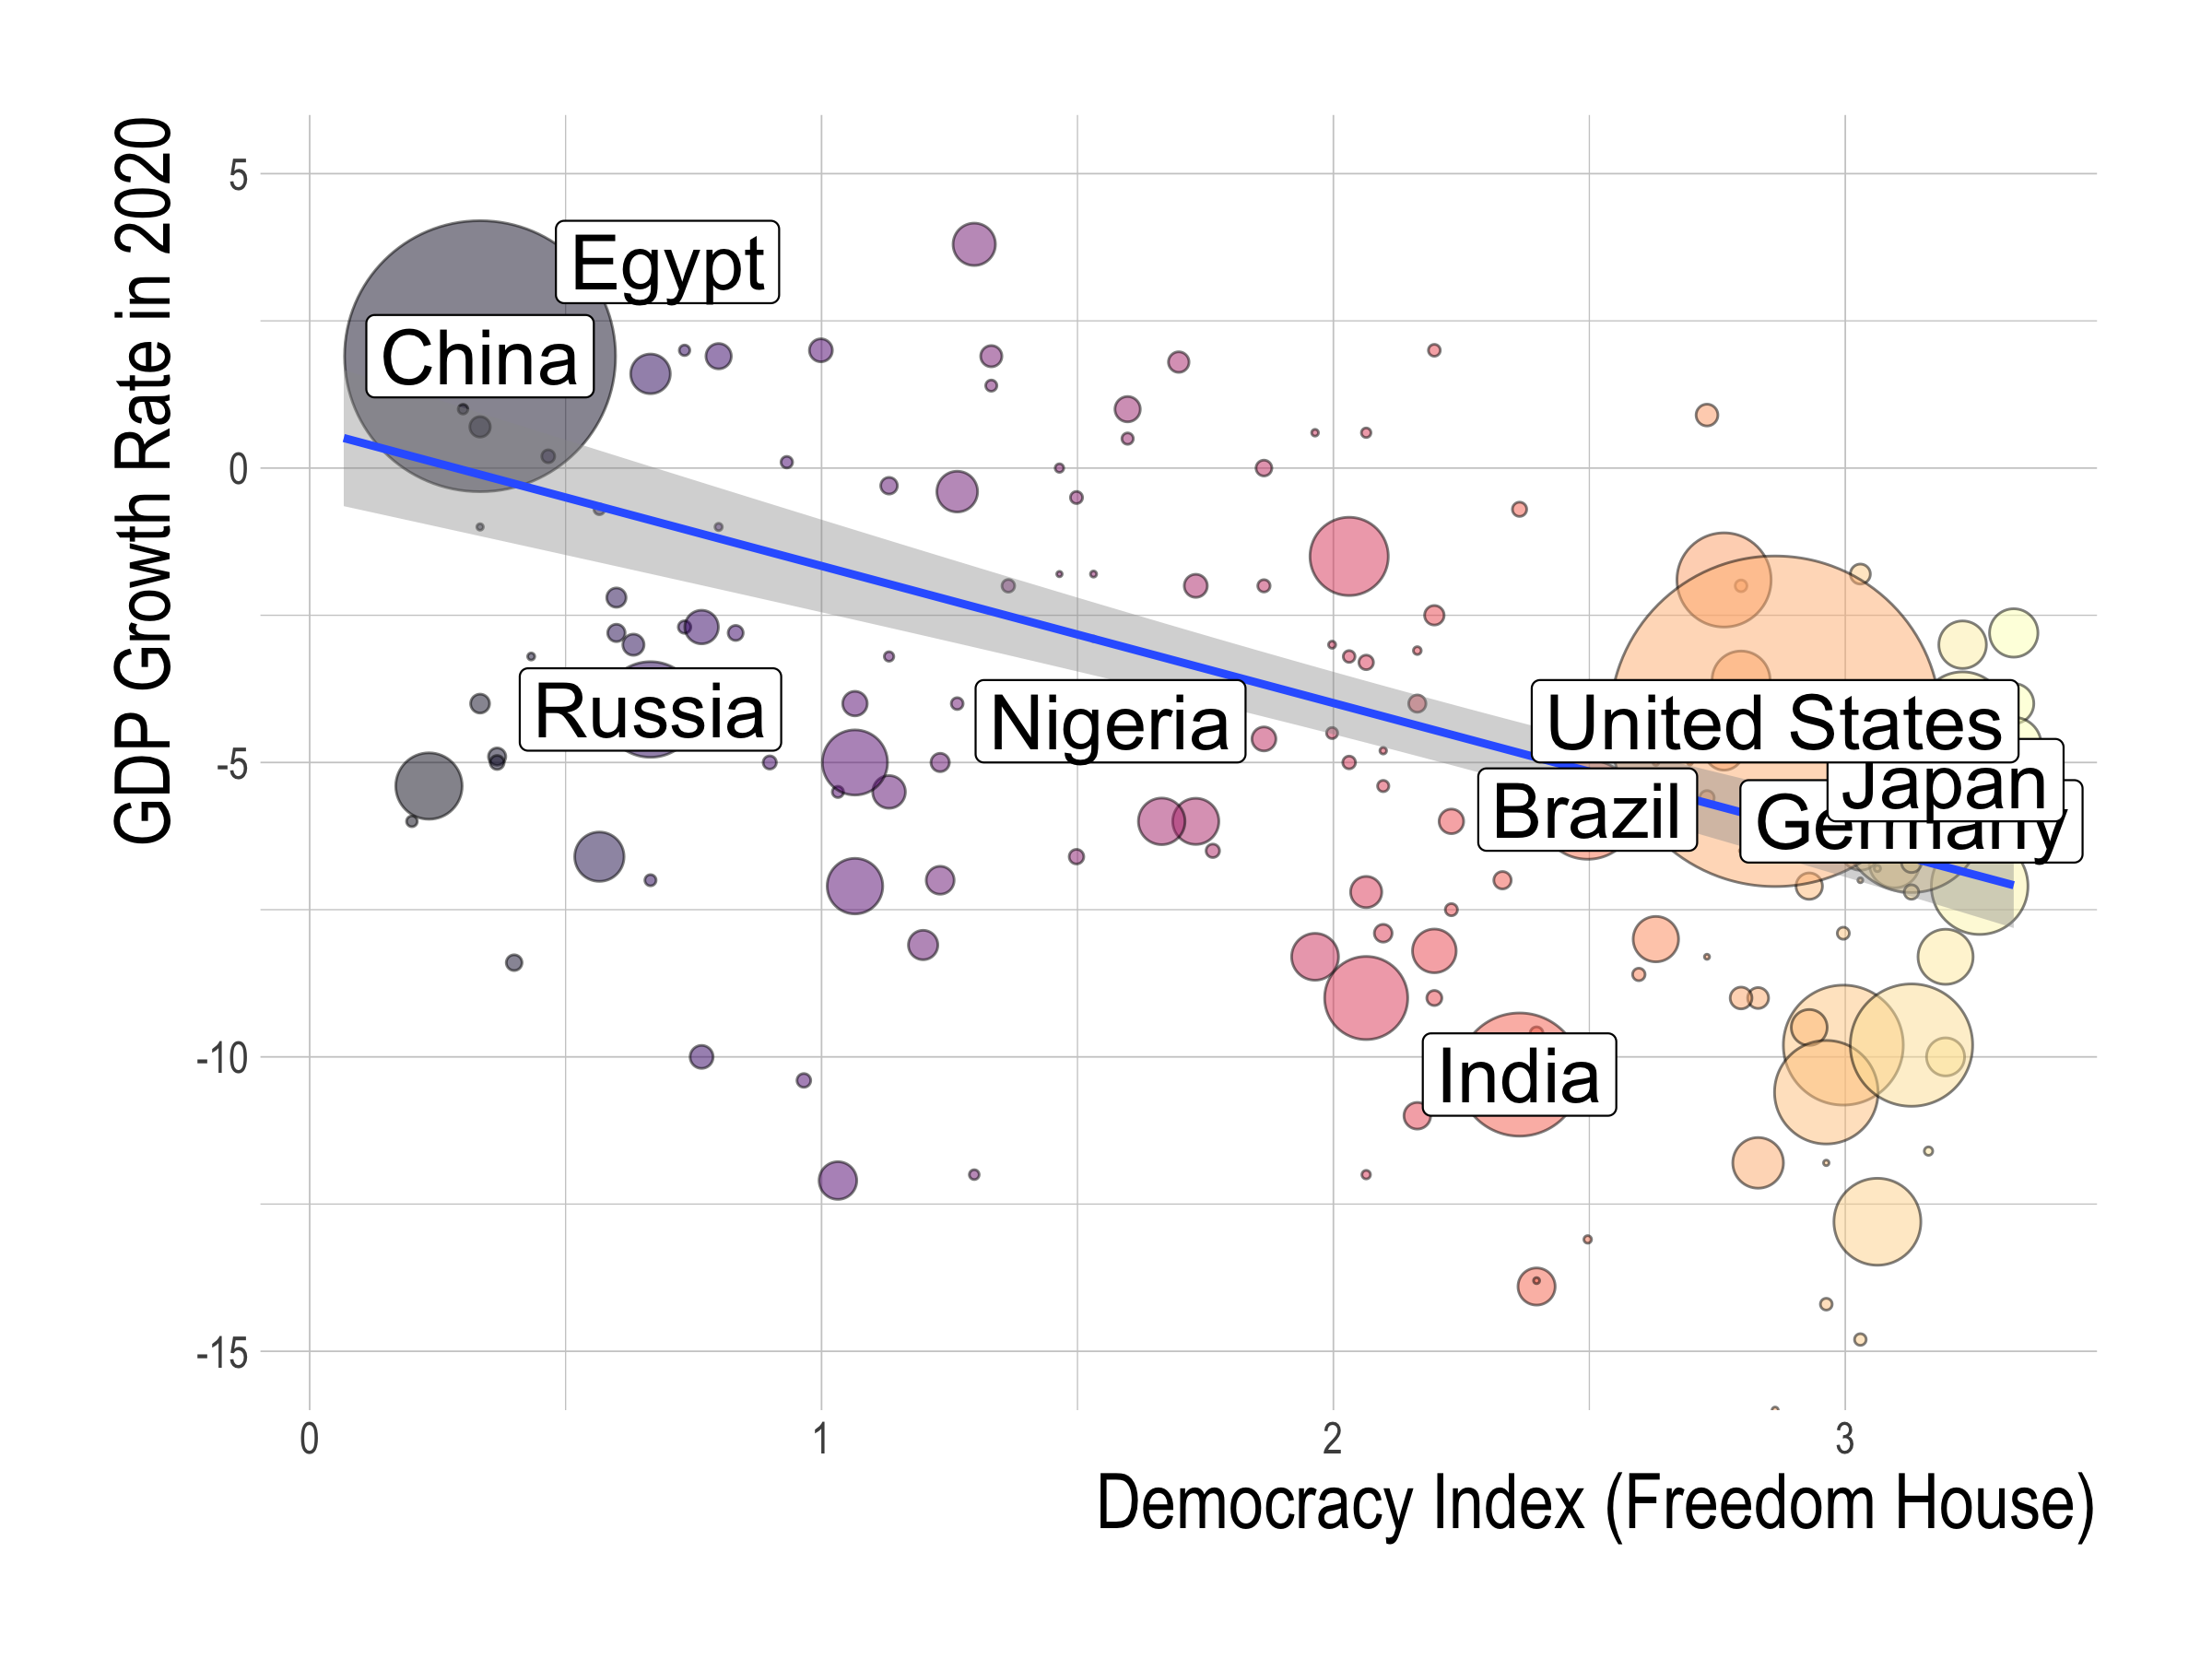
\includegraphics[width=4.4in]{plots/figure1a.png}}
  
  \subcaptionbox{Covid-19-related Deaths Per Million \label{fig:ols-deaths}}{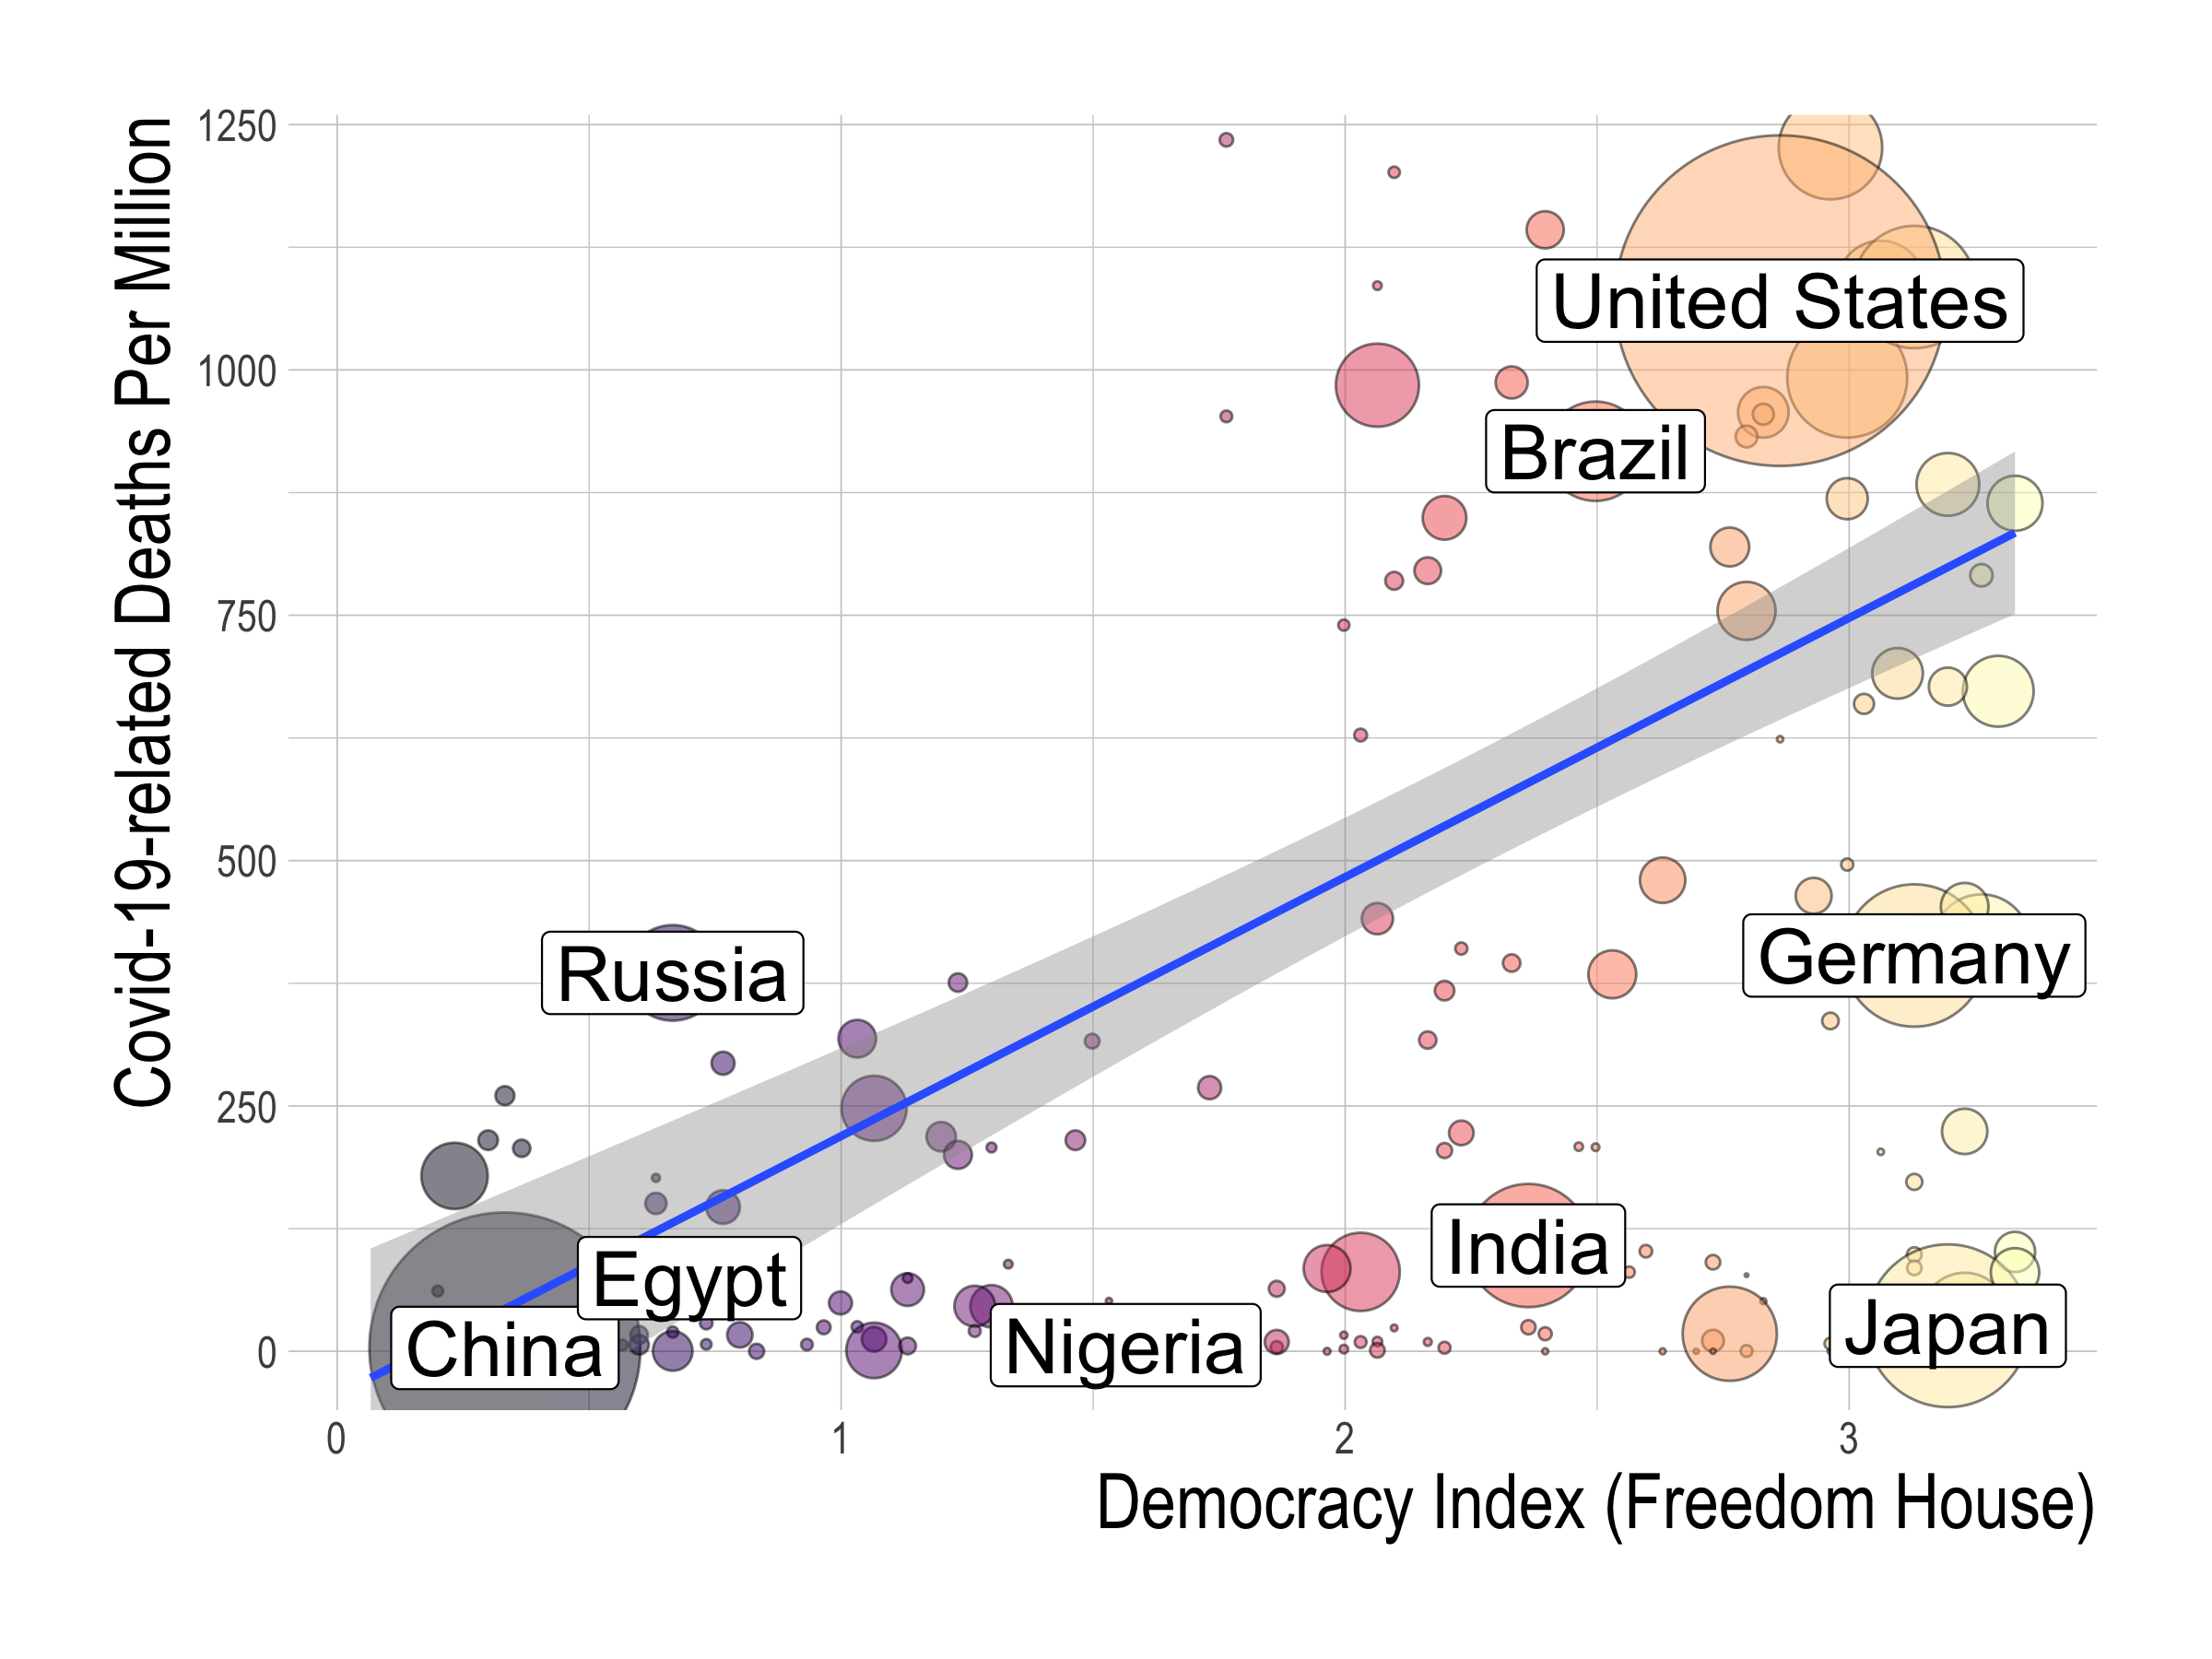
\includegraphics[width=4.4in]{plots/figure1b.png}}
  \caption*{\textit{Notes:} Figure (a) shows the relationship between democracy and GDP growth rates in 2020. Figure (b) shows the relationship between democracy and Covid-19-related deaths per million. The Democracy Index (Freedom House) is the sum of the political rights and civil liberties scales from \emph{Freedom in the World 2020} by Freedom House. It is normalized to have standard deviation one. The size of each observation point is proportional to the country's GDP. The colors depend on the level of the democracy index (warmer colors for democracy and darker colors for autocracies). The line is the fitted line from a univariate OLS regression of Covid-19 outcomes against the democracy index that weights observations by GDP. The shaded area corresponds to the 95\% confidence interval.}
\end{figure}

\newpage

% \newgeometry{left=0.5cm, right = 0.5cm, top=1.5cm}
\begin{figure}[htb]
\centering
\caption{Causal Effects of Democracy}\label{fig:first-stage}
\captionsetup{width=0.8\textwidth}
\begin{subfigure}[c]{.49\linewidth}

    \centering
    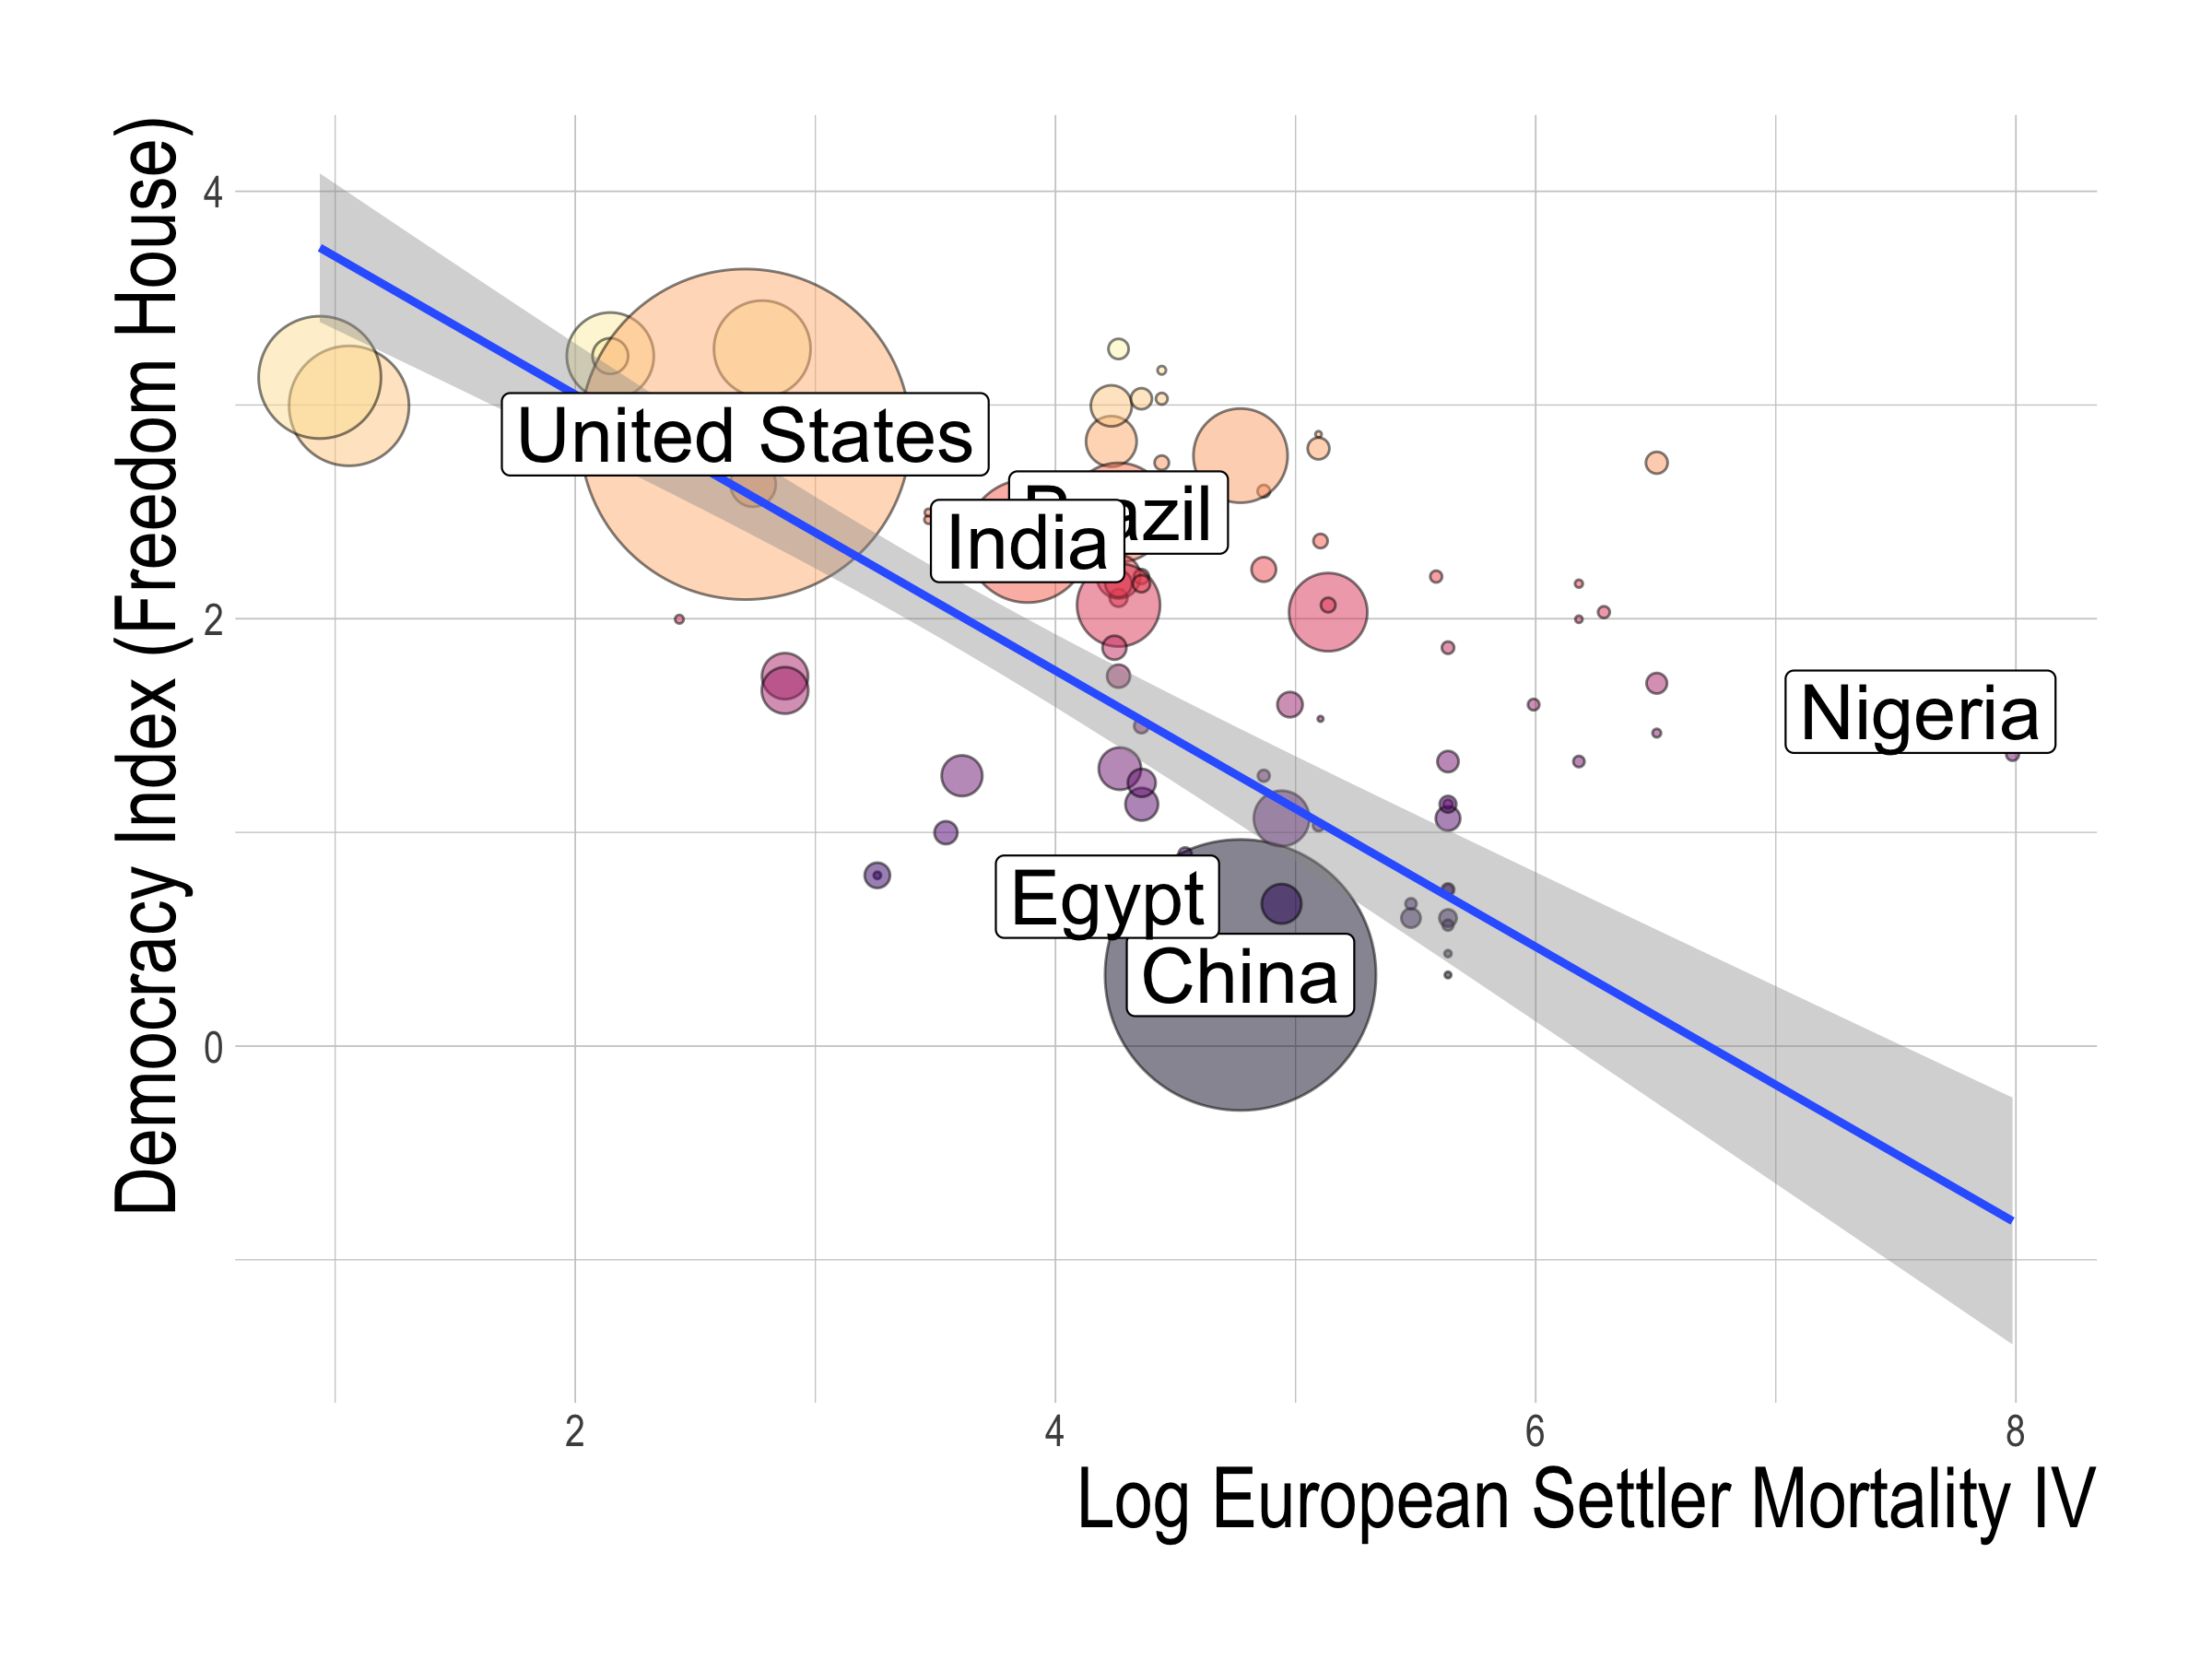
\includegraphics[width=.99\textwidth]{plots/figure2a.png}
    \caption{First-stage: Log European Settler Mortality IV}\label{fig:first-stage-european-settlers}
    
    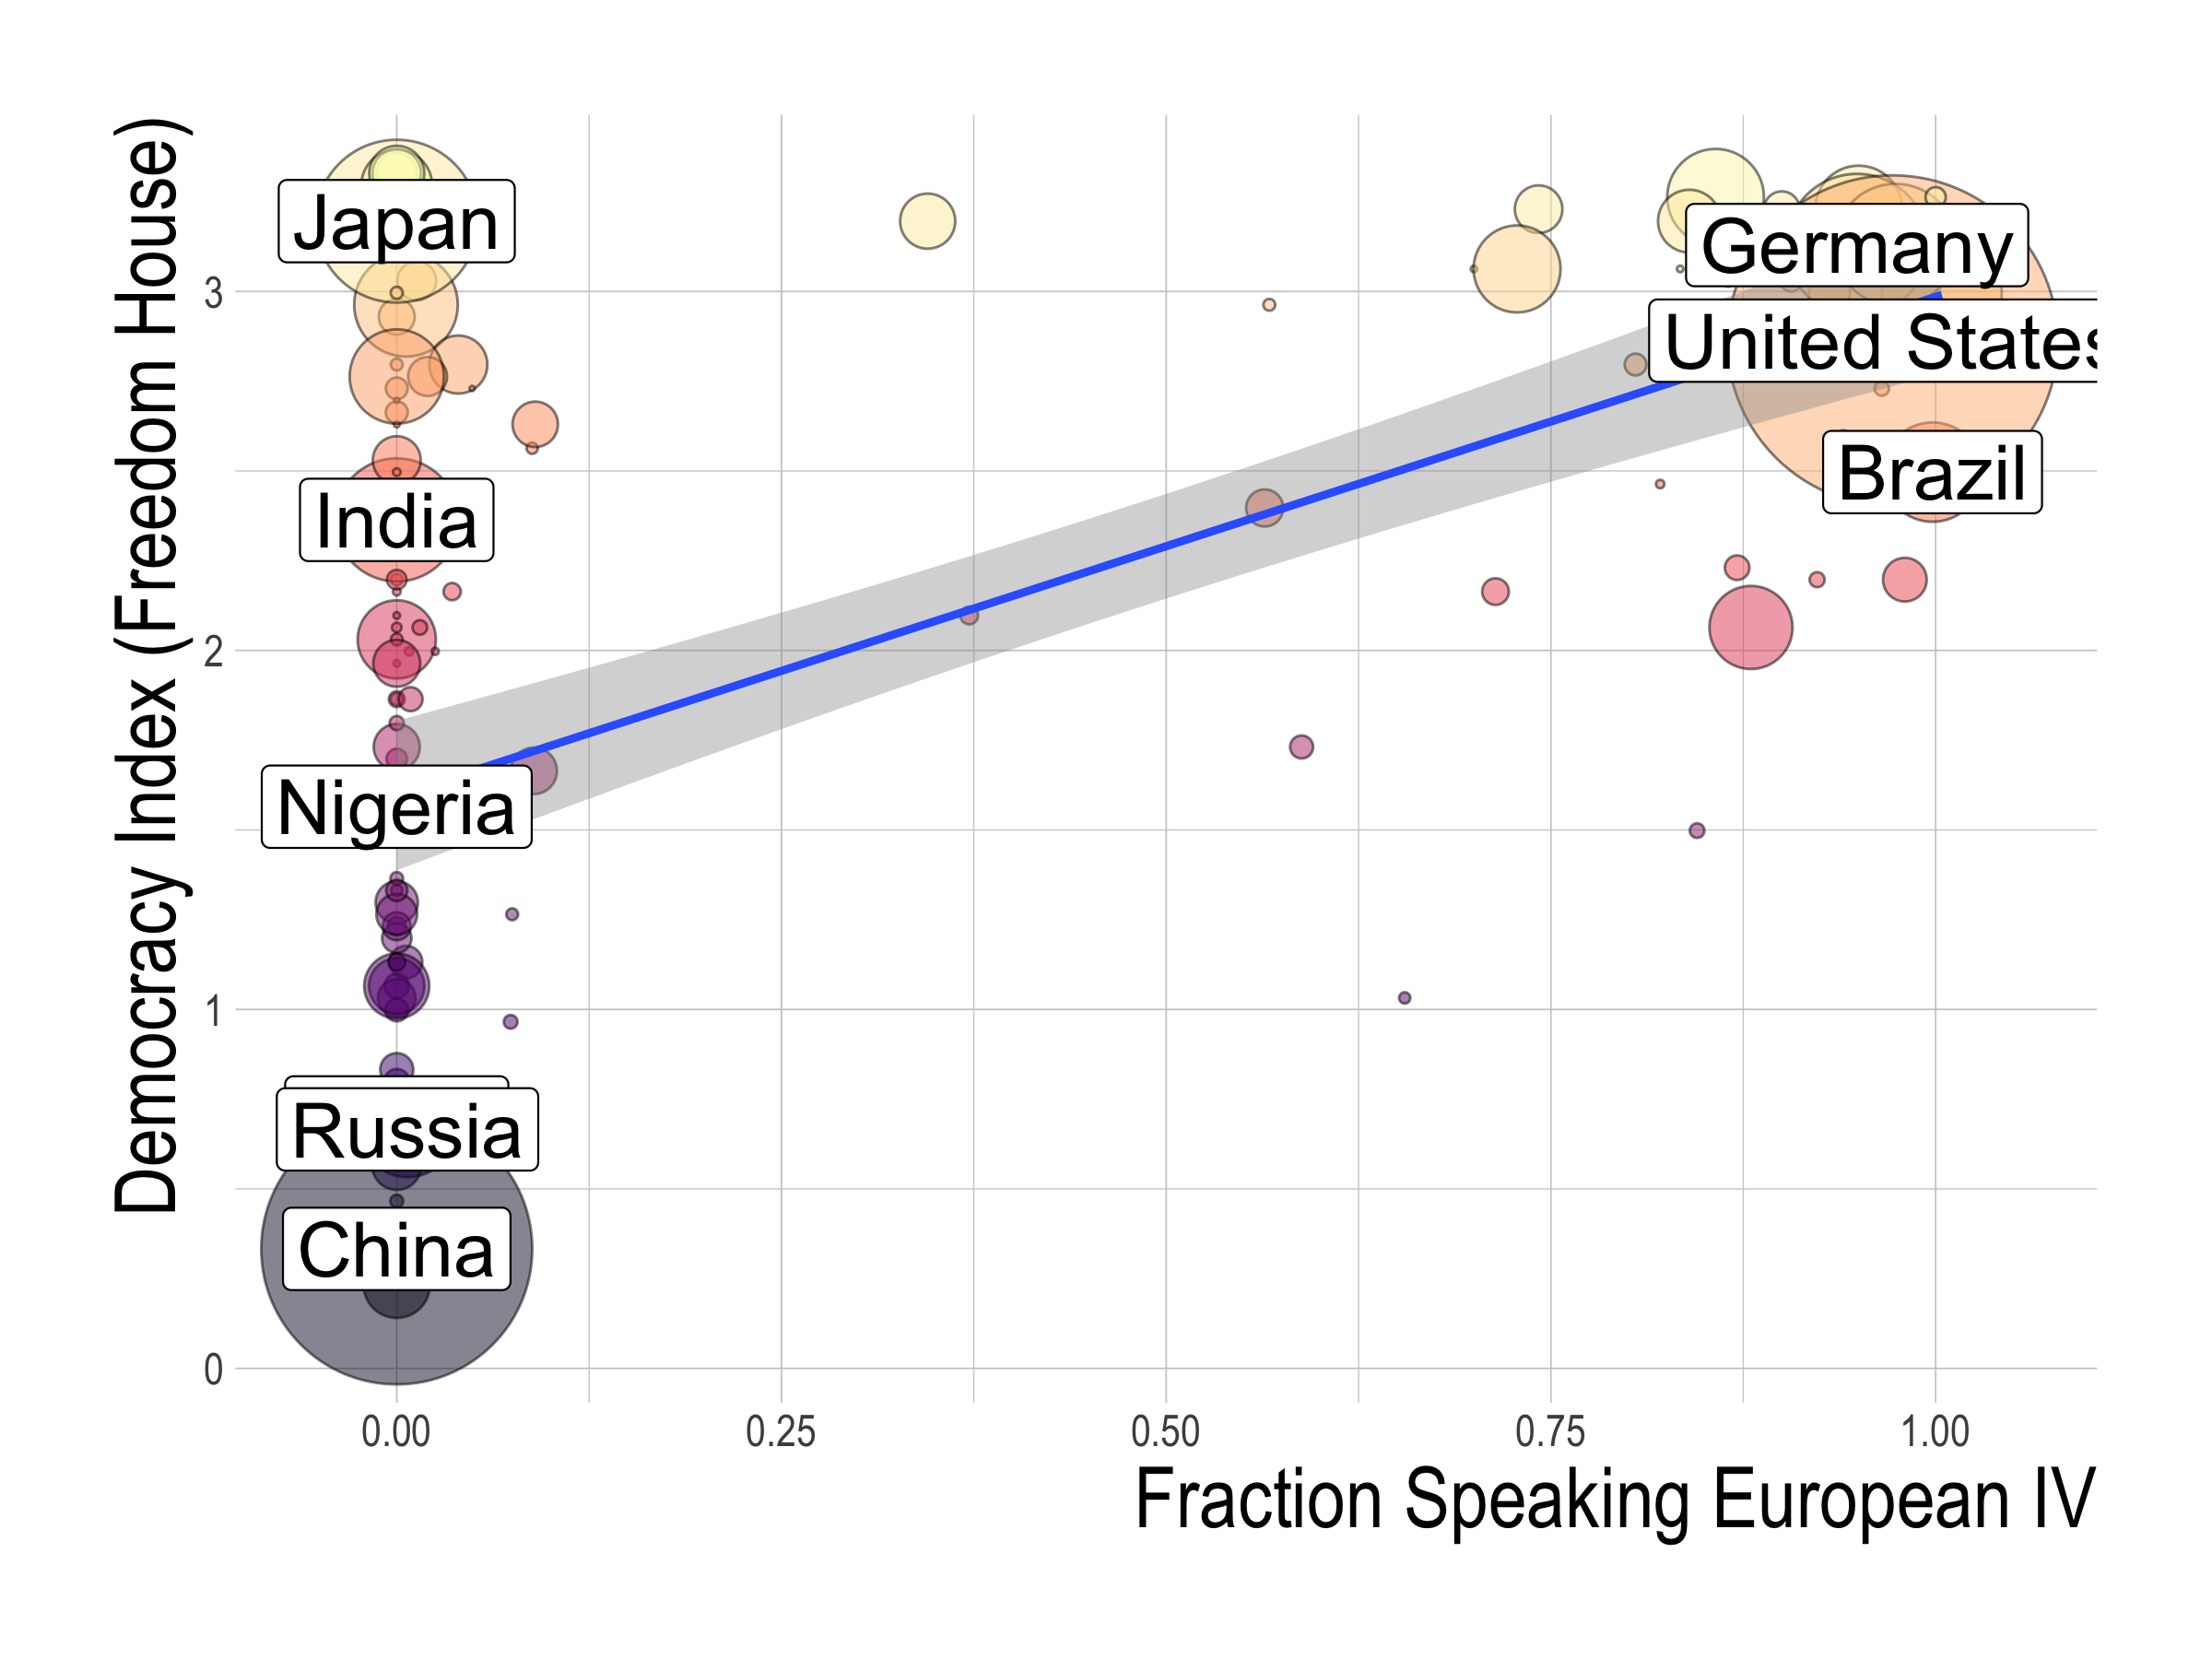
\includegraphics[width=.99\textwidth]{plots/figure2b.png}
    \caption{First-stage: Fraction Speaking European IV}\label{fig:first-stage-fraction-european}

\end{subfigure}
\begin{subfigure}[c]{.49\linewidth}
    \centering
    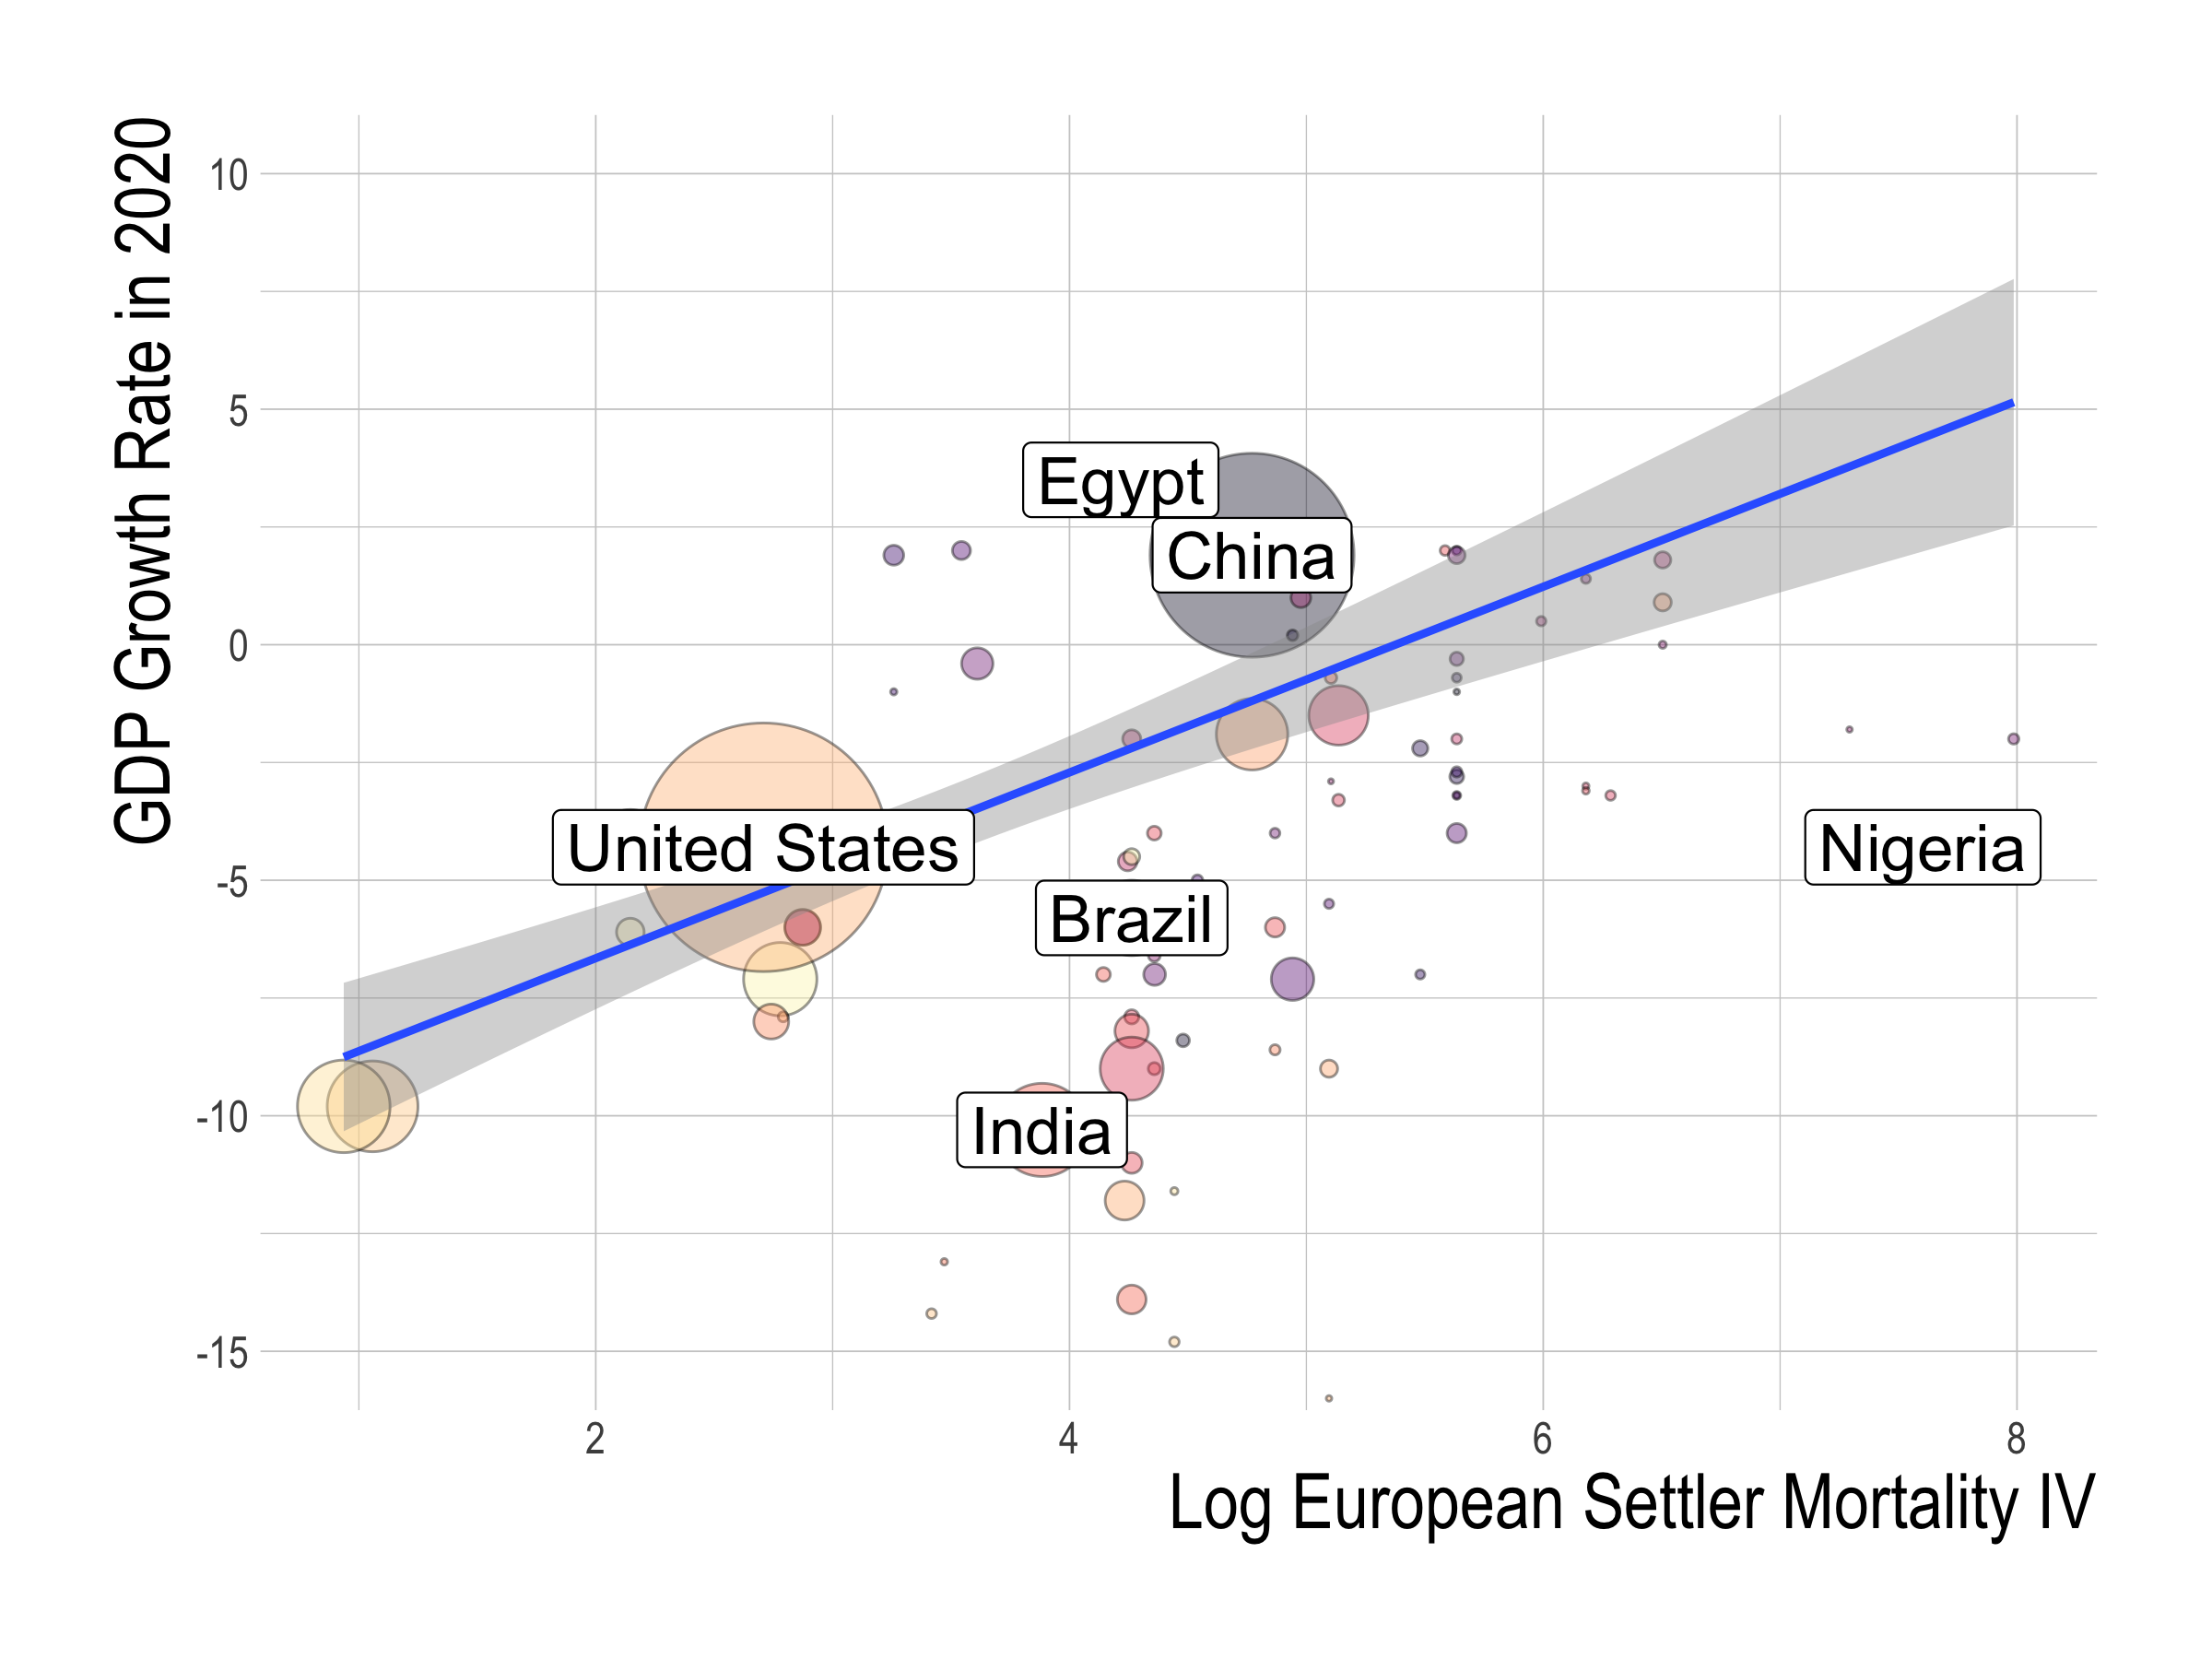
\includegraphics[width=.99\textwidth]{plots/figure2c.png}
    \caption{Reduced form: GDP Growth Rate in 2020}\label{fig:reduced-gdp-logem}
    
    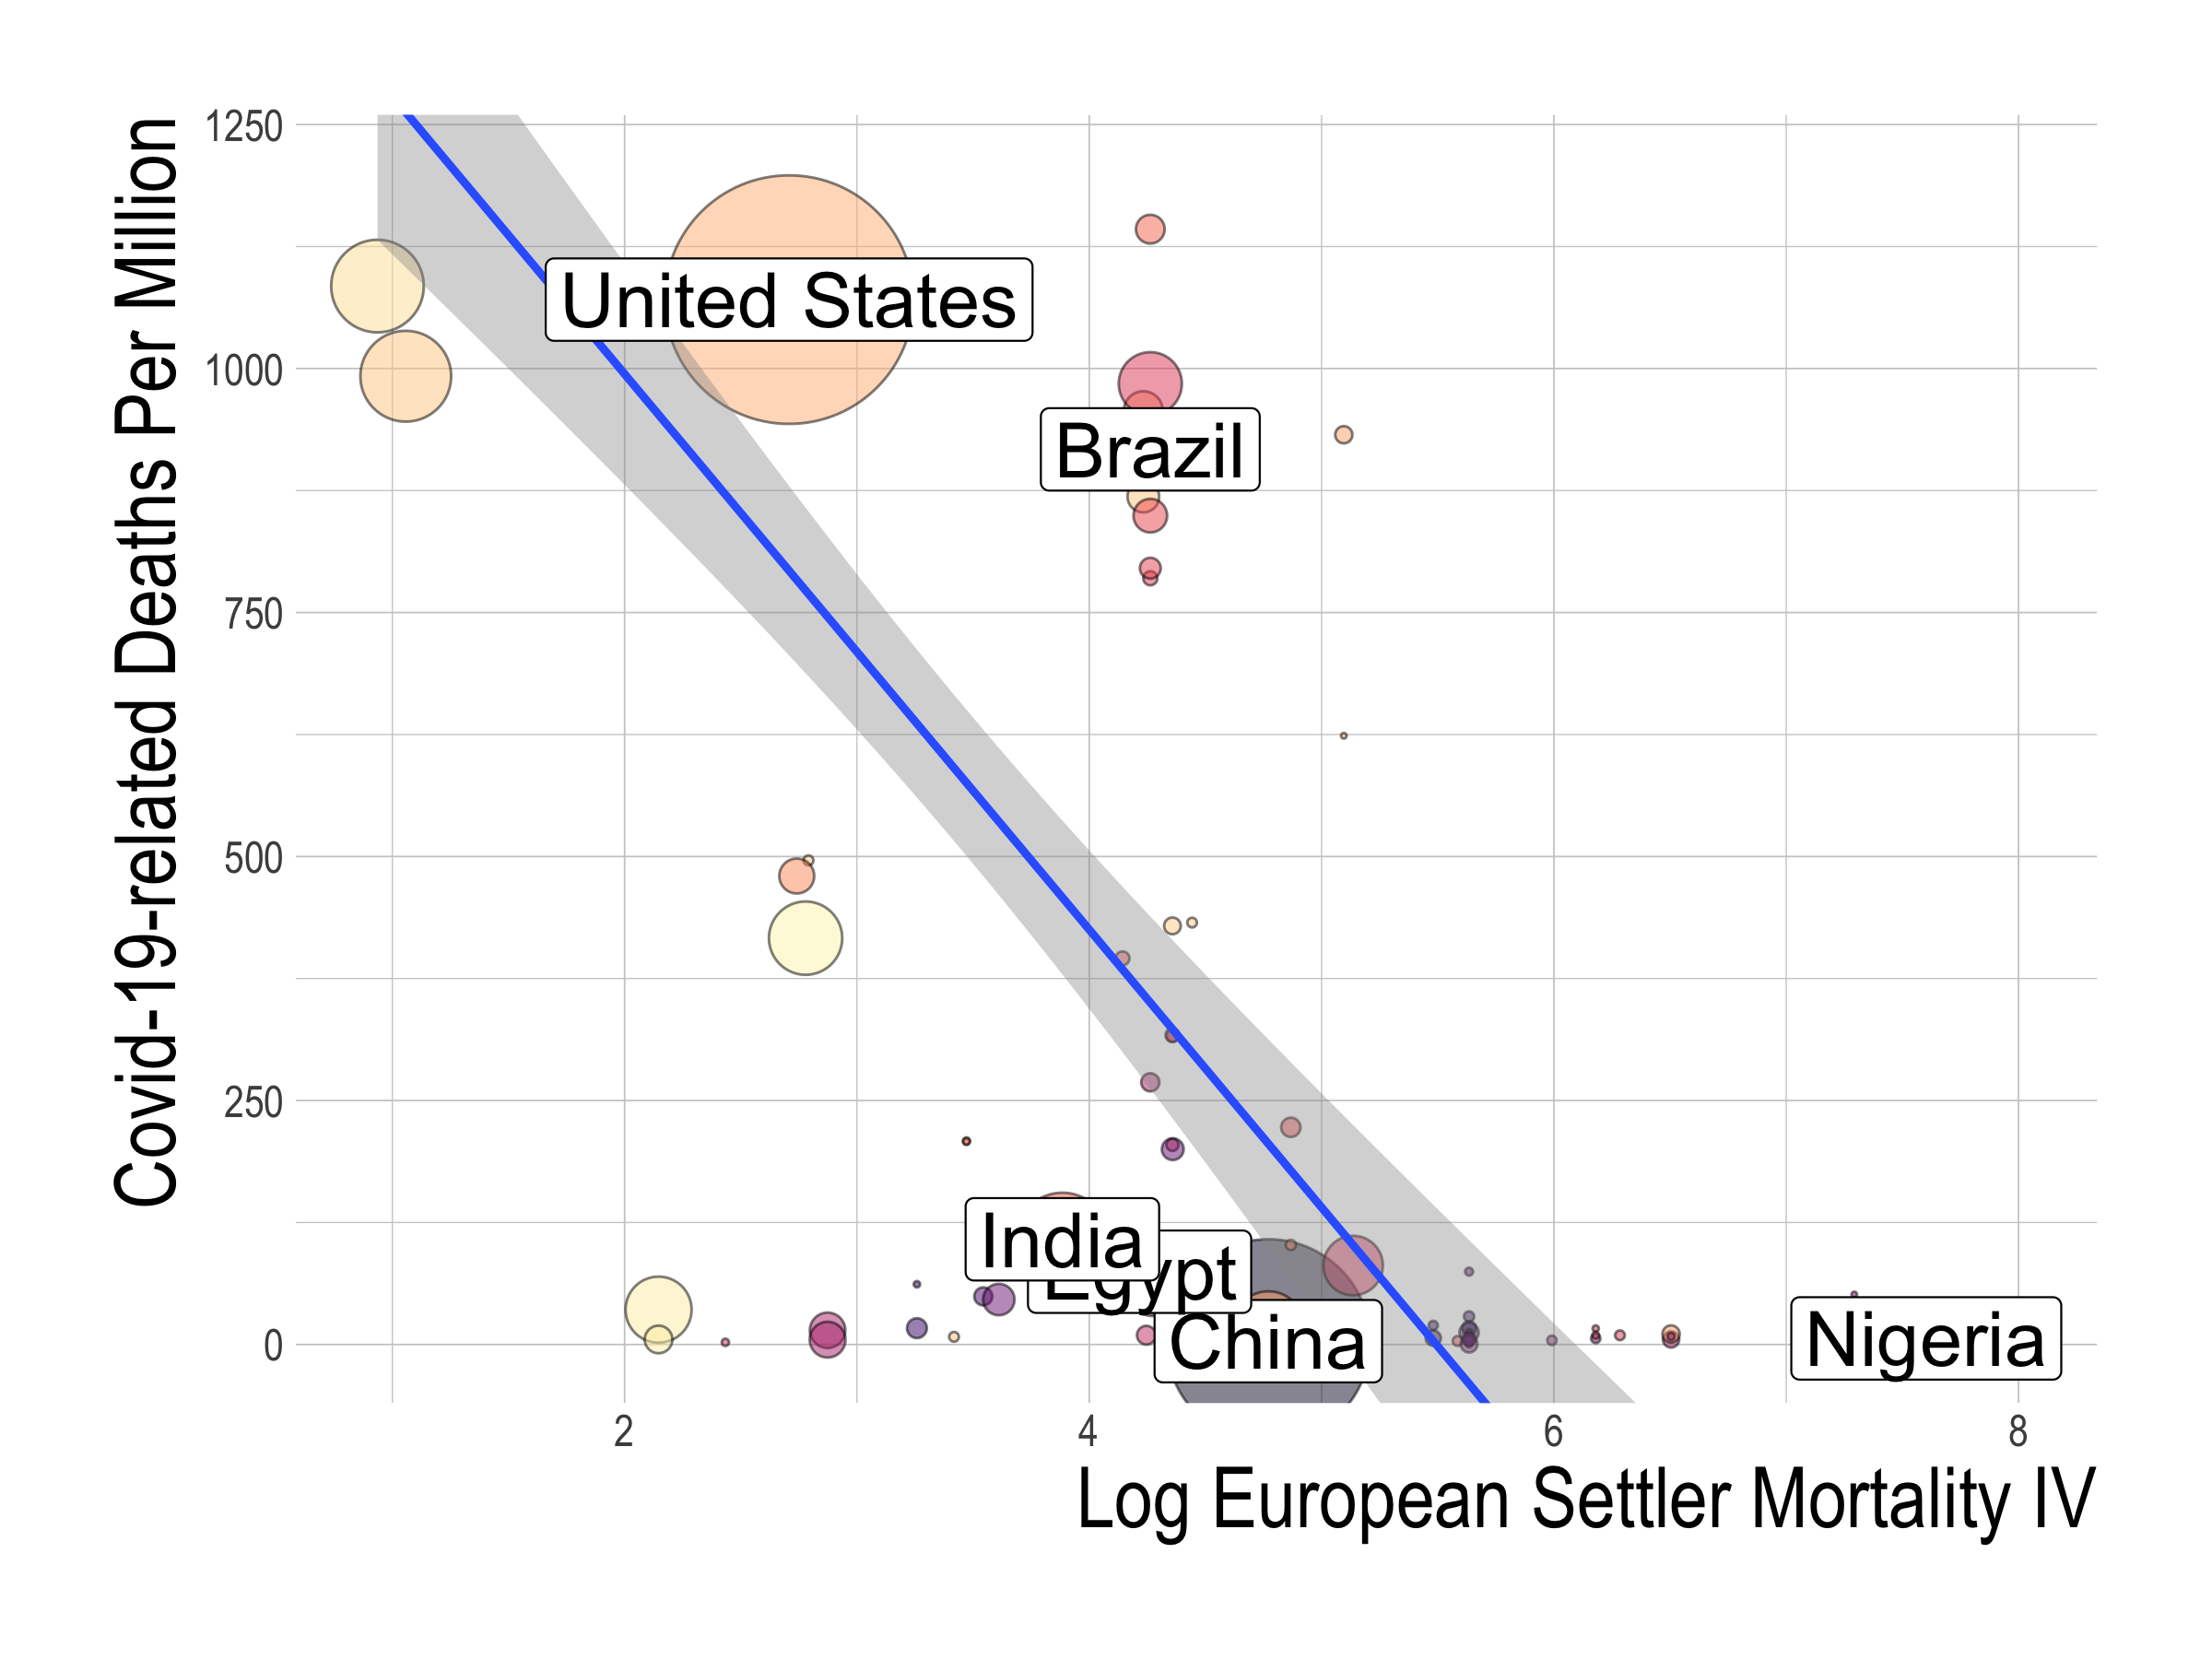
\includegraphics[width=.99\textwidth]{plots/figure2d.png}
    \caption{Reduced form: Covid-19-related Deaths Per Million}\label{fig:reduced-deaths-logem}
    
\end{subfigure}

\caption*{\textit{Notes:} Panels (a) and (b) show the first-stage relationship between democracy and two univariate IVs: the log European settler mortality IV and the fraction speaking European IV. Panels (c) and (d) show the reduced-form relationship between the log European settler mortality IV and Covid-19 outcomes: GDP growth rates in 2020 and Covid-19-related deaths per million. The Democracy Index (Freedom House) is the sum of the political rights and civil liberties scales from \emph{Freedom in the World 2020} by Freedom House. It is normalized to have standard deviation one. The size of each circle (country) is proportional to its GDP. The colors depend on the level of the democracy index. The line is the OLS regression fitted line without controls and weights countries by GDP. The shaded area corresponds to the 95\% confidence interval.}
\end{figure}


% \restoregeometry

% \newgeometry{left=1.75cm, top=1.5cm}

\begin{table}[!htbp]  \centering
  \caption{2SLS Regression Estimates of Democracy's Effects}
  \label{tab:2sls} 
  \footnotesize
  \begin{threeparttable}
\begin{tabular}{@{\extracolsep{0pt}}lcccccccccc} 
\\[-1.8ex]\hline 
\hline 
\\[-1.8ex] & (1) & (2) & (3) & (4) & (5) & (6) & (7) & (8) & (9) & (10)\\ 
\hline \\[-1.8ex] 
\multicolumn{11}{l}{\textbf{Panel A: Two-Stage Least Squares}} \\ 
  
 & \multicolumn{10}{c}{Dependent Variable is GDP Growth Rate in 2020} \\ 
\cline{2-11}  \\[-1.8ex]
Democracy Index     &        -3.1\sym{***}&        -2.6\sym{***}&        -2.7\sym{***}&        -2.1\sym{***}&        -3.5\sym{*}  &        -2.6\sym{***}&        -2.5\sym{***}&        -2.4\sym{***}&        -0.2         &        -2.1\sym{**} \\
                    &       (0.7)         &       (0.7)         &       (0.7)         &       (0.6)         &       (1.4)         &       (0.6)         &       (0.7)         &       (0.4)         &       (3.2)         &       (0.7)        \\ \\

 
& \multicolumn{10}{c}{Dependent Variable is Covid-19-related Deaths Per Million} \\ 
\cline{2-11}  \\[-1.8ex]
Democracy Index     &       440.5\sym{***}&       494.0\sym{***}&       416.9\sym{**} &       519.7\sym{***}&       550.4         &       483.9\sym{***}&       297.4\sym{***}&       389.1\sym{***}&      1035.2         &       486.4\sym{***}\\
                    &      (87.6)         &     (120.0)         &     (127.8)         &     (105.9)         &     (335.6)         &      (94.9)         &      (90.0)         &      (70.1)         &    (1051.3)         &     (137.9)         \\ \\
 % \hline \\[-1.8ex] 
 
% \multicolumn{11}{l}{\textbf{Panel B: First Stage for the Democracy Index}} \\ 

 %   & \multicolumn{10}{c}{Dependent Variable is Democracy Index} \\ 
% \cline{2-11}  \\[-1.8ex]
    IVs & \multicolumn{2}{c}{settler mortality} & \multicolumn{2}{c}{language \& trade} & \multicolumn{2}{c}{legal origins} &  \multicolumn{2}{c}{crops \& minerals} &  \multicolumn{2}{c}{pop. density} \\
    Number of IVs & 1 & 1 & 3 & 3 & 3 & 3 & 10 & 10 & 1 & 1 \\
\begin{comment}
Log European Settler Mortality&        -0.6\sym{**} &        -0.8\sym{**} &                     &                     &                     &                     &                     &                     &                     &                     \\
                    &       (0.2)         &       (0.3)         &                     &                     &                     &                     &                     &                     &                     &                     \\
Fraction Speaking English&                     &                     &         0.8\sym{*}  &         0.9\sym{*}  &                     &                     &                     &                     &                     &                     \\
                    &                     &                     &       (0.3)         &       (0.4)         &                     &                     &                     &                     &                     &                     \\
Fraction Speaking European&                     &                     &         1.0\sym{**} &         0.8\sym{***}&                     &                     &                     &                     &                     &                     \\
                    &                     &                     &       (0.3)         &       (0.2)         &                     &                     &                     &                     &                     &                     \\
Log Frankel-Romer Trade Share&                     &                     &         0.6\sym{**} &         0.2         &                     &                     &                     &                     &                     &                     \\
                    &                     &                     &       (0.2)         &       (0.2)         &                     &                     &                     &                     &                     &                     \\
British Legal Origin&                     &                     &                     &                     &        -0.5\sym{**} &         0.5         &                     &                     &                     &                     \\
                    &                     &                     &                     &                     &       (0.2)         &       (0.4)         &                     &                     &                     &                     \\
French Legal Origin &                     &                     &                     &                     &        -0.9\sym{***}&        -0.3         &                     &                     &                     &                     \\
                    &                     &                     &                     &                     &       (0.2)         &       (0.4)         &                     &                     &                     &                     \\
German Legal Origin &                     &                     &                     &                     &        -1.6         &        -1.0\sym{*}  &                     &                     &                     &                     \\
                    &                     &                     &                     &                     &       (0.8)         &       (0.4)         &                     &                     &                     &                     \\
Bananas             &                     &                     &                     &                     &                     &                     &        -0.1         &         0.1         &                     &                     \\
                    &                     &                     &                     &                     &                     &                     &       (0.4)         &       (0.4)         &                     &                     \\
Coffee              &                     &                     &                     &                     &                     &                     &        -0.3         &         0.6\sym{*}  &                     &                     \\
                    &                     &                     &                     &                     &                     &                     &       (0.2)         &       (0.3)         &                     &                     \\
Copper              &                     &                     &                     &                     &                     &                     &        -0.5         &         0.1         &                     &                     \\
                    &                     &                     &                     &                     &                     &                     &       (0.4)         &       (0.3)         &                     &                     \\
Maize               &                     &                     &                     &                     &                     &                     &         0.7\sym{*}  &         1.2\sym{*}  &                     &                     \\
                    &                     &                     &                     &                     &                     &                     &       (0.3)         &       (0.4)         &                     &                     \\
Millet              &                     &                     &                     &                     &                     &                     &        -0.5         &        -0.3         &                     &                     \\
                    &                     &                     &                     &                     &                     &                     &       (0.4)         &       (0.2)         &                     &                     \\
Rice                &                     &                     &                     &                     &                     &                     &        -0.9         &        -0.9\sym{*}  &                     &                     \\
                    &                     &                     &                     &                     &                     &                     &       (0.5)         &       (0.4)         &                     &                     \\
Rubber              &                     &                     &                     &                     &                     &                     &        -1.8\sym{***}&        -1.8\sym{***}&                     &                     \\
                    &                     &                     &                     &                     &                     &                     &       (0.5)         &       (0.3)         &                     &                     \\
Silver              &                     &                     &                     &                     &                     &                     &         1.0\sym{**} &         0.6         &                     &                     \\
                    &                     &                     &                     &                     &                     &                     &       (0.4)         &       (0.3)         &                     &                     \\
Sugarcane           &                     &                     &                     &                     &                     &                     &         1.2\sym{*}  &         0.7         &                     &                     \\
                    &                     &                     &                     &                     &                     &                     &       (0.5)         &       (0.4)         &                     &                     \\
Wheat               &                     &                     &                     &                     &                     &                     &        -0.3         &         0.9         &                     &                     \\
                    &                     &                     &                     &                     &                     &                     &       (0.4)         &       (0.5)         &                     &                     \\
Log Population Density in 1500s&                     &                     &                     &                     &                     &                     &                     &                     &       -0.08         &        -0.2\sym{***}\\
                    &                     &                     &                     &                     &                     &                     &                     &                     &       (0.1)         &      (0.07)         \\
                    
\end{comment}

% \(R^{2}\)           &         0.6         &         0.6         &         0.6         &         0.7         &         0.2         &         0.7         &         0.6         &         0.8         &        0.04         &         0.6         \\
F-statistics (First-Stage)                  &        10.1         &         4.3         &         4.7         &         8.8         &         6.8         &        12.6         &         8.8         &        10.3         &         0.7         &         5.3         \\

 \hline \\[-1.8ex] 

\multicolumn{11}{l}{\textbf{Panel B: Ordinary Least Squares}} \\ 
 & \multicolumn{10}{c}{Dependent Variable is GDP Growth Rate in 2020} \\ 
\cline{2-11}  \\[-1.8ex] 

Democracy Index &     -2.9\sym{***}&     -2.4\sym{***}&     -2.4\sym{***}&     -2.1\sym{***}&     -2.3\sym{***}&     -2.0\sym{***}&     -2.3\sym{***}&     -2.0\sym{***}&     -2.4\sym{***}&     -2.0\sym{***}\\
                &    (0.5)         &    (0.4)         &    (0.6)         &    (0.4)         &    (0.6)         &    (0.4)         &    (0.6)         &    (0.4)         &    (0.7)         &    (0.4)         \\
  \\

& \multicolumn{10}{c}{Dependent Variable is Covid-19-related Deaths Per Million} \\ 
\cline{2-11}  \\[-1.8ex]

Democracy Index &    347.0\sym{***}&    341.2\sym{***}&    264.0\sym{***}&    337.0\sym{***}&    264.0\sym{***}&    333.8\sym{***}&    264.6\sym{***}&    334.6\sym{***}&    277.9\sym{***}&    325.2\sym{***}\\
                &   (61.8)         &   (56.3)         &   (65.7)         &   (67.5)         &   (65.3)         &   (66.6)         &   (65.6)         &   (67.2)         &   (67.6)         &   (59.6)         \\

  \hline \\[-1.8ex] 
Controls & \xmark & \cmark & \xmark & \cmark & \xmark & \cmark & \xmark & \cmark & \xmark & \cmark\\ 
N &          85         &          85         &         140         &         140         &         168         &         168         &         149         &         149         &         155         &         155         \\
\hline 
\hline \\[-1.8ex] 
  & \multicolumn{10}{r}{$^{*}$p$<$0.1; $^{**}$p$<$0.05; $^{***}$p$<$0.01} \\ 
\end{tabular} 
\begin{tablenotes} 
\item {\footnotesize {\textit{Notes:} This table reports the 2SLS regression estimates of democracy's effect on Covid-19 outcomes, using five different IV strategies. The Democracy Index (Freedom House) is the sum of the political rights and civil liberties scales from \emph{Freedom in the World 2020} by Freedom House. It is normalized to have standard deviation one. Panel A reports the 2SLS estimates of the effect of democracy on GDP growth rates in 2020 and Covid-19-related deaths per million. The corresponding first-stage coefficients are in Appendix Table \ref{tab:first-stage}. Panel B reports the coefficients from OLS regressions of GDP growth rates in 2020 and Covid-19-related deaths per million against the democracy index. Columns 1, 3, 5, 7, and 9 have no controls, while columns 2, 4, 6, 8, and 10 have the following controls: absolute latitude, mean temperature, mean precipitation, population density, median age, and diabetes prevalence. %For all regressions, we weight observations by GDP. 
Robust standard errors are in parentheses. }}
\end{tablenotes}
\end{threeparttable}
\end{table} 

% This table reports the 2SLS regression estimates of democracy's effects and the results of its corresponding first-stage and OLS regressions. 

\begin{comment}
\begin{table}[!htbp] 
  \caption{2SLS Regression Estimates of Democracy's Effects}
  \label{tab:2sls} 
  \footnotesize
  \begin{threeparttable}
\begin{tabular}{@{\extracolsep{0pt}}lcccccccccc} 
\\[-1.8ex]\hline 
\hline 
\\[-1.8ex] & (1) & (2) & (3) & (4) & (5) & (6) & (7) & (8) & (9) & (10)\\ 
\hline \\[-1.8ex] 
\multicolumn{11}{l}{\textbf{Panel A: Two-Stage Least Squares}} \\ 
  
 & \multicolumn{10}{c}{Dependent Variable is GDP Growth Rate in 2020} \\ 
\cline{2-11}  \\[-1.8ex]
Democracy Index     &        -3.1\sym{***}&        -2.6\sym{***}&        -2.7\sym{***}&        -2.1\sym{***}&        -3.5\sym{*}  &        -2.6\sym{***}&        -2.5\sym{***}&        -2.4\sym{***}&        -0.2         &        -2.1\sym{**} \\
                    &       (0.7)         &       (0.7)         &       (0.7)         &       (0.6)         &       (1.4)         &       (0.6)         &       (0.7)         &       (0.4)         &       (3.2)         &       (0.7)         \\

 
& \multicolumn{10}{c}{Dependent Variable is Covid-19-related Deaths Per Million} \\ 
\cline{2-11}  \\[-1.8ex]
Democracy Index     &       440.5\sym{***}&       494.0\sym{***}&       416.9\sym{**} &       519.7\sym{***}&       550.4         &       483.9\sym{***}&       297.4\sym{***}&       389.1\sym{***}&      1035.2         &       486.4\sym{***}\\
                    &      (87.6)         &     (120.0)         &     (127.8)         &     (105.9)         &     (335.6)         &      (94.9)         &      (90.0)         &      (70.1)         &    (1051.3)         &     (137.9)         \\
 \hline \\[-1.8ex] 
 
\multicolumn{11}{l}{\textbf{Panel B: First Stage for the Democracy Index}} \\ 

   & \multicolumn{10}{c}{Dependent Variable is Democracy Index} \\ 
\cline{2-11}  \\[-1.8ex]
Log European Settler Mortality&        -0.6\sym{**} &        -0.8\sym{**} &                     &                     &                     &                     &                     &                     &                     &                     \\
                    &       (0.2)         &       (0.3)         &                     &                     &                     &                     &                     &                     &                     &                     \\
Fraction Speaking English&                     &                     &         0.8\sym{*}  &         0.9\sym{*}  &                     &                     &                     &                     &                     &                     \\
                    &                     &                     &       (0.3)         &       (0.4)         &                     &                     &                     &                     &                     &                     \\
Fraction Speaking European&                     &                     &         1.0\sym{**} &         0.8\sym{***}&                     &                     &                     &                     &                     &                     \\
                    &                     &                     &       (0.3)         &       (0.2)         &                     &                     &                     &                     &                     &                     \\
Log Frankel-Romer Trade Share&                     &                     &         0.6\sym{**} &         0.2         &                     &                     &                     &                     &                     &                     \\
                    &                     &                     &       (0.2)         &       (0.2)         &                     &                     &                     &                     &                     &                     \\
British Legal Origin&                     &                     &                     &                     &        -0.5\sym{**} &         0.5         &                     &                     &                     &                     \\
                    &                     &                     &                     &                     &       (0.2)         &       (0.4)         &                     &                     &                     &                     \\
French Legal Origin &                     &                     &                     &                     &        -0.9\sym{***}&        -0.3         &                     &                     &                     &                     \\
                    &                     &                     &                     &                     &       (0.2)         &       (0.4)         &                     &                     &                     &                     \\
German Legal Origin &                     &                     &                     &                     &        -1.6         &        -1.0\sym{*}  &                     &                     &                     &                     \\
                    &                     &                     &                     &                     &       (0.8)         &       (0.4)         &                     &                     &                     &                     \\
Bananas             &                     &                     &                     &                     &                     &                     &        -0.1         &         0.1         &                     &                     \\
                    &                     &                     &                     &                     &                     &                     &       (0.4)         &       (0.4)         &                     &                     \\
Coffee              &                     &                     &                     &                     &                     &                     &        -0.3         &         0.6\sym{*}  &                     &                     \\
                    &                     &                     &                     &                     &                     &                     &       (0.2)         &       (0.3)         &                     &                     \\
Copper              &                     &                     &                     &                     &                     &                     &        -0.5         &         0.1         &                     &                     \\
                    &                     &                     &                     &                     &                     &                     &       (0.4)         &       (0.3)         &                     &                     \\
Maize               &                     &                     &                     &                     &                     &                     &         0.7\sym{*}  &         1.2\sym{*}  &                     &                     \\
                    &                     &                     &                     &                     &                     &                     &       (0.3)         &       (0.4)         &                     &                     \\
Millet              &                     &                     &                     &                     &                     &                     &        -0.5         &        -0.3         &                     &                     \\
                    &                     &                     &                     &                     &                     &                     &       (0.4)         &       (0.2)         &                     &                     \\
Rice                &                     &                     &                     &                     &                     &                     &        -0.9         &        -0.9\sym{*}  &                     &                     \\
                    &                     &                     &                     &                     &                     &                     &       (0.5)         &       (0.4)         &                     &                     \\
Rubber              &                     &                     &                     &                     &                     &                     &        -1.8\sym{***}&        -1.8\sym{***}&                     &                     \\
                    &                     &                     &                     &                     &                     &                     &       (0.5)         &       (0.3)         &                     &                     \\
Silver              &                     &                     &                     &                     &                     &                     &         1.0\sym{**} &         0.6         &                     &                     \\
                    &                     &                     &                     &                     &                     &                     &       (0.4)         &       (0.3)         &                     &                     \\
Sugarcane           &                     &                     &                     &                     &                     &                     &         1.2\sym{*}  &         0.7         &                     &                     \\
                    &                     &                     &                     &                     &                     &                     &       (0.5)         &       (0.4)         &                     &                     \\
Wheat               &                     &                     &                     &                     &                     &                     &        -0.3         &         0.9         &                     &                     \\
                    &                     &                     &                     &                     &                     &                     &       (0.4)         &       (0.5)         &                     &                     \\
Log Population Density in 1500s&                     &                     &                     &                     &                     &                     &                     &                     &       -0.08         &        -0.2\sym{***}\\
                    &                     &                     &                     &                     &                     &                     &                     &                     &       (0.1)         &      (0.07)         \\
\(R^{2}\)           &         0.6         &         0.6         &         0.6         &         0.7         &         0.2         &         0.7         &         0.6         &         0.8         &        0.04         &         0.6         \\
F                   &        10.1         &         4.3         &         4.7         &         8.8         &         6.8         &        12.6         &         8.8         &        10.3         &         0.7         &         5.3         \\

 \hline \\[-1.8ex] 

\multicolumn{11}{l}{\textbf{Panel C: Ordinary Least Squares}} \\ 
 & \multicolumn{10}{c}{Dependent Variable is GDP Growth Rate in 2020} \\ 
\cline{2-11}  \\[-1.8ex] 

Democracy Index &     -2.9\sym{***}&     -2.4\sym{***}&     -2.4\sym{***}&     -2.1\sym{***}&     -2.3\sym{***}&     -2.0\sym{***}&     -2.3\sym{***}&     -2.0\sym{***}&     -2.4\sym{***}&     -2.0\sym{***}\\
                &    (0.5)         &    (0.4)         &    (0.6)         &    (0.4)         &    (0.6)         &    (0.4)         &    (0.6)         &    (0.4)         &    (0.7)         &    (0.4)         \\
  \\

& \multicolumn{10}{c}{Dependent Variable is Covid-19-related Deaths Per Million} \\ 
\cline{2-11}  \\[-1.8ex]

Democracy Index &    347.0\sym{***}&    341.2\sym{***}&    264.0\sym{***}&    337.0\sym{***}&    264.0\sym{***}&    333.8\sym{***}&    264.6\sym{***}&    334.6\sym{***}&    277.9\sym{***}&    325.2\sym{***}\\
                &   (61.8)         &   (56.3)         &   (65.7)         &   (67.5)         &   (65.3)         &   (66.6)         &   (65.6)         &   (67.2)         &   (67.6)         &   (59.6)         \\

  \hline \\[-1.8ex] 
Controls & \xmark & \cmark & \xmark & \cmark & \xmark & \cmark & \xmark & \cmark & \xmark & \cmark\\ 
N &          85         &          85         &         140         &         140         &         168         &         168         &         149         &         149         &         155         &         155         \\
\hline 
\hline \\[-1.8ex] 
  & \multicolumn{10}{r}{$^{*}$p$<$0.1; $^{**}$p$<$0.05; $^{***}$p$<$0.01} \\ 
\end{tabular} 
\begin{tablenotes} 
\item {\footnotesize {\textit{Notes:} This table reports the 2SLS regression estimates of democracy's effect on Covid-19 outcomes, using five different IV strategies. The Democracy Index (Freedom House) is the sum of the political rights and civil liberties scales from \emph{Freedom in the World 2020} by Freedom House. It is normalized to have standard deviation one. Panel A reports the 2SLS estimates of the effect of democracy on GDP growth rates in 2020 and Covid-19-related deaths per million. Panel B reports the corresponding first-stage regressions. Panel C reports the coefficients from OLS regressions of GDP growth rates in 2020 and Covid-19-related deaths per million against the democracy index. Columns 1, 3, 5, 7, and 9 have no controls, while columns 2, 4, 6, 8, and 10 have the following controls: absolute latitude, mean temperature, mean precipitation, population density, median age, and diabetes prevalence. %For all regressions, we weight observations by GDP. 
Robust standard errors are in parentheses. }}
\end{tablenotes}
\end{threeparttable}
\end{table} 

% This table reports the 2SLS regression estimates of democracy's effects and the results of its corresponding first-stage and OLS regressions. 

\end{comment}
\begin{table}[!htbp] \centering 
  \caption{2SLS Regressions on Potential Channels Behind Democracy's Effect} 
  \label{tab:channels} 
  \small
  \begin{threeparttable}
\begin{tabular}{@{\extracolsep{0pt}}lcccccccccc} 
\\[-1.8ex]\hline 
\hline \\[-1.8ex] 
 & (1) & (2) & (3) & (4) & (5) & (6) & (7) & (8) & (9) & (10)\\ 
\hline \\[-1.8ex] 
\textbf{ Panel A: Severity} & \multicolumn{10}{c}{ Dependent Variable is Containment Health Index at 10th Covid-19 Case} \\ 
\cline{2-11}  \\[-1.8ex]
Democracy Index     &        -0.4\sym{***}&        -0.4\sym{***}&        -0.4\sym{***}&        -0.4\sym{***}&        -0.5\sym{**} &        -0.5\sym{***}&        -0.4\sym{***}&        -0.5\sym{***}&        -0.9         &        -0.4\sym{***}\\
                    &      (0.08)         &      (0.09)         &      (0.07)         &      (0.06)         &       (0.2)         &      (0.07)         &      (0.06)         &      (0.04)         &       (0.5)         &      (0.07)         \\

 \textbf{ Panel B: Coverage} & \multicolumn{10}{c}{ Dependent Variable is Coverage of Containment Measures at 10th Covid-19 Case} \\ 
\cline{2-11}  \\[-1.8ex]
  Democracy Index     &        -9.5\sym{***}&        -8.6\sym{***}&        -9.5\sym{***}&       -11.5\sym{***}&       -12.7\sym{*}  &       -12.6\sym{***}&        -9.8\sym{***}&       -11.1\sym{***}&       -25.9         &       -12.0\sym{***}\\
                    &       (2.7)         &       (2.3)         &       (1.9)         &       (1.4)         &       (5.0)         &       (1.7)         &       (1.7)         &       (0.9)         &      (19.2)         &       (1.4)         \\

 \textbf { Panel C: Speed}  & \multicolumn{10}{c}{Dependent Variable is Days Between 10th Covid-19 Case and Any Containment Measure} \\ 
\cline{2-11}  \\[-1.8ex]
Democracy Index     &         0.7         &        -6.6\sym{**} &        0.03         &        -1.4         &       -10.8         &        -4.8\sym{*}  &        -0.7         &        -6.3\sym{***}&       -20.0         &        -6.2\sym{*}  \\
                    &       (4.1)         &       (2.4)         &       (3.3)         &       (2.2)         &       (8.1)         &       (2.4)         &       (2.9)         &       (1.7)         &      (24.8)         &       (3.1)         \\


 \hline \\[-1.8ex] 
    IVs & \multicolumn{2}{c}{settler mortality} & \multicolumn{2}{c}{language \& trade} & \multicolumn{2}{c}{legal origins} &  \multicolumn{2}{c}{crops \& minerals} &  \multicolumn{2}{c}{pop. density} \\
Controls & \xmark & \cmark & \xmark & \cmark & \xmark & \cmark & \xmark & \cmark & \xmark & \cmark\\ 
N   &          84         &          84         &         133         &         133         &         155         &         155         &         138         &         138         &         146         &         146         \\

\hline 
\hline \\[-1.8ex] 
  & \multicolumn{10}{r}{$^{*}$p$<$0.1; $^{**}$p$<$0.05; $^{***}$p$<$0.01} \\ 
\end{tabular} 
\begin{tablenotes} 
\item {\footnotesize {\textit{Notes:} This table reports the 2SLS regression estimates of democracy's effect on potential channels behind democracy's negative impact, using five different IV strategies. The Democracy Index (Freedom House) is the sum of the political rights and civil liberties scales from \textit{Freedom in the World 2020} by Freedom House. It is normalized to have standard deviation one. Panel A reports the 2SLS estimates of democracy's effect on the containment health index at the 10th confirmed case of Covid-19. The containment health index by the Oxford COVID-19 Government Response Tracker (OxCGRT) measures the strictness of containment policy. It is normalized to have standard deviation one. Panel B reports the 2SLS estimates of democracy's effect on the coverage of containment measures at the 10th confirmed case of Covid-19. The coverage of containment measures at the 10th confirmed Covid-19 case is the percentage across 13 domains where the government introduces any containment response. The domains are schools, workplaces, public events, gatherings, public transport, stay-at-home requirements, domestic travel, international travel, public information campaigns, testing, contact tracing, facial coverings, and vaccinations. Panel C reports the 2SLS estimates of democracy's effect on the number of days between the 10th confirmed case of Covid-19 and the introduction of any containment measure. We calculate the number of days between the 10th confirmed Covid-19 case and the introduction of any containment measure by subtracting the date when the 10th Covid-19 case is confirmed from the date when the containment health index becomes positive (all countries begin at zero). Columns 1, 3, 5, 7, and 9 have no controls, while columns 2, 4, 6, 8, and 10 have the following controls: absolute latitude, mean temperature, mean precipitation, population density, median age, and diabetes prevalence. For IVs, columns 1 and 2 use log European settler mortality, columns 3 and 4 use the fraction speaking English, the fraction speaking European, and the Frankel-Romer trade share, columns 5 and 6 use British legal origin, French legal origin, and German legal origin, columns 7 and 8 use the ability to grow crops and mine minerals (bananas, coffee, copper, maize, millet, rice, rubber, silver, sugarcane, and wheat), and columns 9 and 10 use log population density in the 1500s. For all regressions, we weight observations by GDP. Robust standard errors are in parentheses. }}
\end{tablenotes}
\end{threeparttable}
\end{table} 
\restoregeometry
% \addtolength{\hoffset}{0.75cm}
% \input{tables/2sls_gdp_freedom}
% 
\afterpage{% Insert after the current page
\clearpage
\thispagestyle{empty}
\KOMAoptions{paper=A3,paper=landscape, width=\textwidth}
\addtolength{\hoffset}{-12.0cm}
\addtolength{\voffset}{-6.0cm}
\recalctypearea


\begin{table}[] 
  \caption{2SLS regression on Covid-19-related deaths per million using the Freedom House index}
  \label{} 
  \small
  \begin{threeparttable}
\begin{tabular}{@{\extracolsep{0pt}}lcccccccccc} 
\\[-1.8ex]\hline 
\hline \\[-1.8ex] 
 & \multicolumn{10}{c}{\textit{Dependent variable:}} \\ 
\cline{2-11} 
\\[-1.8ex] & \multicolumn{10}{c}{Covid-19-related Deaths Per Million} \\ 
\\[-1.8ex] & (1) & (2) & (3) & (4) & (5) & (6) & (7) & (8) & (9) & (10)\\ 
\hline \\[-1.8ex] 
  & \multicolumn{10}{c}{Panel A: Two-Stage Least Squares} \\
Freedom House index & 645.1$^{***}$ & 472.1$^{***}$ & 370.1$^{***}$ & 453.2$^{***}$ & 340.6$^{**}$ & 506.8$^{***}$ & 356.3$^{***}$ & 173.1 & 484.0$^{***}$ & 528.0$^{***}$ \\ 
  & (239.7) & (71.7) & (67.8) & (59.1) & (155.9) & (121.2) & (120.2) & (108.8) & (152.8) & (151.8) \\ 
\hline \\[-1.8ex] 
   & \multicolumn{10}{c}{Panel B: First Stage for Freedom House index} \\
  Log European settler mortality & $-$0.3 & $-$0.4$^{**}$ &  &  &  &  &  &  &  &  \\ 
  & (0.2) & (0.2) &  &  &  &  &  &  &  &  \\ 
  Fraction speaking English &  &  & 0.8$^{***}$ & 1.0$^{**}$ &  &  &  &  &  &  \\ 
  &  &  & (0.2) & (0.4) &  &  &  &  &  &  \\ 
  Fraction speaking European &  &  & 1.4$^{***}$ & 1.0$^{***}$ &  &  &  &  &  &  \\ 
  &  &  & (0.2) & (0.2) &  &  &  &  &  &  \\ 
  Frankel-Romer trade share &  &  & 0.5$^{***}$ & 0.3$^{***}$ &  &  &  &  &  &  \\ 
  &  &  & (0.1) & (0.1) &  &  &  &  &  &  \\ 
  Legal origin: UK &  &  &  &  & 0.5 & 1.6$^{***}$ &  &  &  &  \\ 
  &  &  &  &  & (0.3) & (0.3) &  &  &  &  \\ 
  Legal origin: France &  &  &  &  & 0.6$^{***}$ & 1.4$^{***}$ &  &  &  &  \\ 
  &  &  &  &  & (0.2) & (0.2) &  &  &  &  \\ 
  Legal origin: Germany &  &  &  &  & $-$0.1 & 0.4 &  &  &  &  \\ 
  &  &  &  &  & (0.5) & (0.6) &  &  &  &  \\ 
  Legal origin: Scandinavian &  &  &  &  & 2.3$^{***}$ & 1.8$^{***}$ &  &  &  &  \\ 
  &  &  &  &  & (0.02) & (0.4) &  &  &  &  \\ 
  Landlock &  &  &  &  &  &  & $-$0.8$^{**}$ & $-$0.3 &  &  \\ 
  &  &  &  &  &  &  & (0.3) & (0.2) &  &  \\ 
  Oil &  &  &  &  &  &  & $-$0.3 & $-$0.4 &  &  \\ 
  &  &  &  &  &  &  & (0.4) & (0.3) &  &  \\ 
  Bananas &  &  &  &  &  &  & $-$0.9$^{**}$ & $-$0.4$^{*}$ &  &  \\ 
  &  &  &  &  &  &  & (0.3) & (0.2) &  &  \\ 
  Coffee &  &  &  &  &  &  & 0.02 & $-$0.3 &  &  \\ 
  &  &  &  &  &  &  & (0.3) & (0.3) &  &  \\ 
  Copper &  &  &  &  &  &  & 0.4 & $-$0.2 &  &  \\ 
  &  &  &  &  &  &  & (0.7) & (0.2) &  &  \\ 
  Maize &  &  &  &  &  &  & $-$0.1 & $-$1.6$^{**}$ &  &  \\ 
  &  &  &  &  &  &  & (0.7) & (0.8) &  &  \\ 
  Millet &  &  &  &  &  &  & $-$0.3 & $-$0.2 &  &  \\ 
  &  &  &  &  &  &  & (0.4) & (0.2) &  &  \\ 
  Rice &  &  &  &  &  &  & 0.4 & 0.4$^{***}$ &  &  \\ 
  &  &  &  &  &  &  & (0.4) & (0.1) &  &  \\ 
  Silver &  &  &  &  &  &  & 0.2 & $-$0.1 &  &  \\ 
  &  &  &  &  &  &  & (0.7) & (0.2) &  &  \\ 
  Sugarcane &  &  &  &  &  &  & 0.6 & 1.1$^{***}$ &  &  \\ 
  &  &  &  &  &  &  & (0.8) & (0.3) &  &  \\ 
  Rubber &  &  &  &  &  &  & $-$0.8$^{*}$ & 0.3 &  &  \\ 
  &  &  &  &  &  &  & (0.4) & (0.2) &  &  \\ 
  Wheat &  &  &  &  &  &  & $-$0.4 & $-$0.3 &  &  \\ 
  &  &  &  &  &  &  & (0.3) & (0.2) &  &  \\ 
  Log population density in 1500 &  &  &  &  &  &  &  &  & $-$0.2$^{**}$ & $-$0.2$^{**}$ \\ 
  &  &  &  &  &  &  &  &  & (0.1) & (0.1) \\ 
  R$^{2}$ & 0.1 & 0.4 & 0.6 & 0.8 & 0.1 & 0.5 & 0.4 & 0.8 & 0.1 & 0.5 \\ 
F Statistic & 9.5$^{***}$ (df = 1; 82) & 8.6$^{***}$ (df = 7; 76) & 60.7$^{***}$ (df = 3; 125) & 46.2$^{***}$ (df = 9; 119) & 5.0$^{***}$ (df = 4; 154) & 16.9$^{***}$ (df = 10; 148) & 3.2$^{***}$ (df = 12; 58) & 12.2$^{***}$ (df = 18; 52) & 26.3$^{***}$ (df = 1; 151) & 22.8$^{***}$ (df = 7; 145) \\ 
 \hline \\[-1.8ex] 
  & \multicolumn{10}{c}{Panel C: Ordinary Least Squares} \\
 Freedom House index & 307.0$^{***}$ & 356.0$^{***}$ & 261.3$^{***}$ & 318.2$^{***}$ & 257.1$^{***}$ & 290.5$^{***}$ & 365.2$^{***}$ & 296.2$^{***}$ & 264.2$^{***}$ & 299.0$^{***}$ \\ 
  & (60.7) & (40.6) & (52.2) & (51.0) & (50.1) & (49.8) & (79.0) & (83.9) & (23.7) & (26.5) \\ 
  R$^{2}$ & 0.6 & 0.7 & 0.5 & 0.6 & 0.4 & 0.6 & 0.5 & 0.7 & 0.5 & 0.6 \\ 
F Statistic & 108.6$^{***}$ (df = 1; 82) & 28.1$^{***}$ (df = 7; 76) & 105.1$^{***}$ (df = 1; 127) & 24.9$^{***}$ (df = 7; 121) & 125.2$^{***}$ (df = 1; 157) & 29.2$^{***}$ (df = 7; 151) & 79.2$^{***}$ (df = 1; 69) & 24.8$^{***}$ (df = 7; 63) & 124.1$^{***}$ (df = 1; 151) & 30.4$^{***}$ (df = 7; 145) \\ 
  \hline \\[-1.8ex] 
Weighting & Pop & Pop & Pop & Pop & Pop & Pop & Pop & Pop & Pop & Pop \\ 
Controls & \xmark & \cmark & \xmark & \cmark & \xmark & \cmark & \xmark & \cmark & \xmark & \cmark\\ 
N & 84 & 84 & 129 & 129 & 159 & 159 & 71 & 71 & 153 & 153 \\ 
\hline 
\hline \\[-1.8ex] 
 & \multicolumn{10}{r}{$^{*}$p$<$0.1; $^{**}$p$<$0.05; $^{***}$p$<$0.01} \\ 
\end{tabular} 
\begin{tablenotes} 
\item {\footnotesize {\textit{Note:} The Freedom House index is the sum of the political rights and civil liberties scales from Freedom in the World 2020 and has been normalized by its standard deviation. Panel A reports the two-stage least squares estimates of the effect of democracy on Covid-19-related deaths per million, using five different instrumental variable strategies. Panel B reports the corresponding first stage regressions. Panel C reports the coefficients from an OLS regression of the dependent variable against the Freedom House index.  Columns (1), (3), (5) and (7) have no controls, while columns (2), (4), (6) and (8) have the following controls: absolute latitude, mean temperature, mean precipitation, population density, median age and diabetes prevalence. All regressions have been weighted by population.}}
\end{tablenotes}
\end{threeparttable}
\end{table} 


\clearpage
\KOMAoptions{paper=A4,pagesize}
\recalctypearea
}


% \restoregeometry

\newpage
\section*{References}
\bibliographystyle{aea}
{\footnotesize
\bibliography{main_references}}



\newpage
\appendix
\setcounter{table}{0}
\renewcommand{\thetable}{\thesubsection\arabic{table}}
\setcounter{figure}{0}
\renewcommand{\thefigure}{\thesubsection\arabic{figure}}
\renewcommand{\thesubsection}{\Alph{subsection}}

\setcounter{table}{0}
\subsection{Additional Tables}

\begin{table}[!htbp]
    \centering
    \caption{Data Sources and Description} 
    \label{tab:sources}
    \scriptsize
\begin{tabularx}{\linewidth}{p{0.07\linewidth} p{0.2\linewidth} p{0.27\linewidth} p{0.36\linewidth}} 
    \hline \\[-1.8ex]
    & \textbf{Variable}  &  \textbf{Data Source} & \textbf{Short Description}\\ 
    \hline \\[-1.8ex]
    
    Outcomes 
    & GDP Growth Rate in 2020 & \citet{internationalmonetaryfundWorldEconomicOutlook2020} & Annual percentage change in real GDP between 2019 and 2020.\\
    
    & Covid-19-related Deaths Per Million & \citet{CSSE} & Total number of deaths per million attributed to Covid-19 between 2020/01/22 (earliest available in dataset) and 2020/12/31. \\
    
    & Covid-19 Cases Per Million & \citet{CSSE} & Total confirmed cases of Covid-19 per million between 2020/01/22 (earliest available in dataset) and 2020/12/31. \\
    \hline \\[-1.8ex]
    
    Treatments 
    
    & Democracy Index (Freedom House) & \citet{freedomhouseFreedomWorld20202020} &  Index measuring the degree of democratic freedom by taking the sum of the political rights (0 to 40) and civil liberties (0 to 60) scales. Ranges from 0 (least free) to 100 (most free).  \\
    
     & Democracy Index (Center for Systemic Peace) & \citet{centerforsystemicpeacePolity5AnnualTime2018} &  Index measuring the level of democracy by subtracting the autocracy score (0 (least autocratic) to 10 (most autocratic)) from the democracy score (0 (least democratic) to 10 (most democratic)). Ranges from -10 (strongly autocratic) to +10 (strongly democratic).\\ 
    
     & Democracy Index (Economist Intelligence Unit) & \citet{DemocracyIndex2020} & Index measuring the state of democracy. Ranges from 0 (least democratic) to 100 (most democratic). \\

\hline \\[-1.8ex]

    Weightings \& Controls 
    
    & GDP (Current USD, Billions) & \citet{theworldbankgroupGDPCurrentUS2020} & Gross domestic product at purchasing power parity in current U.S. billion dollars. Dollar figures for GDP are converted from domestic currencies using single year official exchange rates. \\ 
    
        & Population (Millions) & \citet{unitednationsdepartmentofeconomicandsocialaffairspopulationdivisionWorldPopulationProspects2019} & Total population in 2020 in millions. \\

    & Absolute Latitude & \citet{GooglePublicData} & Absolute value of the latitude of the centroid of each country (i.e., a measure of distance from the equator).\\
    
    & Mean Temperature & \citet{theworldbankgroupClimateChangeKnowledge2020} & The average of average monthly temperature from 1991-2016 in degrees Celcius. \\
    
    & Mean Precipitation & \citet{theworldbankgroupClimateChangeKnowledge2020} & The average of average monthly precipitation from 1991-2016 in millimeters. \\
    
    & Population Density & \citet{unitednationsdepartmentofeconomicandsocialaffairspopulationdivisionWorldPopulationProspects2019} & The number of people divided by land area, measured in square kilometers. \\
    
    & Median Age & \citet{unitednationsdepartmentofeconomicandsocialaffairspopulationdivisionWorldPopulationProspects2019} & UN projections of the median age of the population in 2020. \\
    
    & Diabetes Prevalence & \citet{internationaldiabetesfederationIDFDiabetesAtlas2019} & Percentage of population with diabetes aged 20 to 79 in 2017. \\ \hline \\[-1.8ex]
    

    IVs & 
    Log European Settler Mortality & \citet{ColonialOriginsReplicationData}. & The log of annualized deaths per thousand mean strength of European settlers between the seventeenth and nineteenth century.\\ %Original data from \citet{curtinDeathMigrationEurope1989}.
    
    & Fraction Speaking English & \citet{hallWhyCountriesProduceReplicationData}. & The fraction of the population speaking English as a mother tongue in 1992.\\ %Original data from \citet{hunterEthnologueLanguagesWorld1992, gunnemarkCountriesPeoplesTheir1991}
    
    & Fraction Speaking European & \citet{hallWhyCountriesProduceReplicationData}. & The fraction of the population speaking English, French, German, Portuguese or Spanish as a mother tongue in 1992.\\ %Original data from  \citet{hunterEthnologueLanguagesWorld1992, gunnemarkCountriesPeoplesTheir1991} 
    
    & Log Frankel-Romer Trade Share & \citet{hallWhyCountriesProduceReplicationData} & The log of Frankel-Romer predicted share based on Frankel and Romer (1999).\\ 
    
    & British Legal Origin, French Legal Origin, German Legal Origin & \citet{portaLawFinanceReplicationData} & Dummy variables coded 1 if the country's legal origin is British, French, or German, respectively, and 0 otherwise. \\
    
    & Bananas, Coffee, Maize, Millet, Rice, Sugarcane, Rubber, Wheat & \citet{easterlyReplicationData, foodandagricultureassociationoftheunitednationsFAOGlobalStatistical2020} & Dummy variables coded 1 if the country produced any of the particular commodity in 1990, and 0 otherwise. \\
    
    & Copper, Silver & \citet{easterlyReplicationData, CopperStatistics, SilverStatistics} & Dummy variables coded 1 if the country mined any of the particular commodity in 1990, and 0 otherwise. \\
    
    & Log Population Density in 1500s & \citet{UnbundlingInstitutionsReplicationData}. & The log of the population density in the 1500s measured as the number of inhabitants per square kilometer.  \\ \hline \\[-1.8ex] % Original data from \citet{mcevedyAtlasWorldPopulation1978}.
    
    Policy Responses &
    
    Containment Health Index at 10th Covid-19 Case & \citet{OxCGRT} & The containment health index measures the strictness of government responses by taking the average of 13 sub-scores that considers the severity and geographic scope of measures in its domain. The sub-scores first records severity on an ordinal scale (for example, the school sub-index is on a 0 (no measure) to 4 (require closing) scale) and subtracts 0.5 if it is targeted. Then, the scale is normalized. The domains are schools, workplaces, public events, gatherings, public transport, stay-at-home requirements, domestic travel, international travel, public information campaigns, testing, contact tracing, facial coverings, and vaccinations. We use the index at the date when the 10th case of Covid-19 is confirmed. \\
    
    & Coverage of Containment Measures at 10th Covid-19 Case & \citet{OxCGRT} & The percentage of the 13 domains in which the data records any policy introduction at the date when the 10th case of Covid-19 is confirmed. \\
    
    & Days between 10th Covid-19 Case and Any Containment Measure & \citet{OxCGRT} & The number of days between the date when the 10th Covid-19 case is confirmed and the date when the containment health index becomes positive. 
    
\\ \hline

\end{tabularx}
\end{table}


\newgeometry{left=0cm, right = 0cm}

\begin{table}[!htbp] \centering
  \caption{First-Stage Regression Estimates of IVs' Effects on Democracy}
  \label{tab:first-stage} 
  \footnotesize
  \begin{threeparttable}
\begin{tabular}{@{\extracolsep{0pt}}lcccccccccc} 
\\[-1.8ex]\hline 
\hline 
\\[-1.8ex] & (1) & (2) & (3) & (4) & (5) & (6) & (7) & (8) & (9) & (10)\\ 
\hline \\[-1.8ex] 
   & \multicolumn{10}{c}{Dependent Variable is Democracy Index} \\ 
\cline{2-11}  \\[-1.8ex]

Log European Settler Mortality&        -0.6\sym{**} &        -0.8\sym{**} &                     &                     &                     &                     &                     &                     &                     &                     \\
                    &       (0.2)         &       (0.3)         &                     &                     &                     &                     &                     &                     &                     &                     \\
Fraction Speaking English&                     &                     &         0.8\sym{*}  &         0.9\sym{*}  &                     &                     &                     &                     &                     &                     \\
                    &                     &                     &       (0.3)         &       (0.4)         &                     &                     &                     &                     &                     &                     \\
Fraction Speaking European&                     &                     &         1.0\sym{**} &         0.8\sym{***}&                     &                     &                     &                     &                     &                     \\
                    &                     &                     &       (0.3)         &       (0.2)         &                     &                     &                     &                     &                     &                     \\
Log Frankel-Romer Trade Share&                     &                     &         0.6\sym{**} &         0.2         &                     &                     &                     &                     &                     &                     \\
                    &                     &                     &       (0.2)         &       (0.2)         &                     &                     &                     &                     &                     &                     \\
British Legal Origin&                     &                     &                     &                     &        -0.5\sym{**} &         0.5         &                     &                     &                     &                     \\
                    &                     &                     &                     &                     &       (0.2)         &       (0.4)         &                     &                     &                     &                     \\
French Legal Origin &                     &                     &                     &                     &        -0.9\sym{***}&        -0.3         &                     &                     &                     &                     \\
                    &                     &                     &                     &                     &       (0.2)         &       (0.4)         &                     &                     &                     &                     \\
German Legal Origin &                     &                     &                     &                     &        -1.6         &        -1.0\sym{*}  &                     &                     &                     &                     \\
                    &                     &                     &                     &                     &       (0.8)         &       (0.4)         &                     &                     &                     &                     \\
Bananas             &                     &                     &                     &                     &                     &                     &        -0.1         &         0.1         &                     &                     \\
                    &                     &                     &                     &                     &                     &                     &       (0.4)         &       (0.4)         &                     &                     \\
Coffee              &                     &                     &                     &                     &                     &                     &        -0.3         &         0.6\sym{*}  &                     &                     \\
                    &                     &                     &                     &                     &                     &                     &       (0.2)         &       (0.3)         &                     &                     \\
Copper              &                     &                     &                     &                     &                     &                     &        -0.5         &         0.1         &                     &                     \\
                    &                     &                     &                     &                     &                     &                     &       (0.4)         &       (0.3)         &                     &                     \\
Maize               &                     &                     &                     &                     &                     &                     &         0.7\sym{*}  &         1.2\sym{*}  &                     &                     \\
                    &                     &                     &                     &                     &                     &                     &       (0.3)         &       (0.4)         &                     &                     \\
Millet              &                     &                     &                     &                     &                     &                     &        -0.5         &        -0.3         &                     &                     \\
                    &                     &                     &                     &                     &                     &                     &       (0.4)         &       (0.2)         &                     &                     \\
Rice                &                     &                     &                     &                     &                     &                     &        -0.9         &        -0.9\sym{*}  &                     &                     \\
                    &                     &                     &                     &                     &                     &                     &       (0.5)         &       (0.4)         &                     &                     \\
Rubber              &                     &                     &                     &                     &                     &                     &        -1.8\sym{***}&        -1.8\sym{***}&                     &                     \\
                    &                     &                     &                     &                     &                     &                     &       (0.5)         &       (0.3)         &                     &                     \\
Silver              &                     &                     &                     &                     &                     &                     &         1.0\sym{**} &         0.6         &                     &                     \\
                    &                     &                     &                     &                     &                     &                     &       (0.4)         &       (0.3)         &                     &                     \\
Sugarcane           &                     &                     &                     &                     &                     &                     &         1.2\sym{*}  &         0.7         &                     &                     \\
                    &                     &                     &                     &                     &                     &                     &       (0.5)         &       (0.4)         &                     &                     \\
Wheat               &                     &                     &                     &                     &                     &                     &        -0.3         &         0.9         &                     &                     \\
                    &                     &                     &                     &                     &                     &                     &       (0.4)         &       (0.5)         &                     &                     \\
Log Population Density in 1500s&                     &                     &                     &                     &                     &                     &                     &                     &       -0.08         &        -0.2\sym{***}\\
                    &                     &                     &                     &                     &                     &                     &                     &                     &       (0.1)         &      (0.07)         \\
                    
% \(R^{2}\)           &         0.6         &         0.6         &         0.6         &         0.7         &         0.2         &         0.7         &         0.6         &         0.8         &        0.04         &         0.6         \\
F-statistics                   &        10.1         &         4.3         &         4.7         &         8.8         &         6.8         &        12.6         &         8.8         &        10.3         &         0.7         &         5.3         \\

 \hline \\[-1.8ex] 

Controls & \xmark & \cmark & \xmark & \cmark & \xmark & \cmark & \xmark & \cmark & \xmark & \cmark\\ 
N &          85         &          85         &         140         &         140         &         168         &         168         &         149         &         149         &         155         &         155         \\
\hline 
\hline \\[-1.8ex] 
  & \multicolumn{10}{r}{$^{*}$p$<$0.1; $^{**}$p$<$0.05; $^{***}$p$<$0.01} \\ 
\end{tabular} 
\begin{tablenotes} 
\item {\footnotesize {\textit{Notes:} This table reports the first-stage regression estimates of the effect of the five different sets of IVs on democracy. It corresponds to the 2SLS estimates in Table \ref{tab:2sls}. The Democracy Index (Freedom House) is the sum of the political rights and civil liberties scales from \emph{Freedom in the World 2020} by Freedom House. It is normalized to have standard deviation one. Columns 1, 3, 5, 7, and 9 have no controls, while columns 2, 4, 6, 8, and 10 have the following controls: absolute latitude, mean temperature, mean precipitation, population density, median age, and diabetes prevalence. %For all regressions, we weight observations by GDP. 
Robust standard errors are in parentheses. }}
\end{tablenotes}
\end{threeparttable}
\end{table} 


\restoregeometry

\newgeometry{left=0cm, right = 0cm}

\begin{table}[!htbp] \centering
  \caption{GDP and Covid-19 Deaths without Democracy's Effect}
  \label{tab:remove-democracy-effect} 
  \footnotesize
  \begin{threeparttable}
\begin{tabular}{l*{6}{c}}
\hline\hline
                    &\multicolumn{1}{c}{(1)}&\multicolumn{1}{c}{(2)}&\multicolumn{1}{c}{(3)}&\multicolumn{1}{c}{(4)}&\multicolumn{1}{c}{(5)}&\multicolumn{1}{c}{(6)}\\
                    &      Africa&        Asia&      Europe&N. America&     Oceania&S. America\\
 \hline \\[-1.8ex]
 Panel A: GDP Growth Rate in 2020 & & & & & \\
 \hspace{3mm} Observed Mean &        -4.3&        -4.8&        -6.1&        -8.9&        -7.1&        -7.1\\
\hspace{3mm} Democracy's Estimated Effect  &        -4.4&        -4.0&        -8.0&        -7.8&        -8.4&        -7.3\\
 \hspace{3mm} After Subtracting Democracy's Effect&         0.2&        -0.7&         1.9&        -1.1&         1.3&         0.2\\ \\[-1.8ex] \hline \\[-1.8ex]
 Panel B: Total Covid-19-related Deaths Per Million & & & & & \\
\hspace{3mm} Observed Mean &        50.7&       151.9&       663.5&       312.1&         5.5&       594.8\\
\hspace{3mm} Democracy's Estimated Effect  &       631.3&       572.6&      1140.9&      1107.7&      1192.8&      1032.6\\
\hspace{3mm} After Subtracting Democracy's Effect&      -580.6&      -420.6&      -477.4&      -795.6&     -1187.3&      -437.8\\

\hline
N        &          53&          44&          45&          20&           8&          12\\
\hline\hline
\end{tabular}
\begin{tablenotes} 
\item {\footnotesize {\textit{Notes:} This table reports each continent's mean GDP growth rates in 2020 and total Covid-19-related deaths per million before and after subtracting the estimated effect of democracy in Table \ref{tab:2sls}'s column 1.}}
\end{tablenotes}
\end{threeparttable}
\end{table} 

\begin{comment}
Mean GDP Growth Rate in 2020&        -4.3&        -4.8&        -6.1&        -8.9&        -7.1&        -7.1\\
 \hspace{3mm} After Subtracting Democracy's Effect&         0.2&        -0.7&         1.9&        -1.1&         1.3&         0.2\\
Mean Total Covid-19-related Deaths Per Million&        50.7&       151.9&       663.5&       312.1&         5.5&       594.8\\
\hspace{3mm} After Subtracting Democracy's Effect&      -580.6&      -420.6&      -477.4&      -795.6&     -1187.3&      -437.8\\
\end{comment}

\restoregeometry


\newgeometry{top=0cm, bottom = 0cm}

\begin{landscape}
\begin{table}[!htbp] \centering 
  \caption{2SLS Regression with Alternative Democracy Indices} 
  \label{tab:2sls-compare-indices} 
    \begin{threeparttable}
\begin{tabular}{@{\extracolsep{0pt}}lcccccccccc} 
\\[-1.8ex]\hline 
\hline \\[-1.8ex] 
\\[-1.8ex] & (1) & (2) & (3) & (4) & (5) & (6) & (7) & (8) & (9) & (10)\\ 
\hline \\[-1.8ex] 
 & \multicolumn{10}{c}{\textit{Dependent variable:}} \\ 
\cline{2-11} 
\\[-1.8ex] & \multicolumn{10}{c}{Panel A: GDP Growth Rates in 2020} \\  \\
Democracy Index (Freedom House)   &        -3.1\sym{***}&        -2.7\sym{***}&        -2.7\sym{***}&        -2.1\sym{***}&        -3.5\sym{*}  &        -2.6\sym{***}&        -2.5\sym{***}&        -2.4\sym{***}&        -0.2         &        -2.1\sym{**} \\
                    &       (0.7)         &       (0.7)         &       (0.7)         &       (0.6)         &       (1.4)         &       (0.6)         &       (0.7)         &       (0.4)         &       (3.2)         &       (0.7)         \\
Democracy Index (Center for Systemic Peace)    &        -3.7\sym{***}&        -2.8\sym{***}&        -3.4\sym{***}&        -2.7\sym{***}&        -4.3\sym{**} &        -3.4\sym{***}&        -2.8\sym{***}&        -2.6\sym{***}&        -0.2         &        -2.4\sym{**} \\
                    &       (1.0)         &       (0.7)         &       (0.7)         &       (0.6)         &       (1.6)         &       (0.8)         &       (0.6)         &       (0.4)         &       (3.5)         &       (0.7)         \\
Democracy Index (Economist Intelligence Unit) &  -3.1\sym{***}&        -2.8\sym{***}&        -2.7\sym{***}&        -2.0\sym{***}&        -3.0\sym{*}  &        -2.5\sym{***}&        -2.6\sym{***}&        -2.5\sym{***}&        -0.2         &        -2.1\sym{**} \\
                    &       (0.7)         &       (0.7)         &       (0.7)         &       (0.6)         &       (1.2)         &       (0.5)         &       (0.8)         &       (0.5)         &       (2.7)         &       (0.7)         \\

 \hline \\[-1.8ex] 
 
  & \multicolumn{10}{c}{\textit{Dependent variable:} } \\ 
\cline{2-11} 
\\[-1.8ex] & \multicolumn{10}{c}{Panel B: Covid-19-related Deaths Per Million} \\ \\
Democracy Index (Freedom House)     &       440.4\sym{***}&       493.1\sym{***}&       417.6\sym{**} &       519.4\sym{***}&       552.6         &       484.2\sym{***}&       297.4\sym{***}&       389.4\sym{***}&      1033.0         &       486.1\sym{***}\\
                    &      (87.5)         &     (119.8)         &     (128.0)         &     (105.8)         &     (337.4)         &      (95.1)         &      (90.2)         &      (70.2)         &    (1047.9)         &     (137.9)         \\
Democracy Index (Center for Systemic Peace)    &       539.9\sym{**} &       525.7\sym{***}&       494.5\sym{*}  &       644.3\sym{***}&       588.9         &       603.0\sym{***}&       312.6\sym{**} &       388.8\sym{***}&      1153.7         &       543.5\sym{**} \\
                    &     (169.3)         &     (144.2)         &     (203.4)         &     (178.6)         &     (390.4)         &     (159.0)         &     (108.5)         &      (92.2)         &    (1215.1)         &     (178.2)         \\

Democracy Index  (Economist Intelligence Unit)   &       442.0\sym{***}&       515.6\sym{***}&       415.5\sym{***}&       519.0\sym{***}&       492.2         &       460.0\sym{***}&       306.9\sym{***}&       415.7\sym{***}&       875.1         &       470.5\sym{***}\\
                    &      (90.4)         &     (132.6)         &     (121.8)         &     (107.0)         &     (257.4)         &      (95.5)         &      (86.3)         &      (71.1)         &     (689.6)         &     (134.4)         \\
 \hline \\[-1.8ex] 
   IVs & \multicolumn{2}{c}{settler mortality} & \multicolumn{2}{c}{language \& trade} & \multicolumn{2}{c}{legal origins} &  \multicolumn{2}{c}{crops \& minerals} &  \multicolumn{2}{c}{pop. density} \\
Controls & \xmark & \cmark & \xmark & \cmark & \xmark & \cmark & \xmark & \cmark & \xmark & \cmark\\ 
N  &          81         &          81         &         128         &         128         &         152         &         152         &         134         &         134         &         145         &         145         \\

\hline 
\hline \\[-1.8ex] 
 & \multicolumn{10}{r}{$^{*}$p$<$0.1; $^{**}$p$<$0.05; $^{***}$p$<$0.01} \\ 
\end{tabular} 
\begin{tablenotes}
\item {\footnotesize {\textit{Notes:} This table compares the results of 2SLS regressions on Covid-19 outcomes using democracy indices by Freedom House, the Center for Systemic Peace, and the Economist Intelligence Unit. We normalize all indices to have standard deviation one. Panel A shows the 2SLS estimates of democracy's effect on GDP growth rates in 2020. Panel B shows the 2SLS estimates of democracy's effect on Covid-19 related deaths per million. Columns 1, 3, 5, 7, and 9 have no controls, while columns 2, 4, 6, 8, and 10 have the following controls: absolute latitude, mean temperature, mean precipitation, population density, median age, and diabetes prevalence. For IVs, columns 1 and 2 use log European settler mortality, columns 3 and 4 use the fraction speaking English, the fraction speaking European, and the Frankel-Romer trade share, columns 5 and 6 use British legal origin, French legal origin, and German legal origin, columns 7 and 8 use the ability to grow crops and mine minerals (bananas, coffee, copper, maize, millet, silver, sugarcane, rice, rubber, and wheat), and columns 9 and 10 use log population density in the 1500s. For all regressions, we weight observations by GDP. The estimates in this table are slightly different from those in Table \ref{tab:2sls} because some observations with missing data for the other democracy indices are removed for comparability across indices. Robust standard errors are in parentheses.}}
\end{tablenotes}
\end{threeparttable}
\end{table}
\end{landscape}


\restoregeometry

\newgeometry{top=0cm, bottom = 0cm, right = 1cm, left = 1.5cm}
\begin{landscape}
\begin{table}[!htbp] \centering 
  \caption{2SLS Regression with Alternative Weightings} 
  \label{tab:2sls-compare-weighting} 
  \begin{threeparttable}
\begin{tabular}{@{\extracolsep{0pt}}lcccccccccc} 
\\[-1.8ex]\hline 
\hline \\[-1.8ex] 

\\[-1.8ex] & (1) & (2) & (3) & (4) & (5) & (6) & (7) & (8) & (9) & (10)\\ 
\hline \\[-1.8ex] 
 & \multicolumn{10}{c}{\textit{Dependent variable:}} \\ 
\cline{2-11} 
\\[-1.8ex] & \multicolumn{10}{c}{Panel A: GDP Growth Rates in 2020} \\  \\
Democracy Index     &        -3.1\sym{***}&        -2.6\sym{***}&        -2.7\sym{***}&        -2.1\sym{***}&        -3.5\sym{*}  &        -2.6\sym{***}&        -2.5\sym{***}&        -2.4\sym{***}&        -0.2         &        -2.1\sym{**} \\
                    &       (0.7)         &       (0.7)         &       (0.7)         &       (0.6)         &       (1.4)         &       (0.6)         &       (0.7)         &       (0.4)         &       (3.2)         &       (0.7)         \\
 Weighting & GDP & GDP & GDP & GDP & GDP & GDP & GDP & GDP & GDP & GDP \\ 
 
Democracy Index     &        -4.4\sym{***}&        -4.1\sym{***}&        -2.4         &        -2.6\sym{***}&        -5.5\sym{***}&        -4.5\sym{**} &        -3.4\sym{*}  &        -4.4\sym{***}&        -0.5         &        -3.2         \\
                    &       (1.3)         &       (1.0)         &       (1.6)         &       (0.8)         &       (1.5)         &       (1.5)         &       (1.4)         &       (1.2)         &       (7.0)         &       (1.7)         \\

 Weighting & Pop & Pop & Pop & Pop & Pop & Pop & Pop & Pop & Pop & Pop  \\% \hline \\[-1.8ex] 

Democracy Index     &        -4.8\sym{**} &        -0.3         &        -3.4\sym{**} &        -2.5         &         1.3         &         0.7         &        -4.0\sym{***}&        -4.3\sym{**} &        -9.6         &         0.7         \\
                    &       (1.6)         &      (95.3)         &       (1.1)         &       (1.9)         &       (1.3)         &       (2.1)         &       (1.0)         &       (1.6)         &      (24.3)         &       (6.3)         \\


 Weighting & None & None & None & None & None & None & None & None & None & None \\ 
 \hline \\[-1.8ex] 

  & \multicolumn{10}{c}{\textit{Dependent variable:} } \\ 
\cline{2-11} 
\\[-1.8ex] & \multicolumn{10}{c}{Panel B: Covid-19-related Deaths Per Million} \\  \\
Democracy Index     &       440.5\sym{***}&       494.0\sym{***}&       416.9\sym{**} &       519.7\sym{***}&       550.4         &       483.9\sym{***}&       297.4\sym{***}&       389.1\sym{***}&      1035.2         &       486.4\sym{***}\\
                    &      (87.6)         &     (120.0)         &     (127.8)         &     (105.9)         &     (335.6)         &      (94.9)         &      (90.0)         &      (70.1)         &    (1051.3)         &     (137.9)         \\

 Weighting & GDP & GDP & GDP & GDP & GDP & GDP & GDP & GDP & GDP & GDP   \\

Democracy Index     &       427.9\sym{**} &       393.3\sym{***}&       534.5\sym{*}  &       536.1\sym{***}&       117.5         &       317.0\sym{***}&       451.3\sym{**} &       349.3\sym{***}&      1230.8         &       731.2\sym{*}  \\
                    &     (148.0)         &      (71.6)         &     (209.9)         &      (96.3)         &     (115.8)         &      (89.1)         &     (159.6)         &      (77.5)         &    (1562.0)         &     (327.3)         \\


 Weighting & Pop & Pop & Pop & Pop & Pop & Pop & Pop & Pop & Pop & Pop  \\ % \hline \\[-1.8ex] 

Democracy Index     &       381.2\sym{***}&      6762.8         &       258.2\sym{***}&       215.6\sym{*}  &        53.4         &      -260.6\sym{*}  &       227.0\sym{***}&       -82.8         &      1567.7         &      -190.2         \\
                    &     (100.0)         &   (69773.6)         &      (64.9)         &     (106.7)         &      (90.4)         &     (122.4)         &      (55.1)         &     (101.9)         &    (3079.6)         &     (335.6)         \\
   Weighting & None & None & None & None & None & None & None & None & None & None \\
 \hline \\[-1.8ex] 
   IVs & \multicolumn{2}{c}{settler mortality} & \multicolumn{2}{c}{language \& trade} & \multicolumn{2}{c}{legal origins} &  \multicolumn{2}{c}{crops \& minerals} &  \multicolumn{2}{c}{pop. density} \\
  % \hline \\[-1.8ex] 
Controls & \xmark & \cmark & \xmark & \cmark & \xmark & \cmark & \xmark & \cmark & \xmark & \cmark\\ 
 N  &          85         &          85         &         140         &         140         &         168         &         168         &         149         &         149         &         155         &         155         \\

\hline 
\hline \\[-1.8ex] 
  & \multicolumn{10}{r}{$^{*}$p$<$0.1; $^{**}$p$<$0.05; $^{***}$p$<$0.01} \\ 
\end{tabular} 
\begin{tablenotes}
\item {\footnotesize {\textit{Notes:} This table shows the results of 2SLS regressions on Covid-19 outcomes with weighting of observations by GDP, weighting by population, and no weighting. The Democracy Index (Freedom House) is the sum of the political rights and civil liberties scales from \emph{Freedom in the World 2020} by Freedom House. It is normalized to have standard deviation one. Panel A shows the 2SLS estimates of democracy's effect on GDP growth rates in 2020. Panel B shows the 2SLS estimates of democracy's effect on Covid-19 related deaths per million. Columns 1, 3, 5, 7, and 9 have no controls, while columns 2, 4, 6, 8, and 10 have the following controls: absolute latitude, mean temperature, mean precipitation, population density, median age, and diabetes prevalence. For IVs, columns 1 and 2 use log European settler mortality, columns 3 and 4 use the fraction speaking English, the fraction speaking European, and the Frankel-Romer trade share, columns 5 and 6 use British legal origin, French legal origin, and German legal origin, columns 7 and 8 use the ability to grow crops and mine minerals (bananas, coffee, copper, maize, millet, silver, sugarcane, rice, rubber, and wheat), and columns 9 and 10 use log population density in the 1500s. Robust standard errors are in parentheses.}}
\end{tablenotes}
\end{threeparttable}
\end{table} 
\end{landscape}

% The sample definition and the corresponding estimates in this table is slightly different from those in Table \ref{tab:2sls-compare-indices} (In Table \ref{tab:2sls-compare-indices}, we delete observations where we do not have data for all three democracy indices. In this table, we delete observations for which we do not have population and GDP data.) 

\begin{landscape}
\begin{table}[!htbp] \centering 
  \caption{2SLS Regression excluding the US and China} 
  \label{tab:2sls-compare-samples}
  \begin{threeparttable}
\begin{tabular}{@{\extracolsep{0pt}}lcccccccccc} 
\\[-1.8ex]\hline 
\hline \\[-1.8ex] 

\\[-1.8ex] & (1) & (2) & (3) & (4) & (5) & (6) & (7) & (8) & (9) & (10)\\ 
\hline \\[-1.8ex] 
 & \multicolumn{10}{c}{\textit{Dependent variable:}} \\ 
\cline{2-11} 
\\[-1.8ex] & \multicolumn{10}{c}{Panel A: GDP Growth Rates in 2020} \\ \\
Democracy Index     &        -3.1\sym{***}&        -2.6\sym{***}&        -2.7\sym{***}&        -2.1\sym{***}&        -3.5\sym{*}  &        -2.6\sym{***}&        -2.5\sym{***}&        -2.4\sym{***}&        -0.2         &        -2.1\sym{**} \\
                    &       (0.7)         &       (0.7)         &       (0.7)         &       (0.6)         &       (1.4)         &       (0.6)         &       (0.7)         &       (0.4)         &       (3.2)         &       (0.7)         \\

 Include US \& China? & \cmark & \cmark  & \cmark & \cmark & \cmark & \cmark  & \cmark & \cmark & \cmark & \cmark \\ 
 N  &          85         &          85         &         140         &         140         &         168         &         168         &         149         &         149         &         155         &         155         \\
 \\
 
 %\hline \\[-1.8ex] 
 Democracy Index     &        -4.2\sym{**} &        -7.6         &        -2.6         &        -3.8         &         3.0\sym{*}  &         3.2         &        -1.4         &        -2.0         &        -0.9         &        -1.8         \\
                    &       (1.3)         &       (5.1)         &       (1.7)         &       (2.2)         &       (1.5)         &       (3.7)         &       (0.9)         &       (1.3)         &       (2.2)         &       (7.9)         \\


 Include US \& China? & \xmark & \xmark  & \xmark & \xmark   & \xmark & \xmark  & \xmark & \xmark  & \xmark & \xmark  \\ 
 N   &          83         &          83         &         138         &         138         &         166         &         166         &         147         &         147         &         153         &         153         \\
 \hline \\[-1.8ex] 

  & \multicolumn{10}{c}{\textit{Dependent variable:} } \\ 
\cline{2-11} 
\\[-1.8ex] & \multicolumn{10}{c}{Panel B: Covid-19-related Deaths Per Million} \\  \\
Democracy Index     &       440.5\sym{***}&       494.0\sym{***}&       416.9\sym{**} &       519.7\sym{***}&       550.4         &       483.9\sym{***}&       297.4\sym{***}&       389.1\sym{***}&      1035.2         &       486.4\sym{***}\\
                    &      (87.6)         &     (120.0)         &     (127.8)         &     (105.9)         &     (335.6)         &      (94.9)         &      (90.0)         &      (70.1)         &    (1051.3)         &     (137.9)         \\

 Include US \& China? & \cmark & \cmark  & \cmark & \cmark & \cmark & \cmark  & \cmark & \cmark & \cmark & \cmark \\  
  N    &          85         &          85         &         140         &         140         &         168         &         168         &         149         &         149         &         155         &         155         \\
\\
Democracy Index     &       555.3\sym{**} &       912.5         &       600.8         &       651.0         &      -409.2         &     -1162.7         &       157.7         &       -60.4         &       -14.6         &      1266.6         \\
                    &     (191.3)         &     (540.9)         &     (338.3)         &     (390.3)         &     (222.9)         &     (802.0)         &     (144.8)         &     (182.5)         &     (434.4)         &    (2340.5)         \\

Include US \& China? & \xmark & \xmark  & \xmark & \xmark   & \xmark & \xmark  & \xmark & \xmark  & \xmark & \xmark  \\ 
 N   &          83         &          83         &         138         &         138         &         166         &         166         &         147         &         147         &         153         &         153         \\

 \hline \\[-1.8ex] 

   IVs & \multicolumn{2}{c}{settler mortality} & \multicolumn{2}{c}{language \& trade} & \multicolumn{2}{c}{legal origins} &  \multicolumn{2}{c}{crops \& minerals} &  \multicolumn{2}{c}{pop. density} \\
  % \hline \\[-1.8ex] 
Controls & \xmark & \cmark & \xmark & \cmark & \xmark & \cmark & \xmark & \cmark & \xmark & \cmark\\ 
\hline 
\hline \\[-1.8ex] 
 & \multicolumn{10}{r}{$^{*}$p$<$0.1; $^{**}$p$<$0.05; $^{***}$p$<$0.01} \\ 
\end{tabular} 
\begin{tablenotes}
\item {\footnotesize {\textit{Notes:} This table compares the results of 2SLS regressions on Covid-19 outcomes under two sample definitions (include the US and China vs. exclude the US and China). The Democracy Index (Freedom House) is the sum of the political rights and civil liberties scales from \emph{Freedom in the World 2020} by Freedom House. It is normalized to have standard deviation one. Panel A shows the 2SLS estimates of democracy's effect on GDP growth rates in 2020. Panel B shows the 2SLS estimates of democracy's effect on Covid-19 related deaths per million. Columns 1, 3, 5, 7, and 9 have no controls, while columns 2, 4, 6, 8, and 10 have the following controls: absolute latitude, mean temperature, mean precipitation, population density, median age, and diabetes prevalence. For IVs, columns 1 and 2 use log European settler mortality, columns 3 and 4 use the fraction speaking English, the fraction speaking European, and the Frankel-Romer trade share, columns 5 and 6 use British legal origin, French legal origin, and German legal origin, columns 7 and 8 use the ability to grow crops and mine minerals (bananas, coffee, copper, maize, millet, silver, sugarcane, rice, rubber, and wheat), and columns 9 and 10 use log population density in the 1500s. For all regressions, we weight observations by GDP. Robust standard errors are in parentheses.}}
\end{tablenotes}
\end{threeparttable}
\end{table} 
\end{landscape}

\restoregeometry

\newgeometry{left=0cm, right = 0cm}
\begin{table}[!htbp] \centering 
  \caption{Causal Mediation Analysis of Potential Channels} 
  \label{tab:causal-mediation} 
  \begin{threeparttable}
\begin{tabular}{l*{3}{c}}
\hline\hline
                &\multicolumn{1}{c}{(1)}         &\multicolumn{1}{c}{(2)}         &\multicolumn{1}{c}{(3)}         \\
                &     Severity         &     Coverage        &    Speed       \\
\hline  \\[-1.8ex]
\multicolumn{4}{c}{Panel A: GDP Growth Rates in 2020} \\  \\

Total Effect of Democracy  &     -5.0\sym{**} &    -5.0\sym{**} &     -5.0\sym{**} \\
                &    (1.7)         &     (1.7)         &    (1.7)         \\
Direct Effect of Democracy      &     -1.1         &     -1.2         &     -2.0         \\
                &    (1.4)         &     (1.3)         &    (1.3)         \\
Indirect Effect Through Mediator    &     -3.9         &     -3.8         &     -3.0         \\
                &    (3.0)         &    (2.7)         &    (3.9)         \\
                
\hline \\[-1.8ex]

\multicolumn{4}{c}{Panel B: Covid-19-related Deaths Per Million} \\  \\
        
Total Effect of Democracy        &    382.4\sym{***}&    382.4\sym{***}&    382.4\sym{***}\\
                &  (101.2)         &  (101.2)         &     (101.2)         \\

Direct Effect of Democracy    &    118.5\sym{*}  &    130.2\sym{**} &    180.6\sym{*}  \\
                &   (54.5)         &   (47.3)         &    (77.2)         \\

Indirect Effect Through Mediator      &    263.9         &    252.3         &    201.8         \\
                &  (137.3)         &  (130.8)         &  (232.8)         \\    
\hline
N     &     85         &       85         &       85         \\


\hline\hline
  & \multicolumn{3}{r}{$^{*}$p$<$0.1; $^{**}$p$<$0.05; $^{***}$p$<$0.01} \\ 
\end{tabular}
\begin{tablenotes} 
\item {\footnotesize {\textit{Notes:} This table reports the results of causal mediation analyses of democracy's effect on Covid-19 outcomes with three potential mediators: severity, coverage, and speed of policy responses. All regressions use log European settler mortality as an IV. The Democracy Index (Freedom House) is the sum of the political rights and civil liberties scales from \emph{Freedom in the World 2020} by Freedom House. It is normalized to have standard deviation one. We proxy for severity by Oxford COVID-19 Government Response Tracker's Containment Health Index at the 10th confirmed Covid-19 case, for coverage by the number of domains the policy covers at the 10th confirmed Covid-19 case, and for speed by the number of days between the 10th case of Covid-19 and the date when the government introduces any containment measure.  Panel A reports the breakdown of democracy's effect on GDP growth rates in 2020 into its direct effect and its indirect effect through the mediator. Panel B reports the same breakdown for democracy's effect on Covid-19-related deaths per million. All regressions are unweighted. The estimates in this table are slightly different from those in Table \ref{tab:2sls-compare-weighting} because the sample definitions are different (In Table \ref{tab:2sls-compare-weighting}, we exclude Venezuela because we do not have its GDP data. In Table \ref{tab:causal-mediation}, we exclude Guinea-Bissau because we do not have data for its containment health index.) Robust standard errors are in parentheses.}}
\end{tablenotes}
\end{threeparttable}
\end{table}
\restoregeometry


%\setcounter{subsubsection}{4} 
\subsection{Extending \citet{easterlyReplicationData}'s Dataset} \label{subsubsec:easterly-data}
Since \citet{easterlyReplicationData}'s dataset only covers 71 countries, we replicate their data gathering process to extend their dataset to 152 countries. For the dummy variables for crop production in 1990, we first use the values from the replication file. Then, we replace the missing values using data from the \citet{foodandagricultureassociationoftheunitednationsFAOGlobalStatistical2020} on crop production in 1990. This data is equivalent to the data that the authors describe in their work. Analogously, for the dummy variables for minerals production in 1990, we first use the replication file's values and then replace the missing values using production data for 1990 from \citet{CopperStatistics} and \citet{SilverStatistics}. 
\newpage
\section*{Data Sets}
\bibliographystyle{aea}
{\footnotesize \bibliography{data_references}}

% \newpage
% \setcounter{figures}{0}
% \subsection{Additional Reduced Form Figures}
% \begin{figure}[!htbp]
\centering
\caption{Reduced Form Relationship Between Covid-19-related Outcomes and Fraction Speaking European}
\centering
\label{fig:reduced-eurfrac}
  \subcaptionbox{GDP Growth Rates in 2020\label{fig:reduced-gdp-eurfrac}}{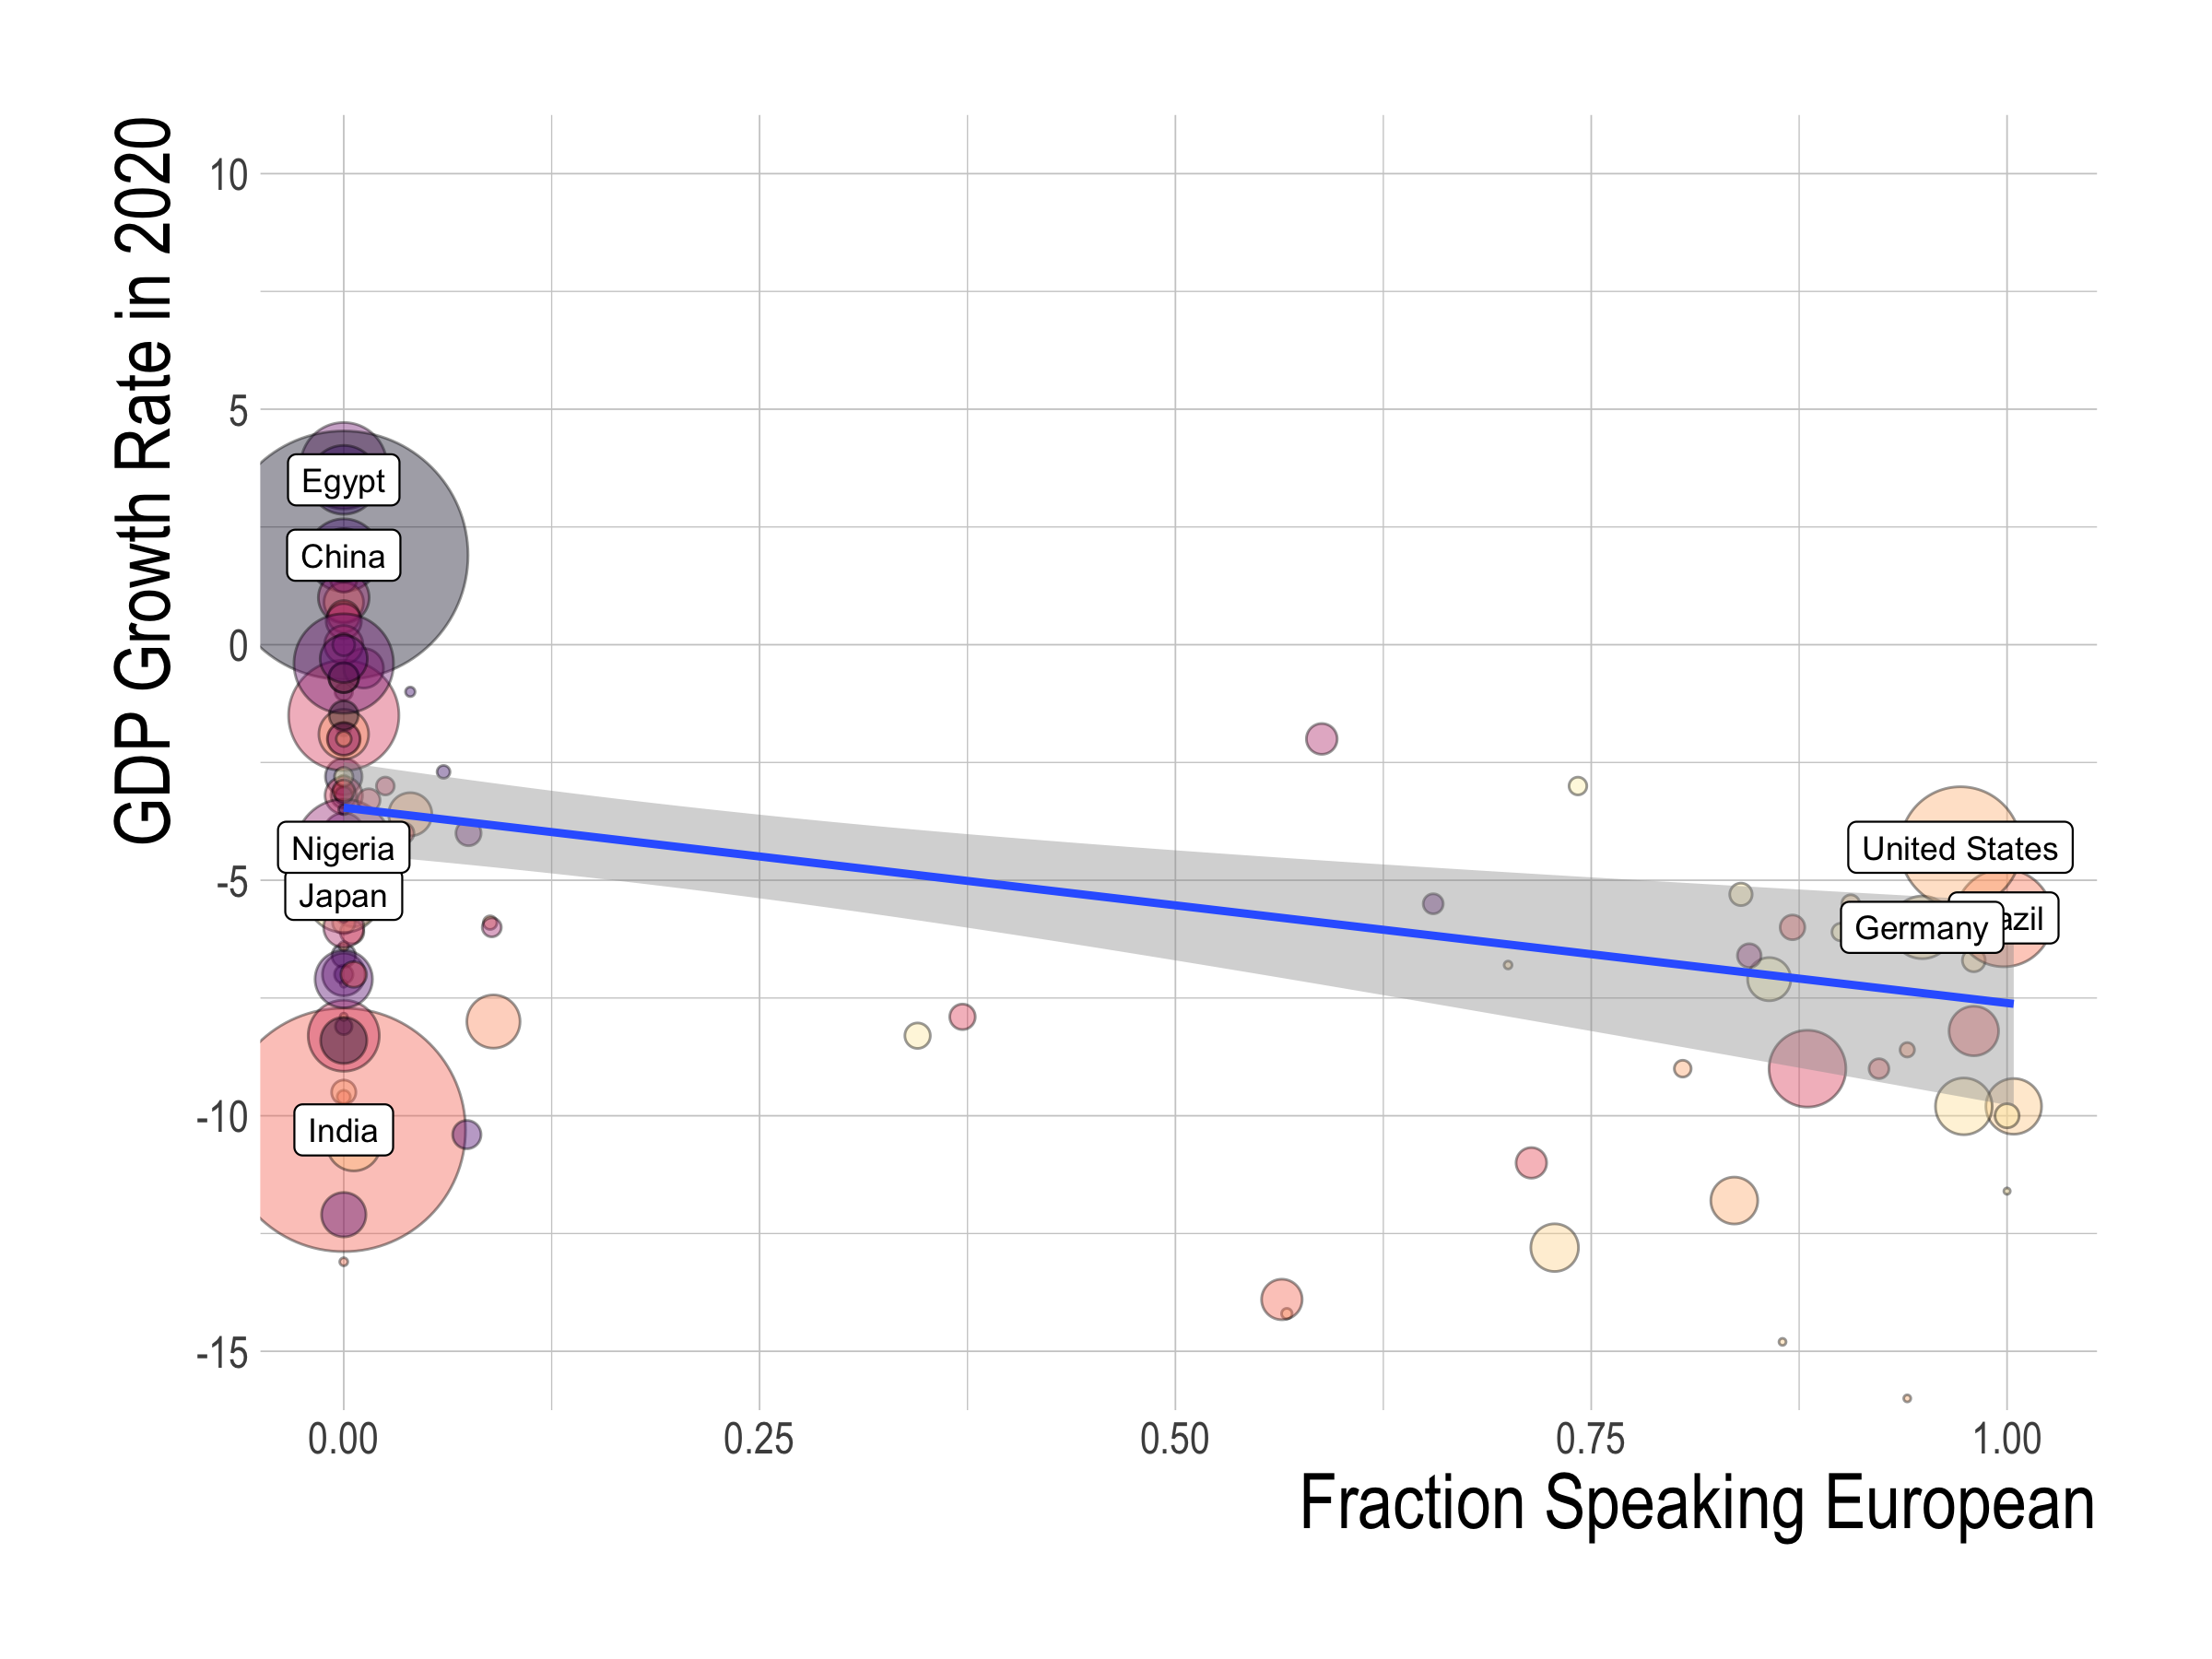
\includegraphics[width=5in]{plots/gdp_eurfrac_noControls_popWeighted_ols.png}}\hspace{1em}%
    \subcaptionbox{Total Covid-19-related Deaths Per Million\label{fig:reduced-deaths-eurfrac}}{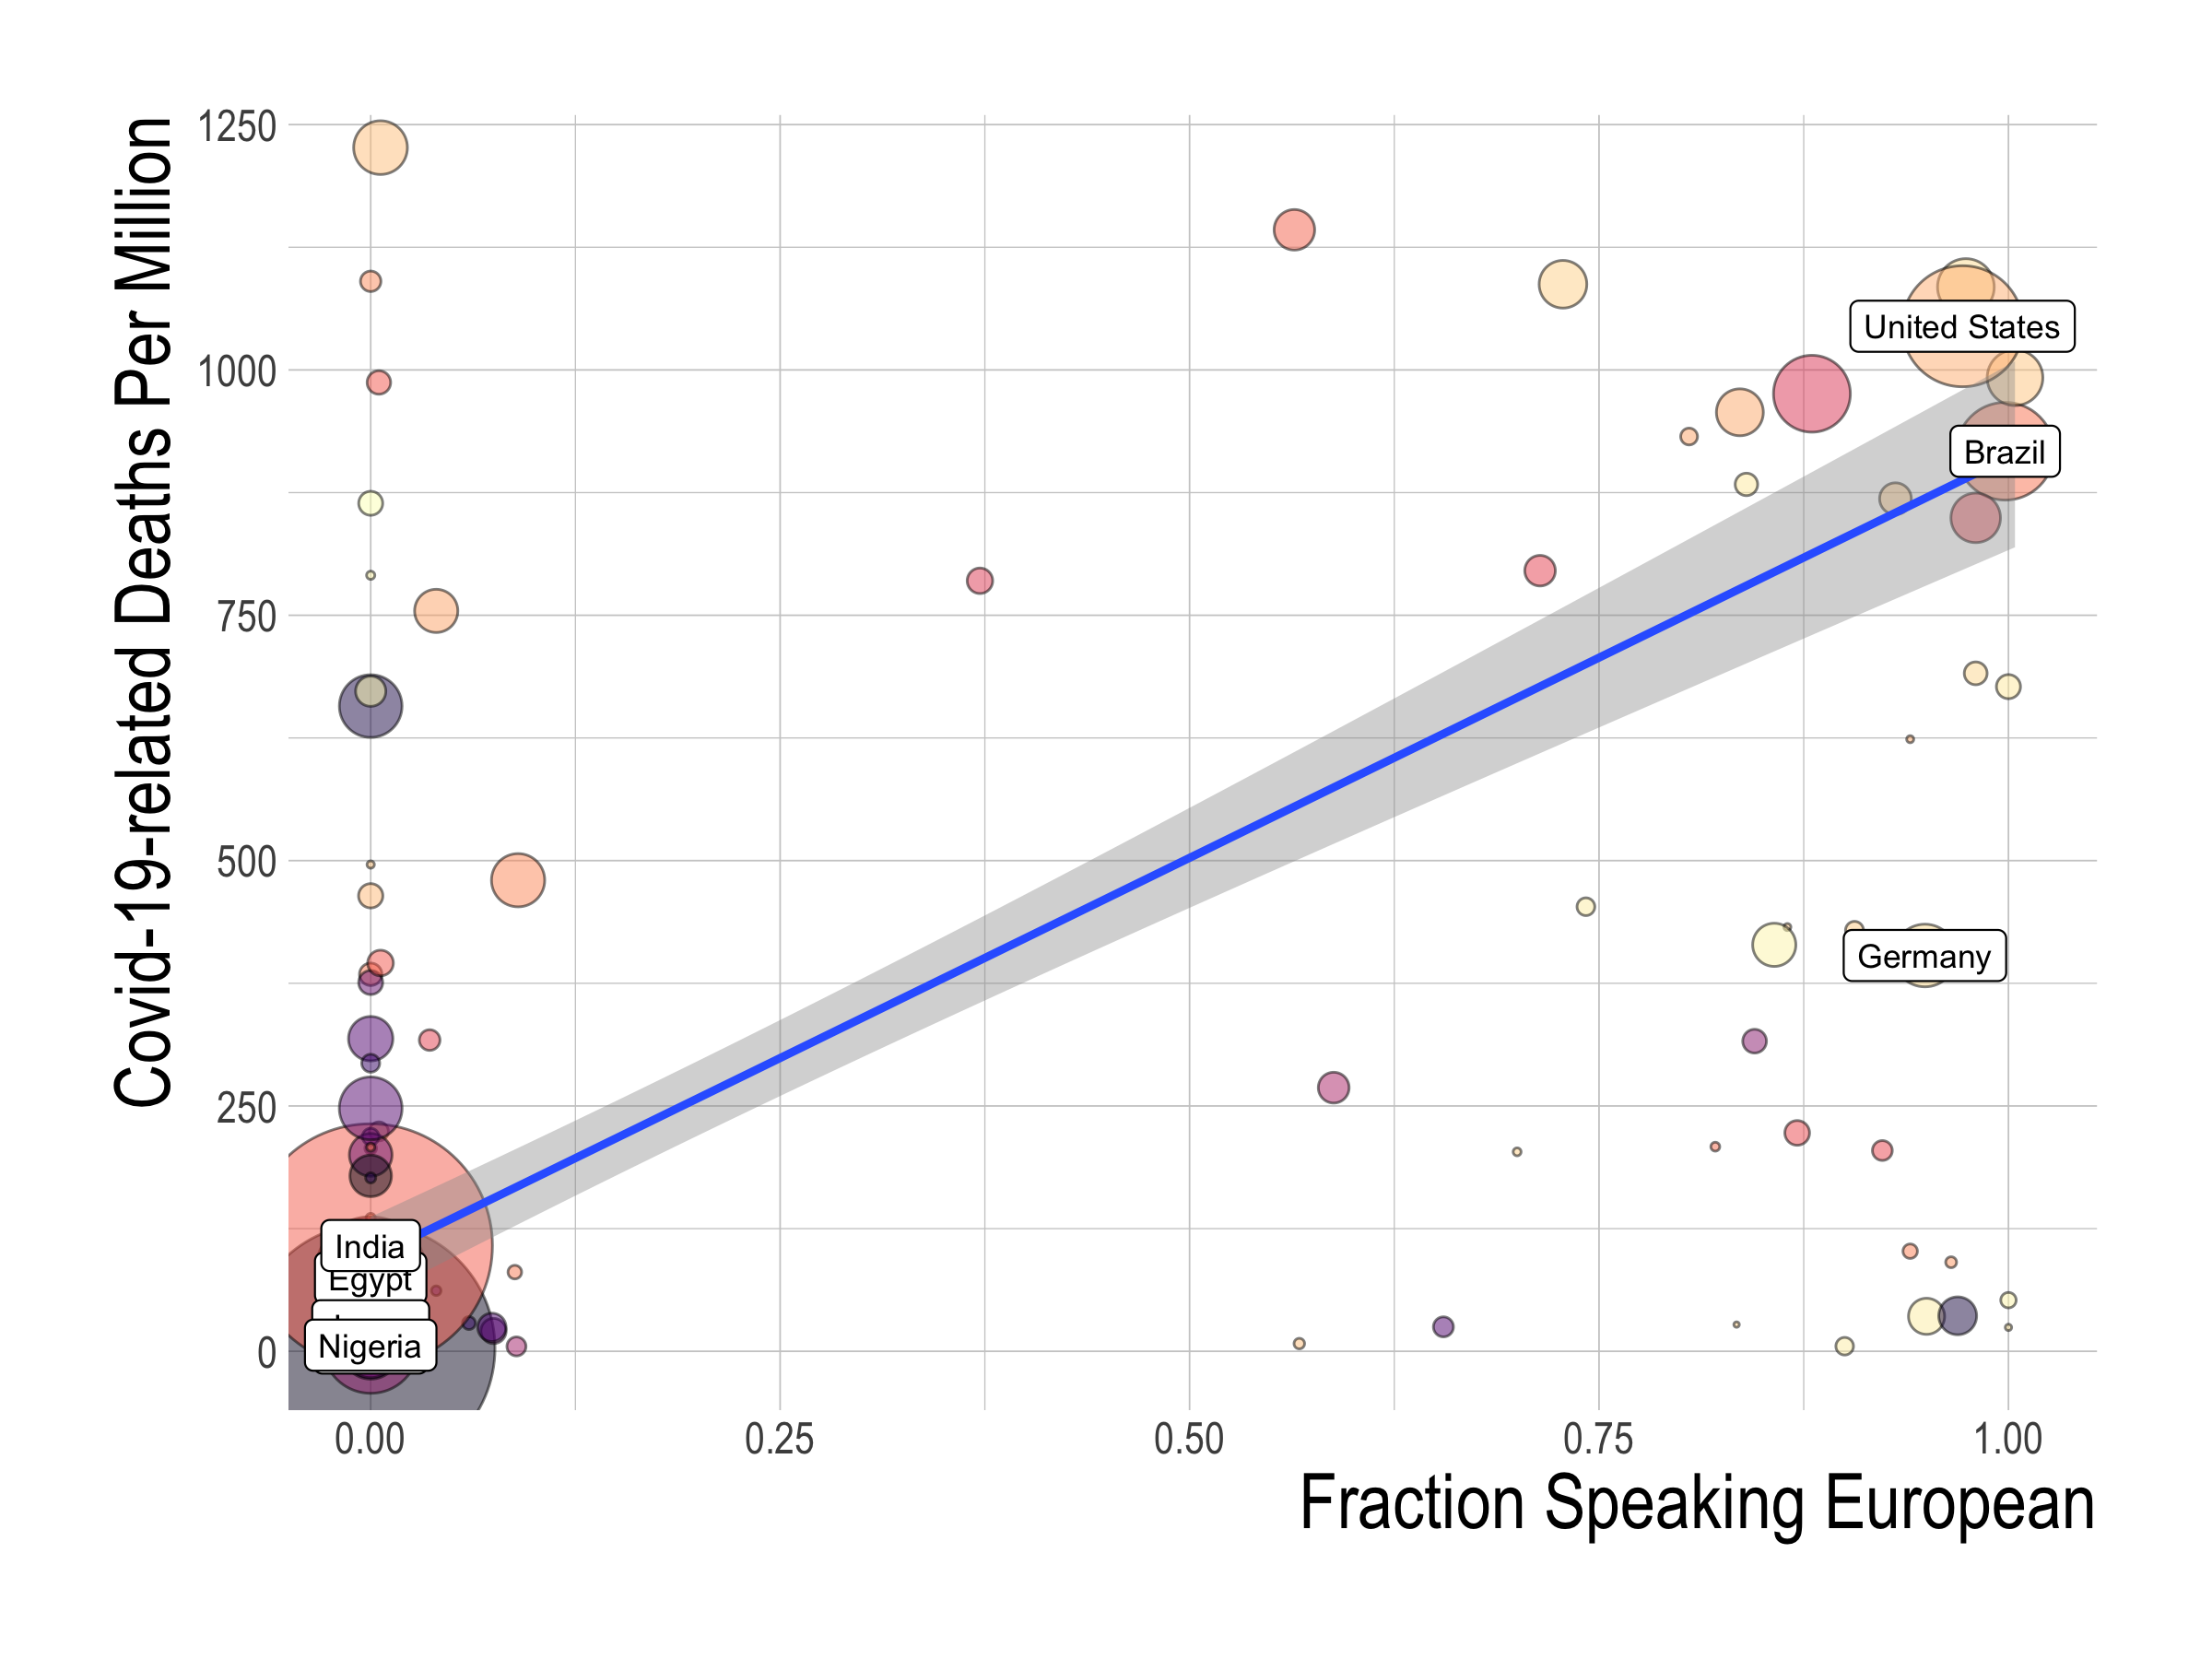
\includegraphics[width=5in]{plots/deaths_eurfrac_noControls_popWeighted_ols.png}}\hspace{1em}%
  
  \caption*{\textit{Notes:} The size of each observation point is proportional to the size of the population of each country. The colors vary depending on the level of the Democracy Index (Freedom House). The regression line corresponds to the reduced-form OLS regression without controls and weighted by population. The shaded area corresponds to the 95\% confidence interval.}
  
\end{figure}
% \begin{figure}[!htbp]
\centering
\caption{Reduced Form Relationship Between Covid-19-related Outcomes and Population Density in 1500}
\centering
\label{fig:reduced-form-lpd}
  \subcaptionbox{GDP Growth Rates in 2020 \label{fig:reduced-gdp-lpd}}{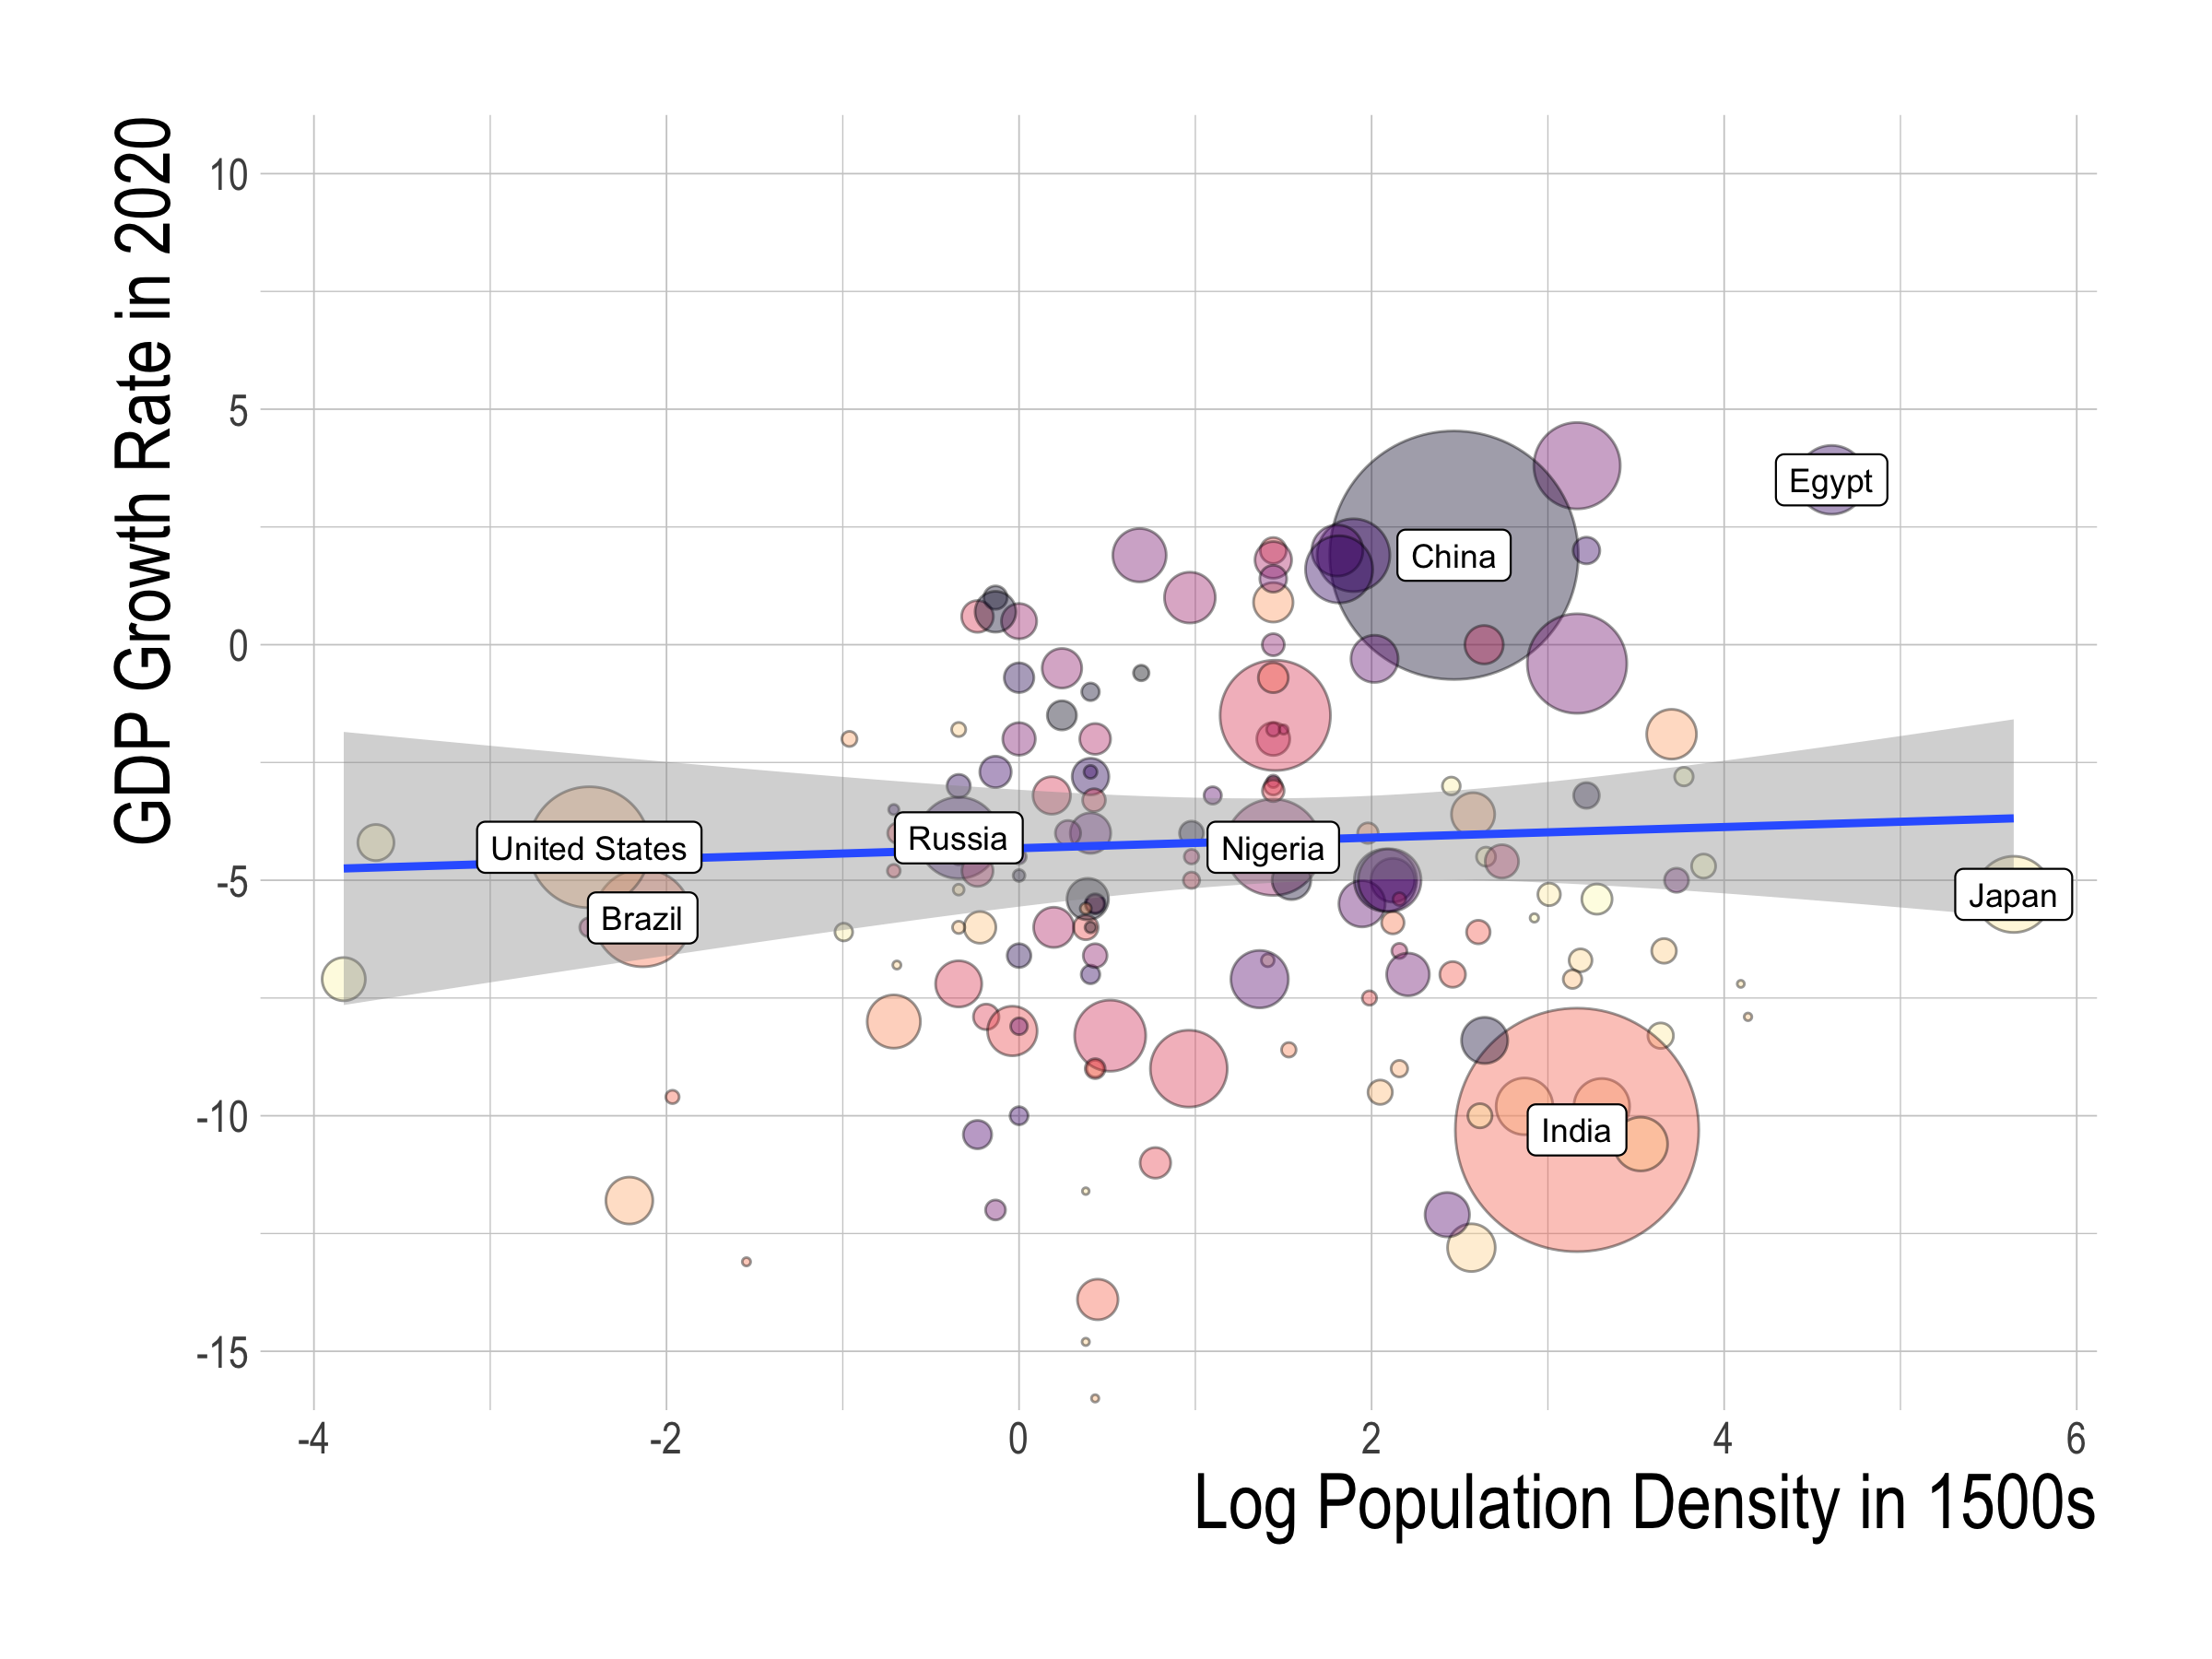
\includegraphics[width=5in]{plots/gdp_lpd1500s_noControls_popWeighted_ols.png}}
      \subcaptionbox{Total Covid-19-related Deaths Per Million\label{fig:reduced-deaths-lpd}}{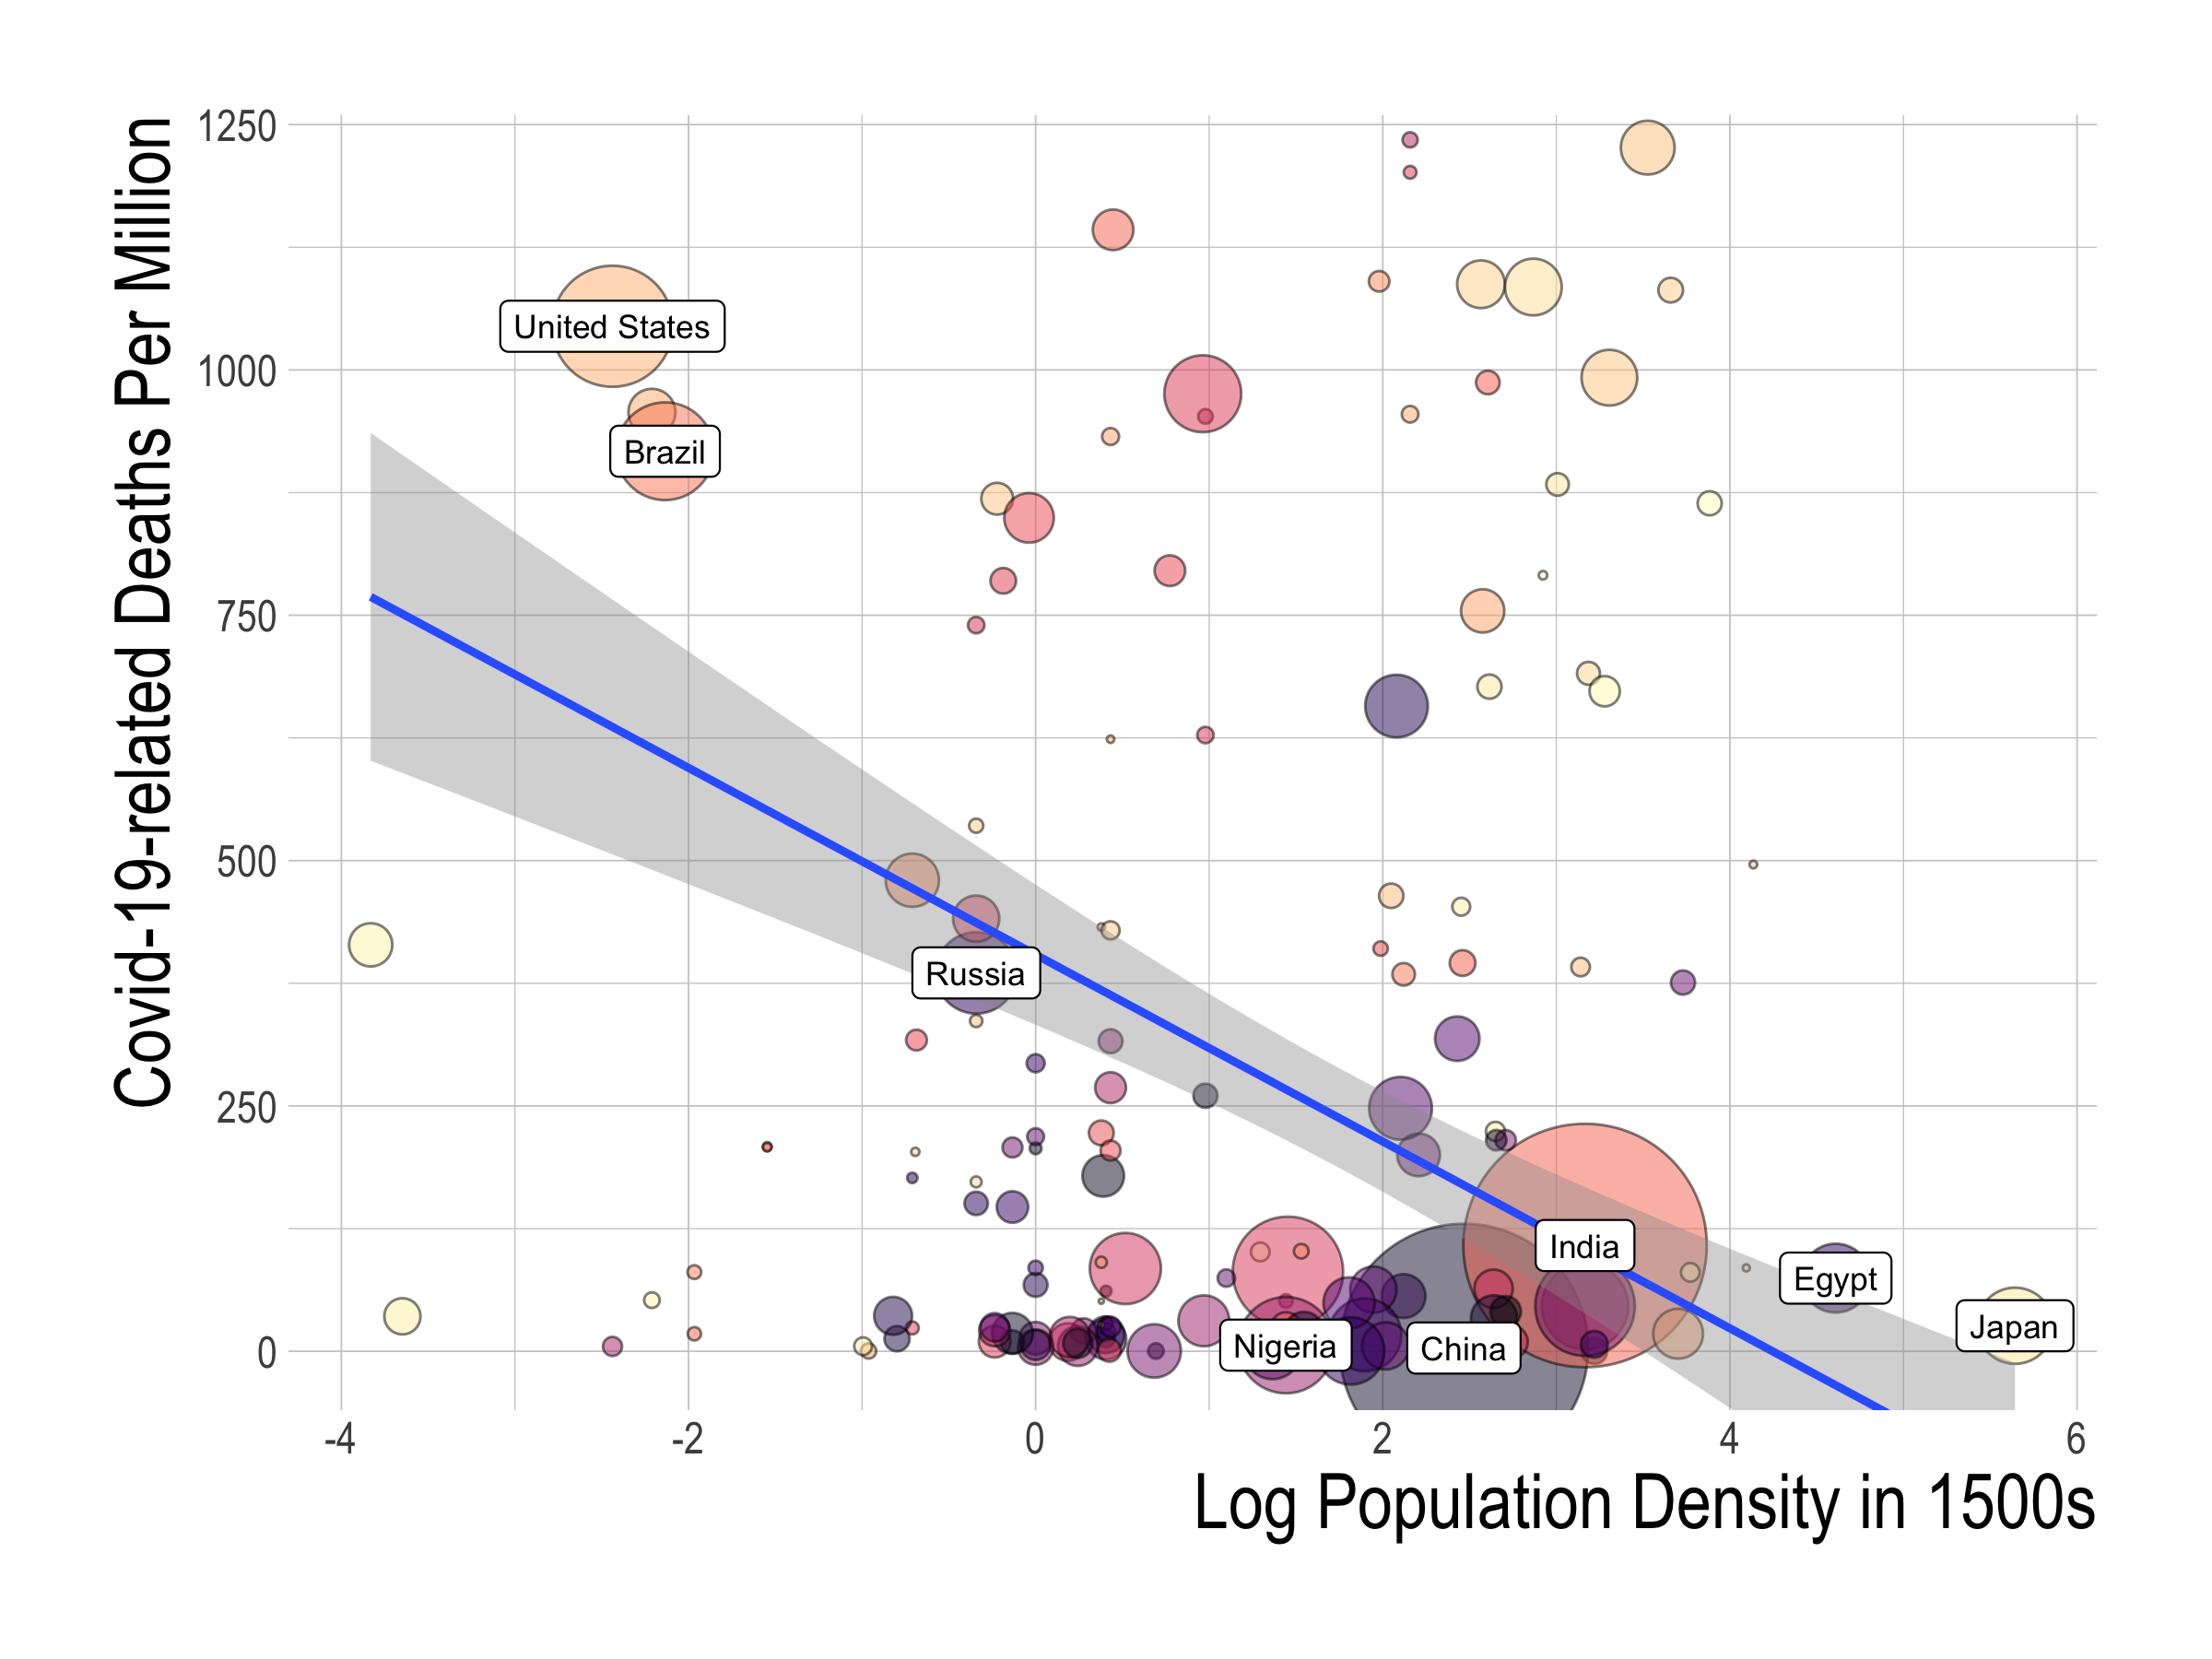
\includegraphics[width=5in]{plots/deaths_lpd1500s_noControls_popWeighted_ols.png}}
  \caption*{\textit{Notes:} The size of each observation point is proportional to the size of the population of each country. The colors vary depending on the level of the Democracy Index (Freedom House). The regression line corresponds to the reduced-form OLS regression without controls and weighted by population. The shaded area corresponds to the 95\% confidence interval.}
  
\end{figure}

% \newpage
% \setcounter{table}{0}
% \subsection{Use the Same Sample among Different IVs}
% 
\begin{table}[!htbp] 
  \caption{2SLS Regressions on GDP Growth Rates in 2020}
  \label{tab:2sls-gdp-restrict-sample} 
  \footnotesize
  \begin{threeparttable}
\begin{tabular}{@{\extracolsep{0pt}}lcccccccccc} 
\\[-1.8ex]\hline 
\hline \\[-1.8ex] 
 & \multicolumn{10}{c}{\textit{Dependent variable:}} \\ 
\cline{2-11} 
\\[-1.8ex] & \multicolumn{10}{c}{GDP Growth Rates in 2020} \\ 
\\[-1.8ex] & (1) & (2) & (3) & (4) & (5) & (6) & (7) & (8) & (9) & (10)\\ 
\hline \\[-1.8ex] 
  & \multicolumn{10}{c}{Panel A: Two-Stage Least Squares} \\
   Democracy Index & $-$4.4$^{***}$ & $-$3.8$^{***}$ & $-$2.6 & $-$3.2$^{***}$ & $-$4.6$^{***}$ & $-$3.6$^{***}$ & $-$2.5 & $-$4.8$^{***}$ & $-$1.3 & $-$2.5$^{**}$ \\ 
 (Freedom House) & (1.4) & (1.1) & (1.7) & (0.9) & (0.9) & (0.9) & (3.2) & (1.4) & (3.3) & (1.1) \\ 
 \hline \\[-1.8ex] 
   & \multicolumn{10}{c}{Panel B: First Stage for the Democracy Index (Freedom House)} \\
  Log European Settler Mortality & $-$0.4$^{**}$ & $-$0.5$^{***}$ &  &  &  &  &  &  &  &  \\ 
  & (0.2) & (0.2) &  &  &  &  &  &  &  &  \\ 
  Fraction Speaking English &  &  & 0.8$^{***}$ & 1.4$^{***}$ &  &  &  &  &  &  \\ 
  &  &  & (0.2) & (0.4) &  &  &  &  &  &  \\ 
  Fraction Speaking European &  &  & 1.0$^{**}$ & 0.9$^{***}$ &  &  &  &  &  &  \\ 
  &  &  & (0.4) & (0.3) &  &  &  &  &  &  \\ 
  Frankel-Romer Trade Share &  &  & 0.2 & $-$0.3 &  &  &  &  &  &  \\ 
  &  &  & (0.4) & (0.2) &  &  &  &  &  &  \\ 
  British Legal Origin &  &  &  &  & 1.7$^{***}$ & 2.5$^{***}$ &  &  &  &  \\ 
  &  &  &  &  & (0.2) & (0.2) &  &  &  &  \\ 
  French Legal Origin &  &  &  &  & 1.4$^{***}$ & 2.2$^{***}$ &  &  &  &  \\ 
  &  &  &  &  & (0.2) & (0.2) &  &  &  &  \\ 
  Bananas &  &  &  &  &  &  & $-$0.1 & $-$0.1 &  &  \\ 
  &  &  &  &  &  &  & (0.4) & (0.2) &  &  \\ 
  Coffee &  &  &  &  &  &  & 0.5 & 1.4$^{***}$ &  &  \\ 
  &  &  &  &  &  &  & (0.4) & (0.4) &  &  \\ 
  Maize &  &  &  &  &  &  & 1.4$^{*}$ & 2.1$^{***}$ &  &  \\ 
  &  &  &  &  &  &  & (0.8) & (0.8) &  &  \\ 
  Millet &  &  &  &  &  &  & $-$0.2 & 0.8$^{**}$ &  &  \\ 
  &  &  &  &  &  &  & (0.5) & (0.3) &  &  \\ 
  Rice &  &  &  &  &  &  & $-$0.6 & $-$2.6$^{***}$ &  &  \\ 
  &  &  &  &  &  &  & (0.6) & (1.0) &  &  \\ 
  Sugar &  &  &  &  &  &  & $-$0.7 & $-$0.6 &  &  \\ 
  &  &  &  &  &  &  & (0.7) & (0.6) &  &  \\ 
  Rubber &  &  &  &  &  &  & $-$0.5 & $-$1.3$^{***}$ &  &  \\ 
  &  &  &  &  &  &  & (0.6) & (0.4) &  &  \\ 
  Wheat &  &  &  &  &  &  & $-$0.1 & 0.001 &  &  \\ 
  &  &  &  &  &  &  & (0.4) & (0.3) &  &  \\ 
  Log Population Density in 1500s &  &  &  &  &  &  &  &  & $-$0.2 & $-$0.3$^{***}$ \\ 
  &  &  &  &  &  &  &  &  & (0.1) & (0.1) \\ 
R$^{2}$ & 0.2 & 0.6 & 0.3 & 0.7 & 0.6 & 0.8 & 0.1 & 0.7 & 0.1 & 0.6 \\ 
F Statistic & 19.0$^{***}$ & 12.7$^{***}$ & 11.0$^{***}$ & 16.8$^{***}$ & 50.5$^{***}$ & 28.9$^{***}$ & 1.0 & 9.6$^{***}$ & 11.0$^{***}$ & 13.1$^{***}$ \\ 

 \hline \\[-1.8ex] 
   & \multicolumn{10}{c}{Panel C: Ordinary Least Squares} \\
Democracy Index & $-$4.0$^{***}$ & $-$3.5$^{***}$ & $-$4.0$^{***}$ & $-$3.5$^{***}$ & $-$4.0$^{***}$ & $-$3.5$^{***}$ & $-$4.0$^{***}$ & $-$3.5$^{***}$ & $-$4.0$^{***}$ & $-$3.5$^{***}$ \\ 
 (Freedom House)  & (0.8) & (0.8) & (0.8) & (0.8) & (0.8) & (0.8) & (0.8) & (0.8) & (0.5) & (0.5) \\ 
R$^{2}$ & 0.5 & 0.6 & 0.5 & 0.6 & 0.5 & 0.6 & 0.5 & 0.6 & 0.5 & 0.6 \\ 
  \hline \\[-1.8ex] 
Weighting & Pop & Pop & Pop & Pop & Pop & Pop & Pop & Pop & Pop & Pop \\ 
Controls & \xmark & \cmark & \xmark & \cmark & \xmark & \cmark & \xmark & \cmark & \xmark & \cmark\\ 
N & 78 & 78 & 78 & 78 & 78 & 78 & 78 & 78 & 78 & 78 \\ 
\hline 
\hline \\[-1.8ex] 
  & \multicolumn{10}{r}{$^{*}$p$<$0.1; $^{**}$p$<$0.05; $^{***}$p$<$0.01} \\ 
\end{tabular} 
\begin{tablenotes} 
\item {\footnotesize {\textit{Notes:}  The Democracy Index (Freedom House) is the sum of the political rights and civil liberties scales from Freedom in the World 2020 by Freedom House and has been normalized by its standard deviation. Panel A reports the two-stage least squares estimates of the effect of democracy on GDP growth rates in 2020, using five different instrumental variable strategies. Panel B reports the corresponding first stage regressions. Panel C reports the coefficients from an OLS regression of GDP growth rates in 2020 against the Freedom House index. Columns (1), (3), (5), (7) and (9) have no controls, while columns (2), (4), (6), (8) and (10) have the following controls: absolute latitude, mean temperature, mean precipitation, population density, median age and diabetes prevalence. All regressions have been weighted by population. Robust standard errors are in parentheses. }}
\end{tablenotes}
\end{threeparttable}
\end{table} 


% 
\begin{table}[!htbp] \centering
  \caption{2SLS Regressions on Covid-19-related Deaths Per Million}
  \label{tab:2sls-deaths-restrict-sample} 
  \footnotesize
  \begin{threeparttable}
\begin{tabular}{@{\extracolsep{0pt}}lcccccccccc} 
\\[-1.8ex]\hline 
\hline \\[-1.8ex] 
 & \multicolumn{10}{c}{\textit{Dependent variable:}} \\ 
\cline{2-11} 
\\[-1.8ex] & \multicolumn{10}{c}{Covid-19-related Deaths Per Million} \\ 
\\[-1.8ex] & (1) & (2) & (3) & (4) & (5) & (6) & (7) & (8) & (9) & (10)\\ 
\hline \\[-1.8ex] 
  & \multicolumn{10}{c}{Panel A: Two-Stage Least Squares} \\
Democracy index & 428.1$^{***}$ & 394.7$^{***}$ & 566.4$^{**}$ & 475.6$^{***}$ & 145.5$^{**}$ & 368.9$^{***}$ & 443.9 & 263.8$^{***}$ & 678.0$^{*}$ & 532.9$^{***}$ \\ 
(Freedom House)  & (151.8) & (66.9) & (242.3) & (71.1) & (66.7) & (56.4) & (316.2) & (95.0) & (390.8) & (140.0) \\ 
\hline \\[-1.8ex] 
   & \multicolumn{10}{c}{Panel B: First Stage for the Democracy Index (Freedom House)} \\
  Log European Settler Mortality & $-$0.4$^{**}$ & $-$0.5$^{***}$ &  &  &  &  &  &  &  &  \\ 
  & (0.2) & (0.2) &  &  &  &  &  &  &  &  \\ 
  Fraction Speaking English &  &  & 0.8$^{***}$ & 1.4$^{***}$ &  &  &  &  &  &  \\ 
  &  &  & (0.2) & (0.4) &  &  &  &  &  &  \\ 
  Fraction Speaking European &  &  & 1.0$^{**}$ & 0.9$^{***}$ &  &  &  &  &  &  \\ 
  &  &  & (0.4) & (0.3) &  &  &  &  &  &  \\ 
  Frankel-Romer Trade Share &  &  & 0.2 & $-$0.3 &  &  &  &  &  &  \\ 
  &  &  & (0.4) & (0.2) &  &  &  &  &  &  \\ 
  British Legal Origin &  &  &  &  & 1.7$^{***}$ & 2.5$^{***}$ &  &  &  &  \\ 
  &  &  &  &  & (0.2) & (0.2) &  &  &  &  \\ 
  French Legal Origin &  &  &  &  & 1.4$^{***}$ & 2.2$^{***}$ &  &  &  &  \\ 
  &  &  &  &  & (0.2) & (0.2) &  &  &  &  \\ 
  Bananas &  &  &  &  &  &  & $-$0.1 & $-$0.1 &  &  \\ 
  &  &  &  &  &  &  & (0.4) & (0.2) &  &  \\ 
  Coffee &  &  &  &  &  &  & 0.5 & 1.4$^{***}$ &  &  \\ 
  &  &  &  &  &  &  & (0.4) & (0.4) &  &  \\ 
  Maize &  &  &  &  &  &  & 1.4$^{*}$ & 2.1$^{***}$ &  &  \\ 
  &  &  &  &  &  &  & (0.8) & (0.8) &  &  \\ 
  Millet &  &  &  &  &  &  & $-$0.2 & 0.8$^{**}$ &  &  \\ 
  &  &  &  &  &  &  & (0.5) & (0.3) &  &  \\ 
  Rice &  &  &  &  &  &  & $-$0.6 & $-$2.6$^{***}$ &  &  \\ 
  &  &  &  &  &  &  & (0.6) & (1.0) &  &  \\ 
  Sugarcane &  &  &  &  &  &  & $-$0.7 & $-$0.6 &  &  \\ 
  &  &  &  &  &  &  & (0.7) & (0.6) &  &  \\ 
  Rubber &  &  &  &  &  &  & $-$0.5 & $-$1.3$^{***}$ &  &  \\ 
  &  &  &  &  &  &  & (0.6) & (0.4) &  &  \\ 
  Wheat &  &  &  &  &  &  & $-$0.1 & 0.001 &  &  \\ 
  &  &  &  &  &  &  & (0.4) & (0.3) &  &  \\ 
  Log Population Density in 1500s &  &  &  &  &  &  &  &  & $-$0.2 & $-$0.3$^{***}$ \\ 
  &  &  &  &  &  &  &  &  & (0.1) & (0.1) \\ 
R$^{2}$ & 0.2 & 0.6 & 0.3 & 0.7 & 0.6 & 0.8 & 0.1 & 0.7 & 0.1 & 0.6 \\ 
F Statistic & 19.0$^{***}$ & 12.7$^{***}$ & 11.0$^{***}$ & 16.8$^{***}$ & 50.5$^{***}$& 28.9$^{***}$ & 1.0 & 9.6$^{***}$ & 11.0$^{***}$ & 13.1$^{***}$\\ 
% F Statistic & 20.2$^{***}$ (df = 1; 82) & 10.8$^{***}$ (df = 7; 76) & 11.5$^{***}$ (df = 3; 77) & 17.5$^{***}$ (df = 9; 71) & 48.2$^{***}$ (df = 2; 81) & 23.5$^{***}$ (df = 8; 75) & 1.1 (df = 8; 75) & 7.3$^{***}$ (df = 14; 69) & 11.3$^{***}$ (df = 1; 79) & 11.2$^{***}$ (df = 7; 73) \\ 
 
 \hline \\[-1.8ex] 
  & \multicolumn{10}{c}{Panel C: Ordinary Least Squares} \\
 Democracy Index (Freedom House) & 220.0$^{***}$ & 284.1$^{***}$ & 220.0$^{***}$ & 284.1$^{***}$ & 220.0$^{***}$ & 284.1$^{***}$ & 220.0$^{***}$ & 284.1$^{***}$ & 220.0$^{***}$ & 284.1$^{***}$ \\ 
 (Freedom House) & (78.9) & (65.5) & (78.9) & (65.5) & (78.9) & (65.5) & (78.9) & (65.5) & (34.5) & (37.5) \\
  \hline \\[-1.8ex] 
Weighting & Pop & Pop & Pop & Pop & Pop & Pop & Pop & Pop & Pop & Pop \\ 
Controls & \xmark & \cmark & \xmark & \cmark & \xmark & \cmark & \xmark & \cmark & \xmark & \cmark\\ 
N  & 78 & 78 & 78 & 78 & 78 & 78 & 78 & 78 & 78 & 78 \\ 
\hline 
\hline \\[-1.8ex] 
 & \multicolumn{10}{r}{$^{*}$p$<$0.1; $^{**}$p$<$0.05; $^{***}$p$<$0.01} \\ 
\end{tabular} 
\begin{tablenotes} 
\item {\footnotesize {\textit{Notes:} The Democracy Index (Freedom House) is the sum of the political rights and civil liberties scales from Freedom in the World 2020 by Freedom House and has been normalized by its standard deviation. Panel A reports the two-stage least squares estimates of the effect of democracy on Covid-19-related deaths per million, using five different instrumental variable strategies. Panel B reports the corresponding first stage regressions. Panel C reports the coefficients from an OLS regression of Covid-19-related deaths per million against the Freedom House index.  Columns (1), (3), (5), (7) and (9) have no controls, while columns (2), (4), (6), (8) and (10) have the following controls: absolute latitude, mean temperature, mean precipitation, population density, median age and diabetes prevalence. All regressions have been weighted by population.}}
\end{tablenotes}
\end{threeparttable}
\end{table} 


% \newpage
% \setcounter{table}{0}
% \subsection{Exclude US and China from Sample}
% 
\begin{table}[!htbp] 
  \caption{2SLS Regressions on GDP Growth Rates in 2020}
  \label{tab:2sls-gdp-exclude-US-China} 
  \footnotesize
  \begin{threeparttable}
\begin{tabular}{@{\extracolsep{0pt}}lcccccccccc} 
\\[-1.8ex]\hline 
\hline \\[-1.8ex] 
 & \multicolumn{10}{c}{\textit{Dependent variable:}} \\ 
\cline{2-11} 
\\[-1.8ex] & \multicolumn{10}{c}{GDP Growth Rates in 2020} \\ 
\\[-1.8ex] & (1) & (2) & (3) & (4) & (5) & (6) & (7) & (8) & (9) & (10)\\ 
\hline \\[-1.8ex] 

  & \multicolumn{10}{c}{Panel A: Two-Stage Least Squares} \\
 Democracy Index  & $-$6.4$^{***}$ & $-$7.3 & $-$5.2$^{***}$ & $-$5.6$^{***}$ & $-$3.5 & $-$4.9$^{**}$ & $-$6.1$^{***}$ & $-$7.0$^{***}$ & $-$3.0 & 5.2 \\ 
 (Freedom House) & (1.8) & (9.6) & (1.3) & (1.3) & (5.8) & (2.2) & (2.1) & (1.6) & (7.3) & (14.7) \\ 
 \hline \\[-1.8ex] 
 
 
   & \multicolumn{10}{c}{Panel B: First Stage for the Democracy Index (Freedom House)} \\
  Log European Settler Mortality & $-$0.2$^{***}$ & $-$0.1 &  &  &  &  &  &  &  &  \\ 
  & (0.1) & (0.1) &  &  &  &  &  &  &  &  \\ 
  Fraction Speaking English &  &  & 0.9$^{***}$ & 0.05 &  &  &  &  &  &  \\ 
  &  &  & (0.3) & (0.2) &  &  &  &  &  &  \\ 
  Fraction Speaking European &  &  & 0.7$^{***}$ & 0.3$^{*}$ &  &  &  &  &  &  \\ 
  &  &  & (0.3) & (0.2) &  &  &  &  &  &  \\ 
  Frankel-Romer Trade Share &  &  & $-$0.3$^{**}$ & $-$0.5$^{***}$ &  &  &  &  &  &  \\ 
  &  &  & (0.1) & (0.1) &  &  &  &  &  &  \\ 
  British Legal Origin &  &  &  &  & $-$0.01 & 0.9$^{***}$ &  &  &  &  \\ 
  &  &  &  &  & (0.5) & (0.3) &  &  &  &  \\ 
  French Legal Origin &  &  &  &  & $-$0.3 & 0.4 &  &  &  &  \\ 
  &  &  &  &  & (0.5) & (0.3) &  &  &  &  \\ 
  Bananas &  &  &  &  &  &  & 0.2 & 0.1 &  &  \\ 
  &  &  &  &  &  &  & (0.2) & (0.2) &  &  \\ 
  Coffee &  &  &  &  &  &  & 0.03 & 0.4 &  &  \\ 
  &  &  &  &  &  &  & (0.3) & (0.3) &  &  \\ 
  Maize &  &  &  &  &  &  & 0.5 & 0.2 &  &  \\ 
  &  &  &  &  &  &  & (0.5) & (0.4) &  &  \\ 
  Millet &  &  &  &  &  &  & $-$0.3 & $-$0.01 &  &  \\ 
  &  &  &  &  &  &  & (0.2) & (0.2) &  &  \\ 
  Rice &  &  &  &  &  &  & $-$0.4 & $-$0.3 &  &  \\ 
  &  &  &  &  &  &  & (0.4) & (0.3) &  &  \\ 
  Sugar &  &  &  &  &  &  & $-$0.4 & 0.1 &  &  \\ 
  &  &  &  &  &  &  & (0.4) & (0.3) &  &  \\ 
  Rubber &  &  &  &  &  &  & 0.5$^{*}$ & 0.2 &  &  \\ 
  &  &  &  &  &  &  & (0.3) & (0.2) &  &  \\ 
  Wheat &  &  &  &  &  &  & 0.6$^{**}$ & 0.5 &  &  \\ 
  &  &  &  &  &  &  & (0.2) & (0.4) &  &  \\ 
  Log Population Density in 1500s &  &  &  &  &  &  &  &  & 0.1 & 0.04 \\ 
  &  &  &  &  &  &  &  &  & (0.1) & (0.1) \\ 
R$^{2}$ & 0.1 & 0.3 & 0.3 & 0.6 & 0.03 & 0.4 & 0.2 & 0.4 & 0.02 & 0.3 \\ 
F Statistic & 13.1$^{***}$ & 4.7$^{***}$ & 15.3$^{***}$ & 22.2$^{***}$ & 2.0 & 11.5$^{***}$ & 3.4$^{***}$ & 8.3$^{***}$ & 2.4 & 9.6$^{***}$ \\

 \hline \\[-1.8ex] 
   & \multicolumn{10}{c}{Panel C: Ordinary Least Squares} \\
Democracy Index & $-$4.3$^{***}$ & $-$4.2$^{***}$ & $-$2.8$^{***}$ & $-$3.3$^{***}$ & $-$2.7$^{***}$ & $-$2.8$^{***}$ & $-$2.6$^{***}$ & $-$2.7$^{***}$ & $-$2.7$^{***}$ & $-$2.7$^{***}$ \\ 
 (Freedom House)  & (1.2) & (1.3) & (0.9) & (1.3) & (0.9) & (1.0) & (0.8) & (1.0) & (0.5) & (0.6) \\ 
R$^{2}$ & 0.3 & 0.5 & 0.2 & 0.4 & 0.2 & 0.3 & 0.2 & 0.3 & 0.2 & 0.3 \\ 
  \hline \\[-1.8ex] 
Weighting & Pop & Pop & Pop & Pop & Pop & Pop & Pop & Pop & Pop & Pop \\ 
Controls & \xmark & \cmark & \xmark & \cmark & \xmark & \cmark & \xmark & \cmark & \xmark & \cmark\\ 
N & 82 & 82 & 127 & 127 & 151 & 151 & 159 & 159 & 151 & 151 \\ 
\hline 
\hline \\[-1.8ex] 
  & \multicolumn{10}{r}{$^{*}$p$<$0.1; $^{**}$p$<$0.05; $^{***}$p$<$0.01} \\ 
\end{tabular} 
\begin{tablenotes} 
\item {\footnotesize {\textit{Notes:}  The Democracy Index (Freedom House) is the sum of the political rights and civil liberties scales from Freedom in the World 2020 by Freedom House and has been normalized by its standard deviation. Panel A reports the two-stage least squares estimates of the effect of democracy on GDP growth rates in 2020, using five different instrumental variable strategies. Panel B reports the corresponding first stage regressions. Panel C reports the coefficients from an OLS regression of GDP growth rates in 2020 against the Freedom House index. Columns (1), (3), (5), (7) and (9) have no controls, while columns (2), (4), (6), (8) and (10) have the following controls: absolute latitude, mean temperature, mean precipitation, population density, median age and diabetes prevalence. All regressions have been weighted by population. Robust standard errors are in parentheses. }}
\end{tablenotes}
\end{threeparttable}
\end{table} 


% 
\begin{table}[!htbp] \centering
  \caption{2SLS Regressions on Covid-19-related Deaths Per Million}
  \label{tab:2sls-deaths-exclude-US-China} 
  \footnotesize
  \begin{threeparttable}
\begin{tabular}{@{\extracolsep{0pt}}lcccccccccc} 
\\[-1.8ex]\hline 
\hline \\[-1.8ex] 
 & \multicolumn{10}{c}{\textit{Dependent variable:}} \\ 
\cline{2-11} 
\\[-1.8ex] & \multicolumn{10}{c}{Covid-19-related Deaths Per Million} \\ 
\\[-1.8ex] & (1) & (2) & (3) & (4) & (5) & (6) & (7) & (8) & (9) & (10)\\ 
\hline \\[-1.8ex] 
  & \multicolumn{10}{c}{Panel A: Two-Stage Least Squares} \\
Democracy Index& 459.8$^{**}$ & 769.0 & 435.2$^{***}$ & 172.9 & $-$900.7 & $-$54.0 & 246.4 & 108.3 & $-$912.1 & $-$1,605.3 \\ 
 (Freedom House)   & (179.9) & (1,355.1) & (161.1) & (164.5) & (977.6) & (160.6) & (224.3) & (133.3) & (1,540.1) & (2,456.5) \\ 
\hline \\[-1.8ex] 
   & \multicolumn{10}{c}{Panel B: First Stage for the Democracy Index (Freedom House)} \\
  Log European Settler Mortality & $-$0.2$^{***}$ & $-$0.1 &  &  &  &  &  &  &  &  \\ 
  & (0.1) & (0.1) &  &  &  &  &  &  &  &  \\ 
  Fraction Speaking English &  &  & 0.9$^{***}$ & 0.05 &  &  &  &  &  &  \\ 
  &  &  & (0.3) & (0.2) &  &  &  &  &  &  \\ 
  Fraction Speaking European &  &  & 0.7$^{***}$ & 0.3$^{*}$ &  &  &  &  &  &  \\ 
  &  &  & (0.3) & (0.2) &  &  &  &  &  &  \\ 
  Frankel-Romer Trade Share &  &  & $-$0.3$^{**}$ & $-$0.5$^{***}$ &  &  &  &  &  &  \\ 
  &  &  & (0.1) & (0.1) &  &  &  &  &  &  \\ 
  British Legal Origin &  &  &  &  & $-$0.01 & 0.9$^{***}$ &  &  &  &  \\ 
  &  &  &  &  & (0.5) & (0.3) &  &  &  &  \\ 
  French Legal Origin &  &  &  &  & $-$0.3 & 0.4 &  &  &  &  \\ 
  &  &  &  &  & (0.5) & (0.3) &  &  &  &  \\ 
  Bananas &  &  &  &  &  &  & 0.2 & 0.1 &  &  \\ 
  &  &  &  &  &  &  & (0.2) & (0.2) &  &  \\ 
  Coffee &  &  &  &  &  &  & 0.03 & 0.4 &  &  \\ 
  &  &  &  &  &  &  & (0.3) & (0.3) &  &  \\ 
  Maize &  &  &  &  &  &  & 0.5 & 0.2 &  &  \\ 
  &  &  &  &  &  &  & (0.5) & (0.4) &  &  \\ 
  Millet &  &  &  &  &  &  & $-$0.3 & $-$0.01 &  &  \\ 
  &  &  &  &  &  &  & (0.2) & (0.2) &  &  \\ 
  Rice &  &  &  &  &  &  & $-$0.4 & $-$0.3 &  &  \\ 
  &  &  &  &  &  &  & (0.4) & (0.3) &  &  \\ 
  Sugarcane &  &  &  &  &  &  & $-$0.4 & 0.1 &  &  \\ 
  &  &  &  &  &  &  & (0.4) & (0.3) &  &  \\ 
  Rubber &  &  &  &  &  &  & 0.5$^{*}$ & 0.2 &  &  \\ 
  &  &  &  &  &  &  & (0.3) & (0.2) &  &  \\ 
  Wheat &  &  &  &  &  &  & 0.6$^{**}$ & 0.5 &  &  \\ 
  &  &  &  &  &  &  & (0.2) & (0.4) &  &  \\ 
  Log Population Density in 1500s &  &  &  &  &  &  &  &  & 0.1 & 0.04 \\ 
  &  &  &  &  &  &  &  &  & (0.1) & (0.1) \\ 
R$^{2}$ & 0.1 & 0.3 & 0.3 & 0.6 & 0.03 & 0.4 & 0.2 & 0.4 & 0.02 & 0.3 \\ 
F Statistic & 13.1$^{***}$ & 4.7$^{***}$ & 15.3$^{***}$ & 22.2$^{***}$ & 2.0 & 11.5$^{***}$ & 3.4$^{***}$ & 8.3$^{***}$ & 2.4 & 9.6$^{***}$ \\ 

 \hline \\[-1.8ex] 
  & \multicolumn{10}{c}{Panel C: Ordinary Least Squares} \\
Democracy Index & 222.0$^{***}$ & 130.5$^{**}$ & 186.1$^{***}$ & 69.5 & 168.1$^{***}$ & 105.8$^{*}$ & 166.4$^{***}$ & 101.3$^{*}$ & 168.2$^{***}$ & 105.8$^{***}$ \\ 
 (Freedom House)  & (80.0) & (63.8) & (64.3) & (70.1) & (64.6) & (54.6) & (60.8) & (52.6) & (32.2) & (33.9) \\
 R$^{2}$ & 0.2 & 0.4 & 0.2 & 0.4 & 0.2 & 0.4 & 0.2 & 0.4 & 0.2 & 0.4 \\ 
\hline \\[-1.8ex]
Weighting & Pop & Pop & Pop & Pop & Pop & Pop & Pop & Pop & Pop & Pop \\ 
Controls & \xmark & \cmark & \xmark & \cmark & \xmark & \cmark & \xmark & \cmark & \xmark & \cmark\\ 
N & 82 & 82 & 127 & 127 & 151 & 151 & 159 & 159 & 151 & 151 \\ 
\hline 
\hline \\[-1.8ex] 
 & \multicolumn{10}{r}{$^{*}$p$<$0.1; $^{**}$p$<$0.05; $^{***}$p$<$0.01} \\ 
\end{tabular} 
\begin{tablenotes} 
\item {\footnotesize {\textit{Notes:} The Democracy Index (Freedom House) is the sum of the political rights and civil liberties scales from Freedom in the World 2020 by Freedom House and has been normalized by its standard deviation. Panel A reports the two-stage least squares estimates of the effect of democracy on Covid-19-related deaths per million, using five different instrumental variable strategies. Panel B reports the corresponding first stage regressions. Panel C reports the coefficients from an OLS regression of Covid-19-related deaths per million against the Freedom House index.  Columns (1), (3), (5), (7) and (9) have no controls, while columns (2), (4), (6), (8) and (10) have the following controls: absolute latitude, mean temperature, mean precipitation, population density, median age and diabetes prevalence. All regressions have been weighted by population.}}
\end{tablenotes}
\end{threeparttable}
\end{table} 




% \newpage
% \setcounter{table}{0}
% \subsection{Include Continent Dummies}
% 
\begin{table}[!htbp] \centering
  \caption{2SLS Regressions on GDP Growth Rates in 2020}
  \label{tab:2sls-gdp-continent} 
  \footnotesize
  \begin{threeparttable}
\begin{tabular}{@{\extracolsep{0pt}}lcccccccccc} 
\\[-1.8ex]\hline 
\hline \\[-1.8ex] 
 & \multicolumn{10}{c}{\textit{Dependent variable:}} \\ 
\cline{2-11} 
\\[-1.8ex] & \multicolumn{10}{c}{Covid-19-related Deaths Per Million} \\ 
\\[-1.8ex] & (1) & (2) & (3) & (4) & (5) & (6) & (7) & (8) & (9) & (10)\\ 
\hline \\[-1.8ex] 
  & \multicolumn{10}{c}{Panel A: Two-Stage Least Squares} \\
Democracy Index & $-$5.2$^{***}$ & $-$2.2 & $-$2.4 & $-$2.9$^{*}$ & $-$5.4$^{***}$ & $-$3.7$^{***}$ & $-$1.8 & $-$5.1$^{**}$ & $-$4.3 & $-$0.7 \\ 
(Freedom House)   & (2.0) & (2.1) & (3.7) & (1.6) & (0.9) & (1.0) & (2.8) & (2.1) & (2.8) & (4.2) \\ 
\hline \\[-1.8ex] 
   & \multicolumn{10}{c}{Panel B: First Stage for the Democracy Index (Freedom House)} \\
  Log European Settler Mortality & $-$0.3 & $-$0.3$^{**}$ &  &  &  &  &  &  &  &  \\ 
  & (0.3) & (0.1) &  &  &  &  &  &  &  &  \\ 
  Fraction Speaking English &  &  & 0.9$^{**}$ & 1.0$^{*}$ &  &  &  &  &  &  \\ 
  &  &  & (0.4) & (0.5) &  &  &  &  &  &  \\ 
  Fraction Speaking European &  &  & 0.2 & $-$0.1 &  &  &  &  &  &  \\ 
  &  &  & (0.2) & (0.3) &  &  &  &  &  &  \\ 
  Frankel-Romer Trade Share &  &  & 0.2 & $-$0.3 &  &  &  &  &  &  \\ 
  &  &  & (0.4) & (0.2) &  &  &  &  &  &  \\ 
  British Legal Origin &  &  &  &  & 1.4$^{***}$ & 1.3$^{***}$ &  &  &  &  \\ 
  &  &  &  &  & (0.4) & (0.3) &  &  &  &  \\ 
  French Legal Origin &  &  &  &  & 0.9$^{**}$ & 0.6$^{**}$ &  &  &  &  \\ 
  &  &  &  &  & (0.3) & (0.3) &  &  &  &  \\ 
  Bananas &  &  &  &  &  &  & $-$0.01 & 0.2 &  &  \\ 
  &  &  &  &  &  &  & (0.2) & (0.2) &  &  \\ 
  Coffee &  &  &  &  &  &  & $-$0.1 & 0.5 &  &  \\ 
  &  &  &  &  &  &  & (0.4) & (0.5) &  &  \\ 
  Maize &  &  &  &  &  &  & 0.9 & $-$0.1 &  &  \\ 
  &  &  &  &  &  &  & (0.7) & (0.4) &  &  \\ 
  Millet &  &  &  &  &  &  & $-$0.2 & 0.4 &  &  \\ 
  &  &  &  &  &  &  & (0.3) & (0.3) &  &  \\ 
  Rice &  &  &  &  &  &  & $-$0.03 & $-$0.4 &  &  \\ 
  &  &  &  &  &  &  & (0.3) & (0.4) &  &  \\ 
  Sugarcane &  &  &  &  &  &  & 0.2 & $-$0.2 &  &  \\ 
  &  &  &  &  &  &  & (0.3) & (0.3) &  &  \\ 
  Rubber &  &  &  &  &  &  & $-$0.01 & $-$0.5 &  &  \\ 
  &  &  &  &  &  &  & (0.3) & (0.3) &  &  \\ 
  Wheat &  &  &  &  &  &  & $-$0.1 & 0.3 &  &  \\ 
  &  &  &  &  &  &  & (0.5) & (0.4) &  &  \\ 
  Log Population Density in 1500s &  &  &  &  &  &  &  &  & 0.2 & 0.1 \\ 
  &  &  &  &  &  &  &  &  & (0.1) & (0.1) \\ 
R$^{2}$ & 0.3 & 0.6 & 0.3 & 0.7 & 0.5 & 0.7 & 0.3 & 0.6 & 0.3 & 0.6 \\ 
F Statistic & 6.4$^{***}$ & 10.7$^{***}$ & 7.8$^{***}$ & 15.7$^{***}$ & 23.7$^{***}$ & 20.7$^{***}$ & 4.1$^{***}$ & 11.6$^{***}$ & 8.8$^{***}$ & 15.4$^{***}$ \\ 
 \hline \\[-1.8ex] 
  & \multicolumn{10}{c}{Panel C: Ordinary Least Squares} \\
 Democracy Index & $-$4.3$^{***}$ & $-$3.4$^{***}$ & $-$3.7$^{***}$ & $-$3.0$^{***}$ & $-$3.4$^{***}$ & $-$2.9$^{***}$ & $-$3.3$^{***}$ & $-$2.8$^{***}$ & $-$3.4$^{***}$ & $-$2.9$^{***}$ \\ 
 (Freedom House) & (1.1) & (1.0) & (1.2) & (0.9) & (1.1) & (0.8) & (1.1) & (0.8) & (0.4) & (0.5) \\ 
R$^{2}$ & 0.6 & 0.7 & 0.5 & 0.6 & 0.4 & 0.5 & 0.4 & 0.5 & 0.4 & 0.5 \\ 
  \hline \\[-1.8ex] 

Weighting & Pop & Pop & Pop & Pop & Pop & Pop & Pop & Pop & Pop & Pop \\ 
Controls & \xmark & \cmark & \xmark & \cmark & \xmark & \cmark & \xmark & \cmark & \xmark & \cmark\\ 
N & 84 & 84 & 129 & 129 & 153 & 153 & 161 & 161 & 153 & 153 \\ 
\hline 
\hline \\[-1.8ex] 
 & \multicolumn{10}{r}{$^{*}$p$<$0.1; $^{**}$p$<$0.05; $^{***}$p$<$0.01} \\ 
\end{tabular} 
\begin{tablenotes} 
\item {\footnotesize {\textit{Notes:} The Democracy Index (Freedom House) is the sum of the political rights and civil liberties scales from Freedom in the World 2020 by Freedom House and has been normalized by its standard deviation. Panel A reports the two-stage least squares estimates of the effect of democracy on Covid-19-related deaths per million, using five different instrumental variable strategies. Panel B reports the corresponding first stage regressions. Panel C reports the coefficients from an OLS regression of Covid-19-related deaths per million against the Freedom House index.  Columns (1), (3), (5), (7) and (9) have no controls, while columns (2), (4), (6), (8) and (10) have the following controls: absolute latitude, mean temperature, mean precipitation, population density, median age and diabetes prevalence. All regressions have been weighted by population.}}
\end{tablenotes}
\end{threeparttable}
\end{table} 
% \end{adjustbox}
%}

%\end{adjustbox}

%\end{landscape}


% 
\begin{table}[!htbp] \centering
  \caption{2SLS Regressions on Covid-19-related Deaths Per Million}
  \label{tab:2sls-deaths-continent} 
  \footnotesize
  \begin{threeparttable}
\begin{tabular}{@{\extracolsep{0pt}}lcccccccccc} 
\\[-1.8ex]\hline 
\hline \\[-1.8ex] 
 & \multicolumn{10}{c}{\textit{Dependent variable:}} \\ 
\cline{2-11} 
\\[-1.8ex] & \multicolumn{10}{c}{Covid-19-related Deaths Per Million} \\ 
\\[-1.8ex] & (1) & (2) & (3) & (4) & (5) & (6) & (7) & (8) & (9) & (10)\\ 
\hline \\[-1.8ex] 
  & \multicolumn{10}{c}{Panel A: Two-Stage Least Squares} \\
Democracy Index & 206.5 & 182.3$^{**}$ & 166.7 & 213.6 & 95.2$^{***}$ & 126.9$^{*}$ & 73.2 & 107.0 & 81.7 & $-$55.5 \\ 
(Freedom House)  & (141.5) & (74.0) & (160.2) & (146.2) & (35.0) & (65.6) & (135.5) & (75.8) & (100.9) & (194.7) \\ 
\hline \\[-1.8ex] 
   & \multicolumn{10}{c}{Panel B: First Stage for the Democracy Index (Freedom House)} \\
  Log European Settler Mortality & $-$0.3 & $-$0.3$^{**}$ &  &  &  &  &  &  &  &  \\ 
  & (0.3) & (0.1) &  &  &  &  &  &  &  &  \\ 
  Fraction Speaking English &  &  & 0.9$^{**}$ & 1.0$^{*}$ &  &  &  &  &  &  \\ 
  &  &  & (0.4) & (0.5) &  &  &  &  &  &  \\ 
  Fraction Speaking European &  &  & 0.2 & $-$0.1 &  &  &  &  &  &  \\ 
  &  &  & (0.2) & (0.3) &  &  &  &  &  &  \\ 
  Frankel-Romer Trade Share &  &  & 0.2 & $-$0.3 &  &  &  &  &  &  \\ 
  &  &  & (0.4) & (0.2) &  &  &  &  &  &  \\ 
  British Legal Origin &  &  &  &  & 1.4$^{***}$ & 1.3$^{***}$ &  &  &  &  \\ 
  &  &  &  &  & (0.4) & (0.3) &  &  &  &  \\ 
  French Legal Origin &  &  &  &  & 0.9$^{**}$ & 0.6$^{**}$ &  &  &  &  \\ 
  &  &  &  &  & (0.3) & (0.3) &  &  &  &  \\ 
  Bananas &  &  &  &  &  &  & $-$0.01 & 0.2 &  &  \\ 
  &  &  &  &  &  &  & (0.2) & (0.2) &  &  \\ 
  Coffee &  &  &  &  &  &  & $-$0.1 & 0.5 &  &  \\ 
  &  &  &  &  &  &  & (0.4) & (0.5) &  &  \\ 
  Maize &  &  &  &  &  &  & 0.9 & $-$0.1 &  &  \\ 
  &  &  &  &  &  &  & (0.7) & (0.4) &  &  \\ 
  Millet &  &  &  &  &  &  & $-$0.2 & 0.4 &  &  \\ 
  &  &  &  &  &  &  & (0.3) & (0.3) &  &  \\ 
  Rice &  &  &  &  &  &  & $-$0.03 & $-$0.4 &  &  \\ 
  &  &  &  &  &  &  & (0.3) & (0.4) &  &  \\ 
  Sugarcane &  &  &  &  &  &  & 0.2 & $-$0.2 &  &  \\ 
  &  &  &  &  &  &  & (0.3) & (0.3) &  &  \\ 
  Rubber &  &  &  &  &  &  & $-$0.01 & $-$0.5 &  &  \\ 
  &  &  &  &  &  &  & (0.3) & (0.3) &  &  \\ 
  Wheat &  &  &  &  &  &  & $-$0.1 & 0.3 &  &  \\ 
  &  &  &  &  &  &  & (0.5) & (0.4) &  &  \\ 
  Log Population Density in 1500s &  &  &  &  &  &  &  &  & 0.2 & 0.1 \\ 
  &  &  &  &  &  &  &  &  & (0.1) & (0.1) \\ 
R$^{2}$ & 0.3 & 0.6 & 0.3 & 0.7 & 0.5 & 0.7 & 0.3 & 0.6 & 0.3 & 0.6 \\ 
F Statistic & 6.4$^{***}$ & 10.7$^{***}$ & 7.8$^{***}$ & 15.7$^{***}$ & 23.7$^{***}$ & 20.7$^{***}$ & 4.1$^{***}$ & 11.6$^{***}$ & 8.8$^{***}$ & 15.4$^{***}$ \\ 
 \hline \\[-1.8ex] 
  & \multicolumn{10}{c}{Panel C: Ordinary Least Squares} \\
 Democracy Index & 68.6$^{***}$ & 102.8$^{***}$ & 43.5$^{**}$ & 58.2 & 68.5$^{***}$ & 74.5$^{**}$ & 64.1$^{***}$ & 69.6$^{**}$ & 68.6$^{***}$ & 74.7$^{***}$ \\ 
(Freedom House)   & (17.5) & (35.4) & (19.3) & (36.1) & (22.4) & (33.3) & (21.2) & (32.2) & (16.0) & (20.3) \\ 
R$^{2}$ & 0.9 & 0.9 & 0.8 & 0.8 & 0.8 & 0.8 & 0.8 & 0.8 & 0.8 & 0.8 \\ 
  \hline \\[-1.8ex] 
Weighting & Pop & Pop & Pop & Pop & Pop & Pop & Pop & Pop & Pop & Pop \\ 
Controls & \xmark & \cmark & \xmark & \cmark & \xmark & \cmark & \xmark & \cmark & \xmark & \cmark\\ 
N  & 84 & 84 & 129 & 129 & 153 & 153 & 161 & 161 & 153 & 153 \\ 
\hline 
\hline \\[-1.8ex] 
 & \multicolumn{10}{r}{$^{*}$p$<$0.1; $^{**}$p$<$0.05; $^{***}$p$<$0.01} \\ 
\end{tabular} 
\begin{tablenotes} 
\item {\footnotesize {\textit{Notes:} The Democracy Index (Freedom House) is the sum of the political rights and civil liberties scales from Freedom in the World 2020 by Freedom House and has been normalized by its standard deviation. Panel A reports the two-stage least squares estimates of the effect of democracy on Covid-19-related deaths per million, using five different instrumental variable strategies. Panel B reports the corresponding first stage regressions. Panel C reports the coefficients from an OLS regression of Covid-19-related deaths per million against the Freedom House index.  Columns (1), (3), (5), (7) and (9) have no controls, while columns (2), (4), (6), (8) and (10) have the following controls: absolute latitude, mean temperature, mean precipitation, population density, median age and diabetes prevalence. All regressions have been weighted by population.}}
\end{tablenotes}
\end{threeparttable}
\end{table} 
% \end{adjustbox}
%}

%\end{adjustbox}

%\end{landscape}



% \newpage
% \setcounter{table}{0}
% \subsection{Weight Countries by GDP}
% 
\begin{table}[!htbp] 
  \caption{2SLS Regressions on GDP Growth Rates in 2020}
  \label{tab:2sls-gdp-gdp-weighting} 
  \footnotesize
  \begin{threeparttable}
\begin{tabular}{@{\extracolsep{0pt}}lcccccccccc} 
\\[-1.8ex]\hline 
\hline \\[-1.8ex] 
 & \multicolumn{10}{c}{\textit{Dependent variable:}} \\ 
\cline{2-11} 
\\[-1.8ex] & \multicolumn{10}{c}{GDP Growth Rates in 2020} \\ 
\\[-1.8ex] & (1) & (2) & (3) & (4) & (5) & (6) & (7) & (8) & (9) & (10)\\ 
\hline \\[-1.8ex] 
  & \multicolumn{10}{c}{Panel A: Two-Stage Least Squares} \\
   Democracy Index & $-$3.0$^{***}$ & $-$2.5$^{***}$ & $-$2.8$^{***}$ & $-$2.3$^{***}$ & $-$4.0$^{***}$ & $-$2.5$^{***}$ & $-$2.4$^{**}$ & $-$1.8$^{***}$ & $-$0.2 & $-$2.0$^{***}$ \\ 
  (Freedom House) & (0.7) & (0.6) & (0.7) & (0.5) & (1.5) & (0.6) & (1.1) & (0.5) & (3.1) & (0.6) \\ 
 \hline \\[-1.8ex] 
   & \multicolumn{10}{c}{Panel B: First Stage for the Democracy Index (Freedom House)} \\
  Log European Settler Mortality & $-$0.7$^{***}$ & $-$0.8$^{***}$ &  &  &  &  &  &  &  &  \\ 
  & (0.2) & (0.3) &  &  &  &  &  &  &  &  \\ 
  Fraction Speaking English &  &  & 0.8$^{**}$ & 0.9$^{**}$ &  &  &  &  &  &  \\ 
  &  &  & (0.3) & (0.5) &  &  &  &  &  &  \\ 
  Fraction Speaking European &  &  & 1.0$^{***}$ & 0.8$^{***}$ &  &  &  &  &  &  \\ 
  &  &  & (0.3) & (0.3) &  &  &  &  &  &  \\ 
  Frankel-Romer Trade Share &  &  & 0.6$^{***}$ & 0.2 &  &  &  &  &  &  \\ 
  &  &  & (0.2) & (0.3) &  &  &  &  &  &  \\ 
  British Legal Origin &  &  &  &  & 1.2$^{*}$ & 1.8$^{***}$ &  &  &  &  \\ 
  &  &  &  &  & (0.7) & (0.4) &  &  &  &  \\ 
  French Legal Origin &  &  &  &  & 1.0 & 1.1$^{***}$ &  &  &  &  \\ 
  &  &  &  &  & (0.7) & (0.3) &  &  &  &  \\ 
  Bananas &  &  &  &  &  &  & $-$0.5 & 0.04 &  &  \\ 
  &  &  &  &  &  &  & (0.4) & (0.3) &  &  \\ 
  Coffee &  &  &  &  &  &  & $-$0.3 & 0.9$^{***}$ &  &  \\ 
  &  &  &  &  &  &  & (0.3) & (0.3) &  &  \\ 
  Maize &  &  &  &  &  &  & 0.2 & 0.8$^{**}$ &  &  \\ 
  &  &  &  &  &  &  & (0.3) & (0.4) &  &  \\ 
  Millet &  &  &  &  &  &  & $-$0.8$^{**}$ & $-$0.2 &  &  \\ 
  &  &  &  &  &  &  & (0.4) & (0.3) &  &  \\ 
  Rice &  &  &  &  &  &  & 0.2 & $-$0.3 &  &  \\ 
  &  &  &  &  &  &  & (0.4) & (0.3) &  &  \\ 
  Sugarcane &  &  &  &  &  &  & 1.1$^{**}$ & 0.6$^{**}$ &  &  \\ 
  &  &  &  &  &  &  & (0.4) & (0.3) &  &  \\ 
  Rubber &  &  &  &  &  &  & $-$1.8$^{***}$ & $-$1.9$^{***}$ &  &  \\ 
  &  &  &  &  &  &  & (0.5) & (0.3) &  &  \\ 
  Wheat &  &  &  &  &  &  & 0.7 & 0.6$^{**}$ &  &  \\ 
  &  &  &  &  &  &  & (0.5) & (0.3) &  &  \\ 
  Log Population Density in 1500s &  &  &  &  &  &  &  &  & $-$0.1 & $-$0.3$^{***}$ \\ 
  &  &  &  &  &  &  &  &  & (0.1) & (0.1) \\ 
R$^{2}$ & 0.6 & 0.7 & 0.5 & 0.7 & 0.2 & 0.7 & 0.6 & 0.8 & 0.04 & 0.6 \\ 
F Statistic & 106.5$^{***}$  & 20.3$^{***}$  & 47.8$^{***}$  & 35.4$^{***}$  & 23.8$^{***}$  & 44.3$^{***}$ & 25.3$^{***}$  & 35.4$^{***}$  & 6.8$^{**}$  & 35.3$^{***}$\\ 

 \hline \\[-1.8ex] 
   & \multicolumn{10}{c}{Panel C: Ordinary Least Squares} \\
Democracy Index & $-$2.8$^{***}$ & $-$2.3$^{***}$ & $-$2.5$^{***}$ & $-$2.3$^{***}$ & $-$2.3$^{***}$ & $-$2.0$^{***}$ & $-$2.3$^{***}$ & $-$2.0$^{***}$ & $-$2.3$^{***}$ & $-$1.9$^{***}$ \\ 
(Freedom House)  & (0.5) & (0.3) & (0.5) & (0.3) & (0.6) & (0.4) & (0.6) & (0.4) & (0.3) & (0.3) \\
R$^{2}$ & 0.6 & 0.7 & 0.5 & 0.7 & 0.4 & 0.5 & 0.4 & 0.5 & 0.4 & 0.5 \\ 
  \hline \\[-1.8ex] 
Weighting & GDP & GDP & GDP & GDP & GDP & GDP & GDP & GDP & GDP & GDP \\ 
Controls & \xmark & \cmark & \xmark & \cmark & \xmark & \cmark & \xmark & \cmark & \xmark & \cmark\\ 
N  & 83 & 83 & 126 & 126 & 149 & 149 & 157 & 157 & 149 & 149 \\ 
\hline 
\hline \\[-1.8ex] 
  & \multicolumn{10}{r}{$^{*}$p$<$0.1; $^{**}$p$<$0.05; $^{***}$p$<$0.01} \\ 
\end{tabular} 
\begin{tablenotes} 
\item {\footnotesize {\textit{Notes:}  The Democracy Index (Freedom House) is the sum of the political rights and civil liberties scales from Freedom in the World 2020 by Freedom House and has been normalized by its standard deviation. Panel A reports the two-stage least squares estimates of the effect of democracy on GDP growth rates in 2020, using five different instrumental variable strategies. Panel B reports the corresponding first stage regressions. Panel C reports the coefficients from an OLS regression of GDP growth rates in 2020 against the Freedom House index. Columns (1), (3), (5), (7) and (9) have no controls, while columns (2), (4), (6), (8) and (10) have the following controls: absolute latitude, mean temperature, mean precipitation, population density, median age and diabetes prevalence. All regressions have been weighted by population. Robust standard errors are in parentheses. }}
\end{tablenotes}
\end{threeparttable}
\end{table} 


% 
\begin{table}[!htbp] \centering
  \caption{2SLS Regressions on Covid-19-related Deaths Per Million}
  \label{tab:2sls-deaths-gdp-weighting} 
  \footnotesize
  \begin{threeparttable}
\begin{tabular}{@{\extracolsep{0pt}}lcccccccccc} 
\\[-1.8ex]\hline 
\hline \\[-1.8ex] 
 & \multicolumn{10}{c}{\textit{Dependent variable:}} \\ 
\cline{2-11} 
\\[-1.8ex] & \multicolumn{10}{c}{Covid-19-related Deaths Per Million} \\ 
\\[-1.8ex] & (1) & (2) & (3) & (4) & (5) & (6) & (7) & (8) & (9) & (10)\\ 
\hline \\[-1.8ex] 
  & \multicolumn{10}{c}{Panel A: Two-Stage Least Squares} \\
Democracy Index & 428.0$^{***}$ & 465.9$^{***}$ & 422.0$^{***}$ & 517.6$^{***}$ & 528.6$^{*}$ & 453.6$^{***}$ & 284.2$^{***}$ & 366.2$^{***}$ & 982.2 & 464.0$^{***}$ \\ 
(Freedom House)  & (85.9) & (107.9) & (141.1) & (122.7) & (279.9) & (85.0) & (97.9) & (61.5) & (1,002.5) & (128.8) \\  
\hline \\[-1.8ex] 


   & \multicolumn{10}{c}{Panel B: First Stage for the Democracy Index (Freedom House)} \\
  Log European Settler Mortality & $-$0.7$^{***}$ & $-$0.8$^{***}$ &  &  &  &  &  &  &  &  \\ 
  & (0.2) & (0.3) &  &  &  &  &  &  &  &  \\ 
  Fraction Speaking English &  &  & 0.8$^{**}$ & 0.9$^{**}$ &  &  &  &  &  &  \\ 
  &  &  & (0.3) & (0.5) &  &  &  &  &  &  \\ 
  Fraction Speaking European &  &  & 1.0$^{***}$ & 0.8$^{***}$ &  &  &  &  &  &  \\ 
  &  &  & (0.3) & (0.3) &  &  &  &  &  &  \\ 
  Frankel-Romer Trade Share &  &  & 0.6$^{***}$ & 0.2 &  &  &  &  &  &  \\ 
  &  &  & (0.2) & (0.3) &  &  &  &  &  &  \\ 
  British Legal Origin &  &  &  &  & 1.2$^{*}$ & 1.8$^{***}$ &  &  &  &  \\ 
  &  &  &  &  & (0.7) & (0.4) &  &  &  &  \\ 
  French Legal Origin &  &  &  &  & 1.0 & 1.1$^{***}$ &  &  &  &  \\ 
  &  &  &  &  & (0.7) & (0.3) &  &  &  &  \\ 
  Bananas &  &  &  &  &  &  & $-$0.5 & 0.04 &  &  \\ 
  &  &  &  &  &  &  & (0.4) & (0.3) &  &  \\ 
  Coffee &  &  &  &  &  &  & $-$0.3 & 0.9$^{***}$ &  &  \\ 
  &  &  &  &  &  &  & (0.3) & (0.3) &  &  \\ 
  Maize &  &  &  &  &  &  & 0.2 & 0.8$^{**}$ &  &  \\ 
  &  &  &  &  &  &  & (0.3) & (0.4) &  &  \\ 
  Millet &  &  &  &  &  &  & $-$0.8$^{**}$ & $-$0.2 &  &  \\ 
  &  &  &  &  &  &  & (0.4) & (0.3) &  &  \\ 
  Rice &  &  &  &  &  &  & 0.2 & $-$0.3 &  &  \\ 
  &  &  &  &  &  &  & (0.4) & (0.3) &  &  \\ 
  Sugarcane &  &  &  &  &  &  & 1.1$^{**}$ & 0.6$^{**}$ &  &  \\ 
  &  &  &  &  &  &  & (0.4) & (0.3) &  &  \\ 
  Rubber &  &  &  &  &  &  & $-$1.8$^{***}$ & $-$1.9$^{***}$ &  &  \\ 
  &  &  &  &  &  &  & (0.5) & (0.3) &  &  \\ 
  Wheat &  &  &  &  &  &  & 0.7 & 0.6$^{**}$ &  &  \\ 
  &  &  &  &  &  &  & (0.5) & (0.3) &  &  \\ 
  Log Population Density in 1500s &  &  &  &  &  &  &  &  & $-$0.1 & $-$0.3$^{***}$ \\ 
  &  &  &  &  &  &  &  &  & (0.1) & (0.1) \\ 
R$^{2}$ & 0.6 & 0.7 & 0.5 & 0.7 & 0.2 & 0.7 & 0.6 & 0.8 & 0.04 & 0.6 \\  
F Statistic & 106.5$^{***}$  & 20.3$^{***}$  & 47.8$^{***}$  & 35.4$^{***}$ & 23.8$^{***}$  & 44.3$^{***}$  & 25.3$^{***}$  & 35.4$^{***}$  & 6.8$^{**}$ & 35.3$^{***}$ \\ 

 \hline \\[-1.8ex] 
  & \multicolumn{10}{c}{Panel C: Ordinary Least Squares} \\
Democracy Index & 336.2$^{***}$ & 333.6$^{***}$ & 263.2$^{***}$ & 337.6$^{***}$ & 269.7$^{***}$ & 320.6$^{***}$ & 256.6$^{***}$ & 323.3$^{***}$ & 269.8$^{***}$ & 320.6$^{***}$ \\ 
(Freedom House)   & (58.4) & (51.8) & (62.5) & (60.8) & (64.9) & (55.2) & (62.7) & (58.6) & (28.2) & (31.7) \\
 R$^{2}$ & 0.6 & 0.7 & 0.4 & 0.5 & 0.4 & 0.5 & 0.4 & 0.5 & 0.4 & 0.5 \\ 
  \hline \\[-1.8ex] 
Weighting & GDP & GDP & GDP & GDP & GDP & GDP & GDP & GDP & GDP & GDP \\ 
Controls & \xmark & \cmark & \xmark & \cmark & \xmark & \cmark & \xmark & \cmark & \xmark & \cmark\\ 
N  & 83 & 83 & 126 & 126 & 149 & 149 & 157 & 157 & 149 & 149 \\ 
\hline 
\hline \\[-1.8ex] 
 & \multicolumn{10}{r}{$^{*}$p$<$0.1; $^{**}$p$<$0.05; $^{***}$p$<$0.01} \\ 
\end{tabular} 
\begin{tablenotes} 
\item {\footnotesize {\textit{Notes:} The Democracy Index (Freedom House) is the sum of the political rights and civil liberties scales from Freedom in the World 2020 by Freedom House and has been normalized by its standard deviation. Panel A reports the two-stage least squares estimates of the effect of democracy on Covid-19-related deaths per million, using five different instrumental variable strategies. Panel B reports the corresponding first stage regressions. Panel C reports the coefficients from an OLS regression of Covid-19-related deaths per million against the Freedom House index.  Columns (1), (3), (5), (7) and (9) have no controls, while columns (2), (4), (6), (8) and (10) have the following controls: absolute latitude, mean temperature, mean precipitation, population density, median age and diabetes prevalence. All regressions have been weighted by population.}}
\end{tablenotes}
\end{threeparttable}
\end{table} 

% \newpage
% \setcounter{table}{0}
% \subsection{Use Center for Systemic Peace's Polity Index as Democracy Index}
% 
\begin{table}[!htbp] 
  \caption{2SLS Regressions on GDP Growth Rates in 2020}
  \label{tab:2sls-gdp-polity} 
  \footnotesize
  \begin{threeparttable}
\begin{tabular}{@{\extracolsep{0pt}}lcccccccccc} 
\\[-1.8ex]\hline 
\hline \\[-1.8ex] 
 & \multicolumn{10}{c}{\textit{Dependent variable:}} \\ 
\cline{2-11} 
\\[-1.8ex] & \multicolumn{10}{c}{GDP Growth Rates in 2020} \\ 
\\[-1.8ex] & (1) & (2) & (3) & (4) & (5) & (6) & (7) & (8) & (9) & (10)\\ 
\hline \\[-1.8ex] 
  & \multicolumn{10}{c}{Panel A: Two-Stage Least Squares} \\
  Democracy Index & $-$5.5$^{***}$ & $-$3.5$^{***}$ & $-$3.4$^{***}$ & $-$3.4$^{***}$ & $-$3.9$^{***}$ & $-$3.2$^{***}$ & $-$1.7 & $-$4.3$^{***}$ & $-$1.3 & $-$4.6 \\ 
  (Center for Systemic Peace) & (2.0) & (0.9) & (1.3) & (1.0) & (0.7) & (0.9) & (2.9) & (1.4) & (5.4) & (3.1) \\ 
 \hline \\[-1.8ex] 
   & \multicolumn{10}{c}{Panel B: First Stage for Democracy Index (Center for Systemic Peace)} \\
 Log European Settler Mortality & $-$0.3 & $-$0.5$^{***}$ &  &  &  &  &  &  &  &  \\ 
  & (0.2) & (0.2) &  &  &  &  &  &  &  &  \\ 
  Fraction Speaking English &  &  & 0.2 & 0.8 &  &  &  &  &  &  \\ 
  &  &  & (0.4) & (0.6) &  &  &  &  &  &  \\ 
  Fraction Speaking European &  &  & 1.0$^{**}$ & 0.8$^{**}$ &  &  &  &  &  &  \\ 
  &  &  & (0.4) & (0.4) &  &  &  &  &  &  \\ 
  Frankel-Romer Trade Share &  &  & 0.3 & $-$0.3 &  &  &  &  &  &  \\ 
  &  &  & (0.4) & (0.2) &  &  &  &  &  &  \\ 
  British Legal Origin &  &  &  &  & 1.6$^{***}$ & 1.9$^{***}$ &  &  &  &  \\ 
  &  &  &  &  & (0.5) & (0.3) &  &  &  &  \\ 
  French Legal Origin &  &  &  &  & 1.2$^{**}$ & 1.2$^{***}$ &  &  &  &  \\ 
  &  &  &  &  & (0.5) & (0.4) &  &  &  &  \\ 
  Bananas &  &  &  &  &  &  & $-$0.6 & $-$0.3 &  &  \\ 
  &  &  &  &  &  &  & (0.4) & (0.3) &  &  \\ 
  Coffee &  &  &  &  &  &  & 0.4 & 1.2$^{*}$ &  &  \\ 
  &  &  &  &  &  &  & (0.4) & (0.6) &  &  \\ 
  Maize &  &  &  &  &  &  & 0.6 & $-$0.4 &  &  \\ 
  &  &  &  &  &  &  & (0.5) & (0.6) &  &  \\ 
  Millet &  &  &  &  &  &  & $-$0.6 & $-$0.04 &  &  \\ 
  &  &  &  &  &  &  & (0.4) & (0.4) &  &  \\ 
  Rice &  &  &  &  &  &  & $-$0.2 & $-$0.4 &  &  \\ 
  &  &  &  &  &  &  & (0.4) & (0.5) &  &  \\ 
  Sugar &  &  &  &  &  &  & 0.6 & 0.3 &  &  \\ 
  &  &  &  &  &  &  & (0.5) & (0.4) &  &  \\ 
  Rubber &  &  &  &  &  &  & $-$0.6 & $-$1.0$^{**}$ &  &  \\ 
  &  &  &  &  &  &  & (0.6) & (0.4) &  &  \\ 
  Wheat &  &  &  &  &  &  & $-$0.1 & 0.2 &  &  \\ 
  &  &  &  &  &  &  & (0.5) & (0.5) &  &  \\ 
  Log Population Density in 1500s &  &  &  &  &  &  &  &  & $-$0.1 & $-$0.1 \\ 
  &  &  &  &  &  &  &  &  & (0.1) & (0.1) \\ 
 R$^{2}$ & 0.1 & 0.5 & 0.2 & 0.5 & 0.4 & 0.5 & 0.1 & 0.4 & 0.02 & 0.4 \\ 
F Statistic & 7.5$^{***}$  & 12.0$^{***}$  & 7.3$^{***}$ & 14.9$^{***}$  & 39.3$^{***}$ & 18.3$^{***}$  & 2.2$^{**}$  & 7.8$^{***}$  & 2.7  & 10.7$^{***}$\\ 
\hline  \\[-1.8ex] 
   & \multicolumn{10}{c}{Panel C: Ordinary Least Squares} \\
Democracy Index & $-$3.3$^{***}$ & $-$3.1$^{***}$ & $-$3.1$^{***}$ & $-$2.6$^{***}$ & $-$3.0$^{***}$ & $-$2.8$^{***}$ & $-$3.0$^{***}$ & $-$2.7$^{***}$ & $-$3.0$^{***}$ & $-$2.8$^{***}$ \\ 
(Center for Systemic Peace) & (0.7) & (0.6) & (0.6) & (0.6) & (0.6) & (0.5) & (0.6) & (0.5) & (0.3) & (0.4) \\ 
R$^{2}$ & 0.5 & 0.6 & 0.4 & 0.6 & 0.4 & 0.5 & 0.4 & 0.5 & 0.4 & 0.5 \\ 
  \hline \\[-1.8ex] 
Weighting & Pop & Pop & Pop & Pop & Pop & Pop & Pop & Pop & Pop & Pop \\ 
Controls & \xmark & \cmark & \xmark & \cmark & \xmark & \cmark & \xmark & \cmark & \xmark & \cmark\\ 
N & 80 & 80 & 123 & 123 & 145 & 145 & 150 & 150 & 145 & 145 \\ 
\hline 
\hline \\[-1.8ex] 
 & \multicolumn{10}{r}{$^{*}$p$<$0.1; $^{**}$p$<$0.05; $^{***}$p$<$0.01} \\ 
\end{tabular} 
\begin{tablenotes} 
\item {\footnotesize {\textit{Notes:} The Democracy Index (Center for Systemic Peace) is the score computed by subtracting the autocracy score from the democracy score and has been normalized by its standard deviation. Panel A reports the 2SLS estimates of the effect of democracy on Covid-19-related deaths per million, using five different instrumental variable strategies. Panel B reports the corresponding first stage regressions. Panel C reports the coefficients from an OLS regression of the dependent variable against the Freedom House index.  Columns (1), (3), (5) and (7) have no controls, while columns (2), (4), (6) and (8) have the following controls: absolute latitude, mean temperature, mean precipitation, population density, median age and diabetes prevalence. All regressions have been weighted by population.}}
\end{tablenotes}
\end{threeparttable}
\end{table} 



% 
\begin{table}[!htbp] 
  \caption{2SLS Regressions on Covid-19-related Deaths Per Million}
  \label{tab:2sls-deaths-polity} 
  \footnotesize
  \begin{threeparttable}
\begin{tabular}{@{\extracolsep{0pt}}lcccccccccc} 
\\[-1.8ex]\hline 
\hline \\[-1.8ex] 
 & \multicolumn{10}{c}{\textit{Dependent variable:}} \\ 
\cline{2-11} 
\\[-1.8ex] & \multicolumn{10}{c}{Covid-19-related Deaths Per Million} \\ 
\\[-1.8ex] & (1) & (2) & (3) & (4) & (5) & (6) & (7) & (8) & (9) & (10)\\ 
\hline \\[-1.8ex] 
  & \multicolumn{10}{c}{Panel A: Two-Stage Least Squares} \\
 Democracy Index& 529.5 & 349.8$^{***}$ & 602.3 & 480.3$^{***}$ & 91.7 & 294.9$^{***}$ & 276.7 & 329.3$^{***}$ & 1,106.7 & 927.5 \\ 
 (Center for Systemic Peace)   & (331.7) & (75.3) & (444.1) & (113.2) & (80.5) & (98.7) & (242.4) & (122.6) & (1,473.9) & (636.9) \\ 
 \hline \\[-1.8ex] 
   & \multicolumn{10}{c}{Panel B: First Stage for Democracy Index (Center for Systemic Peace)} \\
  Log European Settler Mortality & $-$0.3 & $-$0.5$^{***}$ &  &  &  &  &  &  &  &  \\ 
  & (0.2) & (0.2) &  &  &  &  &  &  &  &  \\ 
  Fraction Speaking English &  &  & 0.2 & 0.8 &  &  &  &  &  &  \\ 
  &  &  & (0.4) & (0.6) &  &  &  &  &  &  \\ 
  Fraction Speaking European &  &  & 1.0$^{**}$ & 0.8$^{**}$ &  &  &  &  &  &  \\ 
  &  &  & (0.4) & (0.4) &  &  &  &  &  &  \\ 
  Frankel-Romer Trade Share &  &  & 0.3 & $-$0.3 &  &  &  &  &  &  \\ 
  &  &  & (0.4) & (0.2) &  &  &  &  &  &  \\ 
  British Legal Origin &  &  &  &  & 1.6$^{***}$ & 1.9$^{***}$ &  &  &  &  \\ 
  &  &  &  &  & (0.5) & (0.3) &  &  &  &  \\ 
  French Legal Origin &  &  &  &  & 1.2$^{**}$ & 1.2$^{***}$ &  &  &  &  \\ 
  &  &  &  &  & (0.5) & (0.4) &  &  &  &  \\ 
  Bananas &  &  &  &  &  &  & $-$0.6 & $-$0.3 &  &  \\ 
  &  &  &  &  &  &  & (0.4) & (0.3) &  &  \\ 
  Coffee &  &  &  &  &  &  & 0.4 & 1.2$^{*}$ &  &  \\ 
  &  &  &  &  &  &  & (0.4) & (0.6) &  &  \\ 
  Maize &  &  &  &  &  &  & 0.6 & $-$0.4 &  &  \\ 
  &  &  &  &  &  &  & (0.5) & (0.6) &  &  \\ 
  Millet &  &  &  &  &  &  & $-$0.6 & $-$0.04 &  &  \\ 
  &  &  &  &  &  &  & (0.4) & (0.4) &  &  \\ 
  Rice &  &  &  &  &  &  & $-$0.2 & $-$0.4 &  &  \\ 
  &  &  &  &  &  &  & (0.4) & (0.5) &  &  \\ 
  Sugarcane &  &  &  &  &  &  & 0.6 & 0.3 &  &  \\ 
  &  &  &  &  &  &  & (0.5) & (0.4) &  &  \\ 
  Rubber &  &  &  &  &  &  & $-$0.6 & $-$1.0$^{**}$ &  &  \\ 
  &  &  &  &  &  &  & (0.6) & (0.4) &  &  \\ 
  Wheat &  &  &  &  &  &  & $-$0.1 & 0.2 &  &  \\ 
  &  &  &  &  &  &  & (0.5) & (0.5) &  &  \\ 
  Log Population Density in 1500s &  &  &  &  &  &  &  &  & $-$0.1 & $-$0.1 \\ 
  &  &  &  &  &  &  &  &  & (0.1) & (0.1) \\ 

  R$^{2}$ & 0.1 & 0.5 & 0.2 & 0.5 & 0.4 & 0.5 & 0.1 & 0.4 & 0.02 & 0.4 \\ 
F Statistic & 7.5$^{***}$  & 12.0$^{***}$ & 7.3$^{***}$ & 14.9$^{***}$  & 39.3$^{***}$ & 18.3$^{***}$  & 2.2$^{**}$ & 7.8$^{***}$ & 2.7 & 10.7$^{***}$ \\ 
 \hline \\[-1.8ex] 
  & \multicolumn{10}{c}{Panel C: Ordinary Least Squares} \\
 Democracy Index  & 130.3$^{**}$ & 197.6$^{***}$ & 124.5$^{***}$ & 154.6$^{**}$ & 124.8$^{***}$ & 152.9$^{**}$ & 125.0$^{***}$ & 149.8$^{**}$ & 124.8$^{***}$ & 152.8$^{***}$ \\ 
(Center for Systemic Peace)  & (52.9) & (67.0) & (47.5) & (71.4) & (47.4) & (62.0) & (46.3) & (61.2) & (24.6) & (25.9) \\
  R$^{2}$ & 0.2 & 0.4 & 0.1 & 0.4 & 0.2 & 0.4 & 0.2 & 0.4 & 0.2 & 0.4 \\ 
  \hline \\[-1.8ex] 
Weighting & Pop & Pop & Pop & Pop & Pop & Pop & Pop & Pop & Pop & Pop \\ 
Controls & \xmark & \cmark & \xmark & \cmark & \xmark & \cmark & \xmark & \cmark & \xmark & \cmark\\ 
N & 80 & 80 & 123 & 123 & 145 & 145 & 150 & 150 & 145 & 145 \\ 
\hline 
\hline \\[-1.8ex] 
 & \multicolumn{10}{r}{$^{*}$p$<$0.1; $^{**}$p$<$0.05; $^{***}$p$<$0.01} \\ 
\end{tabular} 
\begin{tablenotes} 
\item {\footnotesize {\textit{Notes:} The Democracy Index (Center for Systemic Peace) is the score computed by subtracting the autocracy score from the democracy score and has been normalized by its standard deviation. Panel A reports the 2SLS estimates of the effect of democracy on Covid-19-related deaths per million, using five different instrumental variable strategies. Panel B reports the corresponding first stage regressions. Panel C reports the coefficients from an OLS regression of the dependent variable against the Freedom House index.  Columns (1), (3), (5) and (7) have no controls, while columns (2), (4), (6) and (8) have the following controls: absolute latitude, mean temperature, mean precipitation, population density, median age and diabetes prevalence. All regressions have been weighted by population.}}
\end{tablenotes}
\end{threeparttable}
\end{table} 


% \newpage
% \setcounter{table}{0}
% \subsection{Use Economist Intelligence Unit's Democracy Index as Democracy Index}
% 
\begin{table}[!htbp] 
  \caption{2SLS Regressions on GDP Growth Rates in 2020} \centering
  \label{tab:2sls-gdp-economist} 
  \footnotesize
  \begin{threeparttable}
\begin{tabular}{@{\extracolsep{0pt}}lcccccccccc} 
\\[-1.8ex]\hline 
\hline \\[-1.8ex] 
 & \multicolumn{10}{c}{\textit{Dependent variable:}} \\ 
\cline{2-11} 
\\[-1.8ex] & \multicolumn{10}{c}{GDP Growth Rates in 2020} \\ 
\\[-1.8ex] & (1) & (2) & (3) & (4) & (5) & (6) & (7) & (8) & (9) & (10)\\ 
\hline \\[-1.8ex] 
  & \multicolumn{10}{c}{Panel A: Two-Stage Least Squares} \\
  Democracy Index & $-$3.9$^{***}$ & $-$3.6$^{***}$ & $-$2.7$^{*}$ & $-$3.0$^{***}$ & $-$4.6$^{***}$ & $-$3.2$^{***}$ & $-$3.4$^{*}$ & $-$4.2$^{***}$ & $-$1.5 & $-$3.7 \\ 
  (Economist Intelligence Unit) & (1.2) & (1.1) & (1.6) & (0.9) & (1.1) & (1.0) & (2.0) & (1.6) & (6.2) & (2.2) \\ 
 \hline \\[-1.8ex] 
   & \multicolumn{10}{c}{Panel B: First Stage for Democracy Index (Economist Intelligence Unit)} \\
    Log European Settler Mortality & $-$0.4$^{***}$ & $-$0.5$^{***}$ &  &  &  &  &  &  &  &  \\ 
  & (0.1) & (0.2) &  &  &  &  &  &  &  &  \\ 
  Fraction Speaking English &  &  & 0.7$^{***}$ & 1.3$^{***}$ &  &  &  &  &  &  \\ 
  &  &  & (0.3) & (0.4) &  &  &  &  &  &  \\ 
  Fraction Speaking European &  &  & 1.0$^{***}$ & 0.7$^{***}$ &  &  &  &  &  &  \\ 
  &  &  & (0.3) & (0.2) &  &  &  &  &  &  \\ 
  Frankel-Romer Trade Share &  &  & 0.2 & $-$0.1 &  &  &  &  &  &  \\ 
  &  &  & (0.3) & (0.2) &  &  &  &  &  &  \\ 
  British Legal Origin &  &  &  &  & 1.4$^{***}$ & 2.0$^{***}$ &  &  &  &  \\ 
  &  &  &  &  & (0.4) & (0.3) &  &  &  &  \\ 
  French Legal Origin &  &  &  &  & 0.9$^{**}$ & 1.4$^{***}$ &  &  &  &  \\ 
  &  &  &  &  & (0.4) & (0.3) &  &  &  &  \\ 
  Bananas &  &  &  &  &  &  & 0.2 & 0.2 &  &  \\ 
  &  &  &  &  &  &  & (0.3) & (0.3) &  &  \\ 
  Coffee &  &  &  &  &  &  & 0.1 & 0.8$^{*}$ &  &  \\ 
  &  &  &  &  &  &  & (0.4) & (0.5) &  &  \\ 
  Maize &  &  &  &  &  &  & 0.7 & $-$0.4 &  &  \\ 
  &  &  &  &  &  &  & (0.6) & (0.5) &  &  \\ 
  Millet &  &  &  &  &  &  & $-$0.7$^{*}$ & 0.2 &  &  \\ 
  &  &  &  &  &  &  & (0.4) & (0.3) &  &  \\ 
  Rice &  &  &  &  &  &  & $-$0.2 & $-$0.4 &  &  \\ 
  &  &  &  &  &  &  & (0.5) & (0.4) &  &  \\ 
  Sugarcane &  &  &  &  &  &  & $-$0.2 & $-$0.1 &  &  \\ 
  &  &  &  &  &  &  & (0.4) & (0.3) &  &  \\ 
  Rubber &  &  &  &  &  &  & $-$0.3 & $-$1.0$^{**}$ &  &  \\ 
  &  &  &  &  &  &  & (0.6) & (0.4) &  &  \\ 
  Wheat &  &  &  &  &  &  & 0.3 & 0.6$^{*}$ &  &  \\ 
  &  &  &  &  &  &  & (0.4) & (0.3) &  &  \\ 
  Log Population Density in 1500s &  &  &  &  &  &  &  &  & $-$0.1 & $-$0.2 \\ 
  &  &  &  &  &  &  &  &  & (0.1) & (0.1) \\ 
  R$^{2}$ & 0.2 & 0.6 & 0.3 & 0.7 & 0.3 & 0.7 & 0.1 & 0.6 & 0.02 & 0.5 \\ 
F Statistic & 26.2$^{***}$  & 13.9$^{***}$  & 14.7$^{***}$  & 24.5$^{***}$  & 35.1$^{***}$ & 36.5$^{***}$  & 2.0$^{**}$ & 12.2$^{***}$  & 3.0$^{*}$ & 17.1$^{***}$  \\ 
\hline  \\[-1.8ex] 
   & \multicolumn{10}{c}{Panel C: Ordinary Least Squares} \\
Democracy Index & $-$3.9$^{***}$ & $-$3.6$^{***}$ & $-$3.4$^{***}$ & $-$3.1$^{***}$ & $-$3.3$^{***}$ & $-$3.1$^{***}$ & $-$3.2$^{***}$ & $-$3.0$^{***}$ & $-$3.3$^{***}$ & $-$3.0$^{***}$ \\ 
(Economist Intelligence Unit)  & (0.8) & (0.8) & (0.8) & (0.7) & (0.8) & (0.7) & (0.8) & (0.7) & (0.4) & (0.5) \\ 

R$^{2}$ & 0.5 & 0.6 & 0.4 & 0.6 & 0.3 & 0.5 & 0.3 & 0.4 & 0.3 & 0.5 \\ 
  \hline \\[-1.8ex] 
Weighting & Pop & Pop & Pop & Pop & Pop & Pop & Pop & Pop & Pop & Pop \\ 
Controls & \xmark & \cmark & \xmark & \cmark & \xmark & \cmark & \xmark & \cmark & \xmark & \cmark\\ 
N & 81 & 81 & 124 & 124 & 147 & 147 & 152 & 152 & 147 & 147 \\ 
\hline 
\hline \\[-1.8ex] 
  & \multicolumn{10}{r}{$^{*}$p$<$0.1; $^{**}$p$<$0.05; $^{***}$p$<$0.01} \\ 
\end{tabular}
\begin{tablenotes} 
\item {\footnotesize {\textit{Notes:} The Democracy Index (Economist Intelligence Unit) is from the Democracy Index 2020 and has been normalized by its standard deviation. Panel A reports the 2SLS estimates of the effect of democracy on GDP growth rates in 2020, using five different instrumental variable strategies. Panel B reports the corresponding first stage regressions. Panel C reports the coefficients from an OLS regression of the dependent variable against the Freedom House index.  Columns (1), (3), (5) and (7) have no controls, while columns (2), (4), (6) and (8) have the following controls: absolute latitude, mean temperature, mean precipitation, population density, median age and diabetes prevalence. All regressions have been weighted by population.}}
\end{tablenotes}
\end{threeparttable}

\end{table} 


% 
\afterpage{% Insert after the current page
\clearpage
\thispagestyle{empty}
\KOMAoptions{paper=A3,paper=landscape, width=\textwidth}
\addtolength{\hoffset}{-12.0cm}
\addtolength{\voffset}{-6.0cm}
\recalctypearea


\begin{table}[] 
  \caption{2SLS Regression on Covid-19-related deaths per million using the Economist Intelligence Unit's democracy index}
  \label{} 
  \small
  \begin{threeparttable}
\begin{tabular}{@{\extracolsep{0pt}}lcccccccccc} 
\\[-1.8ex]\hline 
\hline \\[-1.8ex] 
 & \multicolumn{10}{c}{\textit{Dependent variable:}} \\ 
\cline{2-11} 
\\[-1.8ex] & \multicolumn{10}{c}{Covid-19-related Deaths Per Million} \\ 
\\[-1.8ex] & (1) & (2) & (3) & (4) & (5) & (6) & (7) & (8) & (9) & (10)\\ 
\hline \\[-1.8ex] 
  & \multicolumn{10}{c}{Panel A: Two-Stage Least Squares} \\
Democracy index & 373.5$^{***}$ & 367.3$^{***}$ & 558.6$^{**}$ & 501.9$^{***}$ & 91.6 & 251.4$^{***}$ & 278.2 & $-$16.5 & 1,234.0 & 727.7$^{**}$ \\ 
  & (123.4) & (64.9) & (241.8) & (96.2) & (111.5) & (86.5) & (185.4) & (121.2) & (1,632.4) & (361.9) \\ 

\hline \\[-1.8ex] 
   & \multicolumn{10}{c}{Panel B: First Stage for democracy index} \\
 Log European settler mortality & $-$0.4$^{***}$ & $-$0.5$^{***}$ &  &  &  &  &  &  &  &  \\ 
  & (0.1) & (0.2) &  &  &  &  &  &  &  &  \\ 
  Fraction speaking English &  &  & 0.7$^{***}$ & 1.3$^{***}$ &  &  &  &  &  &  \\ 
  &  &  & (0.3) & (0.4) &  &  &  &  &  &  \\ 
  Fraction speaking European &  &  & 1.0$^{***}$ & 0.7$^{***}$ &  &  &  &  &  &  \\ 
  &  &  & (0.3) & (0.2) &  &  &  &  &  &  \\ 
  Frankel-Romer trade share &  &  & 0.2 & $-$0.1 &  &  &  &  &  &  \\ 
  &  &  & (0.3) & (0.2) &  &  &  &  &  &  \\ 
  Legal origin: UK &  &  &  &  & 1.3$^{***}$ & 2.1$^{***}$ &  &  &  &  \\ 
  &  &  &  &  & (0.2) & (0.2) &  &  &  &  \\ 
  Legal origin: France &  &  &  &  & 0.7$^{***}$ & 1.3$^{***}$ &  &  &  &  \\ 
  &  &  &  &  & (0.2) & (0.2) &  &  &  &  \\ 
  Legal origin: Germany &  &  &  &  & $-$0.1 & 0.4 &  &  &  &  \\ 
  &  &  &  &  & (0.5) & (0.4) &  &  &  &  \\ 
  Legal origin: Scandinavian &  &  &  &  & 2.6$^{***}$ & 2.4$^{***}$ &  &  &  &  \\ 
  &  &  &  &  & (0.05) & (0.3) &  &  &  &  \\ 
  Landlock &  &  &  &  &  &  & $-$0.7$^{**}$ & $-$0.3 &  &  \\ 
  &  &  &  &  &  &  & (0.3) & (0.3) &  &  \\ 
  Oil &  &  &  &  &  &  & $-$0.7$^{***}$ & $-$0.7$^{***}$ &  &  \\ 
  &  &  &  &  &  &  & (0.2) & (0.2) &  &  \\ 
  Bananas &  &  &  &  &  &  & $-$0.3 & $-$0.1 &  &  \\ 
  &  &  &  &  &  &  & (0.2) & (0.2) &  &  \\ 
  Coffee &  &  &  &  &  &  & 0.1 & 0.3 &  &  \\ 
  &  &  &  &  &  &  & (0.2) & (0.2) &  &  \\ 
  Copper &  &  &  &  &  &  & 0.5 & 0.3 &  &  \\ 
  &  &  &  &  &  &  & (0.4) & (0.2) &  &  \\ 
  Maize &  &  &  &  &  &  & $-$0.3 & $-$0.1 &  &  \\ 
  &  &  &  &  &  &  & (0.5) & (0.4) &  &  \\ 
  Millet &  &  &  &  &  &  & 0.2 & 0.3$^{**}$ &  &  \\ 
  &  &  &  &  &  &  & (0.2) & (0.1) &  &  \\ 
  Rice &  &  &  &  &  &  & 0.4 & 0.3 &  &  \\ 
  &  &  &  &  &  &  & (0.4) & (0.2) &  &  \\ 
  Silver &  &  &  &  &  &  & 0.4 & 0.2 &  &  \\ 
  &  &  &  &  &  &  & (0.4) & (0.2) &  &  \\ 
  Sugarcane &  &  &  &  &  &  & $-$0.5 & $-$0.4 &  &  \\ 
  &  &  &  &  &  &  & (0.5) & (0.3) &  &  \\ 
  Rubber &  &  &  &  &  &  & $-$0.1 & 0.05 &  &  \\ 
  &  &  &  &  &  &  & (0.2) & (0.2) &  &  \\ 
  Wheat &  &  &  &  &  &  & $-$0.04 & 0.1 &  &  \\ 
  &  &  &  &  &  &  & (0.1) & (0.2) &  &  \\ 
  Log population density in 1500 &  &  &  &  &  &  &  &  & $-$0.1 & $-$0.2 \\ 
  &  &  &  &  &  &  &  &  & (0.1) & (0.1) \\ 
  R$^{2}$ & 0.2 & 0.6 & 0.3 & 0.7 & 0.3 & 0.7 & 0.7 & 0.9 & 0.02 & 0.5 \\ 
F Statistic & 26.2$^{***}$ (df = 1; 79) & 13.9$^{***}$ (df = 7; 73) & 14.7$^{***}$ (df = 3; 120) & 24.5$^{***}$ (df = 9; 114) & 15.7$^{***}$ (df = 4; 147) & 30.0$^{***}$ (df = 10; 141) & 11.6$^{***}$ (df = 12; 55) & 16.5$^{***}$ (df = 18; 49) & 3.0$^{*}$ (df = 1; 145) & 17.1$^{***}$ (df = 7; 139) \\ 
\hline \\[-1.8ex] 
  & \multicolumn{10}{c}{Panel C: Ordinary Least Squares} \\
 Democracy index & 204.0$^{***}$ & 269.1$^{***}$ & 189.3$^{***}$ & 226.6$^{***}$ & 183.7$^{***}$ & 219.1$^{***}$ & 260.3$^{**}$ & $-$55.1 & 186.2$^{***}$ & 223.8$^{***}$ \\ 
  & (75.0) & (62.6) & (58.9) & (74.9) & (58.4) & (64.9) & (115.0) & (84.8) & (26.7) & (29.8) \\ 
  R$^{2}$ & 0.3 & 0.5 & 0.3 & 0.4 & 0.3 & 0.4 & 0.2 & 0.6 & 0.3 & 0.5 \\ 
F Statistic & 36.0$^{***}$ (df = 1; 79) & 11.3$^{***}$ (df = 7; 73) & 42.5$^{***}$ (df = 1; 122) & 12.9$^{***}$ (df = 7; 116) & 50.4$^{***}$ (df = 1; 150) & 16.6$^{***}$ (df = 7; 144) & 18.7$^{***}$ (df = 1; 66) & 14.8$^{***}$ (df = 7; 60) & 48.7$^{***}$ (df = 1; 145) & 16.8$^{***}$ (df = 7; 139)\\ 
  \hline \\[-1.8ex] 
Weighting & Pop & Pop & Pop & Pop & Pop & Pop & Pop & Pop & Pop & Pop \\ 
Controls & \xmark & \cmark & \xmark & \cmark & \xmark & \cmark & \xmark & \cmark & \xmark & \cmark\\ 
N & 84 & 84 & 129 & 129 & 159 & 159 & 71 & 71 & 153 & 153 \\ 
\hline 
\hline \\[-1.8ex] 
& \multicolumn{10}{r}{$^{*}$p$<$0.1; $^{**}$p$<$0.05; $^{***}$p$<$0.01} \\ 
\end{tabular} 
\begin{tablenotes} 
\item {\footnotesize {\textit{Note:} The democracy index is from the Democracy Index 2019 and has been normalized by its standard deviation. Panel A reports the two-stage least squares estimates of the effect of democracy on Covid-19-related deaths per million, , using five different instrumental variable strategies. Panel B reports the corresponding first stage regressions. Panel C reports the coefficients from an OLS regression of the dependent variable against the Freedom House index.  Columns (1), (3), (5) and (7) have no controls, while columns (2), (4), (6) and (8) have the following controls: absolute latitude, mean temperature, mean precipitation, population density, median age and diabetes prevalence. All regressions have been weighted by population.}}
\end{tablenotes}
\end{threeparttable}


\end{table} 


\clearpage
\KOMAoptions{paper=A4,pagesize}
\recalctypearea
}




% \newpage
% \setcounter{table}{0}
% \subsection{Use total cases as outcome variable}
% 
\begin{table}[!htbp] \centering
  \caption{2SLS Regressions on Covid-19 Cases Per Million}
  \label{tab:2sls-cases} 
  \footnotesize
  \begin{threeparttable}
\begin{tabular}{@{\extracolsep{0pt}}lcccccccccc} 
\\[-1.8ex]\hline 
\hline \\[-1.8ex] 
 & \multicolumn{10}{c}{\textit{Dependent variable:}} \\ 
\cline{2-11} 
\\[-1.8ex] & \multicolumn{10}{c}{Covid-19-related Cases Per Million} \\ 
\\[-1.8ex] & (1) & (2) & (3) & (4) & (5) & (6) & (7) & (8) & (9) & (10)\\ 
\hline \\[-1.8ex] 
  & \multicolumn{10}{c}{Panel A: Two-Stage Least Squares} \\
 Democracy Index & 20,608$^{***}$ & 18,999$^{***}$ & 23,526$^{**}$ & 23,758$^{***}$ & 5,728 & 17,991$^{***}$ & 23,684 & 20,620$^{***}$ & 56,277 & 37,610$^{**}$ \\ 
 (Freedom House) & (7,817) & (3,628) & (10,203) & (3,997) & (4,739) & (4,772) & (16,038) & (4,017) & (67,014) & (16,809) \\ 
\hline \\[-1.8ex] 
   & \multicolumn{10}{c}{Panel B: First Stage for the Democracy Index (Freedom House)} \\
  Log European Settler Mortality & $-$0.4$^{**}$ & $-$0.5$^{***}$ &  &  &  &  &  &  &  &  \\ 
  & (0.2) & (0.2) &  &  &  &  &  &  &  &  \\ 
  Fraction Speaking English &  &  & 0.7$^{**}$ & 1.1$^{**}$ &  &  &  &  &  &  \\ 
  &  &  & (0.3) & (0.5) &  &  &  &  &  &  \\ 
  Fraction Speaking European &  &  & 1.1$^{***}$ & 0.8$^{***}$ &  &  &  &  &  &  \\ 
  &  &  & (0.3) & (0.3) &  &  &  &  &  &  \\ 
  Frankel-Romer Trade Share &  &  & 0.3 & $-$0.1 &  &  &  &  &  &  \\ 
  &  &  & (0.3) & (0.2) &  &  &  &  &  &  \\ 
  British Legal Origin &  &  &  &  & 1.3$^{***}$ & 1.9$^{***}$ &  &  &  &  \\ 
  &  &  &  &  & (0.4) & (0.3) &  &  &  &  \\ 
  French Legal Origin &  &  &  &  & 0.9$^{**}$ & 1.3$^{***}$ &  &  &  &  \\ 
  &  &  &  &  & (0.4) & (0.3) &  &  &  &  \\ 
  Bananas &  &  &  &  &  &  & $-$0.02 & 0.03 &  &  \\ 
  &  &  &  &  &  &  & (0.3) & (0.3) &  &  \\ 
  Coffee &  &  &  &  &  &  & 0.2 & 1.0$^{**}$ &  &  \\ 
  &  &  &  &  &  &  & (0.4) & (0.5) &  &  \\ 
  Maize &  &  &  &  &  &  & 0.8 & $-$0.2 &  &  \\ 
  &  &  &  &  &  &  & (0.6) & (0.5) &  &  \\ 
  Millet &  &  &  &  &  &  & $-$0.5 & 0.2 &  &  \\ 
  &  &  &  &  &  &  & (0.4) & (0.3) &  &  \\ 
  Rice &  &  &  &  &  &  & $-$0.2 & $-$0.4 &  &  \\ 
  &  &  &  &  &  &  & (0.4) & (0.4) &  &  \\ 
  Sugarcane &  &  &  &  &  &  & $-$0.1 & $-$0.01 &  &  \\ 
  &  &  &  &  &  &  & (0.4) & (0.3) &  &  \\ 
  Rubber &  &  &  &  &  &  & $-$0.4 & $-$1.1$^{**}$ &  &  \\ 
  &  &  &  &  &  &  & (0.6) & (0.4) &  &  \\ 
  Wheat &  &  &  &  &  &  & 0.2 & 0.5 &  &  \\ 
  &  &  &  &  &  &  & (0.4) & (0.3) &  &  \\ 
  Log Population Density in 1500s &  &  &  &  &  &  &  &  & $-$0.1 & $-$0.1 \\ 
  &  &  &  &  &  &  &  &  & (0.1) & (0.1) \\ 
R$^{2}$ & 0.2 & 0.5 & 0.3 & 0.6 & 0.3 & 0.6 & 0.1 & 0.5 & 0.02 & 0.4 \\ 
F Statistic & 20.2$^{***}$ & 10.8$^{***}$ & 16.7$^{***}$ & 22.1$^{***}$ & 30.1$^{***}$ & 27.1$^{***}$ & 2.0$^{*}$ & 11.1$^{***}$ & 3.5$^{*}$ & 14.8$^{***}$ \\ 
 \hline \\[-1.8ex] 
  & \multicolumn{10}{c}{Panel C: Ordinary Least Squares} \\
 Democracy Index & 10,269$^{***}$ & 13,502$^{***}$ & 9,385$^{***}$ & 11,700$^{***}$ & 9,117$^{***}$ & 11,081$^{***}$ & 9,048$^{***}$ & 10,941$^{***}$ & 9,120$^{***}$ & 11,088$^{***}$ \\ 
  & (3,904) & (3,995) & (2,924) & (4,228) & (2,961) & (3,762) & (2,834) & (3,752) & (1,109) & (1,175) \\ 
R$^{2}$ & 0.4 & 0.6 & 0.3 & 0.5 & 0.3 & 0.5 & 0.3 & 0.5 & 0.3 & 0.5 \\ 
 \hline \\[-1.8ex] 

Weighting & Pop & Pop & Pop & Pop & Pop & Pop & Pop & Pop & Pop & Pop \\ 
Controls & \xmark & \cmark & \xmark & \cmark & \xmark & \cmark & \xmark & \cmark & \xmark & \cmark\\ 
N & 84 & 84 & 129 & 129 & 153 & 153 & 161 & 161 & 153 & 153 \\ 
\hline 
\hline \\[-1.8ex] 
 & \multicolumn{10}{r}{$^{*}$p$<$0.1; $^{**}$p$<$0.05; $^{***}$p$<$0.01} \\ 
\end{tabular} 
\begin{tablenotes} 
\item {\footnotesize {\textit{Notes:} The Democracy Index (Freedom House) is the sum of the political rights and civil liberties scales from Freedom in the World 2020 by Freedom House and has been normalized by its standard deviation. Panel A reports the two-stage least squares estimates of the effect of democracy on Covid-19 cases per million, using five different instrumental variable strategies. Panel B reports the corresponding first stage regressions. Panel C reports the coefficients from an OLS regression of Covid-19-related cases per million against the Freedom House index.  Columns (1), (3), (5), (7) and (9) have no controls, while columns (2), (4), (6), (8) and (10) have the following controls: absolute latitude, mean temperature, mean precipitation, population density, median age and diabetes prevalence. All regressions have been weighted by population.}}
\end{tablenotes}
\end{threeparttable}
\end{table} 





\end{document}

